\documentclass[a6paper,fontsize=10pt,twoside,openright]{scrbook}
\usepackage[a6paper,top=1cm,bottom=1.9cm,left=1cm,right=1cm,footskip=1cm,headsep=0.2cm]{geometry}% add showframe
\usepackage[swedish]{babel}
\usepackage{graphicx,tocloft,metalogo,titletoc,fontspec,titlesec,eso-pic,scrpage2,anyfontsize,microtype,array,marvosym,mdframed,textcomp,amssymb,enumitem}
\usepackage[columns=1]{idxlayout}

\newgeometry{top=1cm,bottom=1cm,left=1cm,right=1cm,footskip=0pt,headsep=0.2cm}


%\setlength{\emergencystretch}{2em}

\usepackage{letltxmacro}

\LetLtxMacro\origttfamily\ttfamily
\DeclareRobustCommand*{\ttfamily}{%
  \origttfamily
  \hyphenchar\font=`\-\relax
  \fontdimen3\font=.25em\relax
  \fontdimen4\font=.167em\relax
  \fontdimen7\font=.167em\relax
}

%% Font: Baskervald X
%% \usepackage[lf]{Baskervaldx} % lining figures
%% \usepackage[bigdelims,vvarbb]{newtxmath} % math italic letters from Nimbus Roman
%% \usepackage[cal=boondoxo]{mathalfa} % mathcal from STIX, unslanted a bit
%% \renewcommand*\oldstylenums[1]{\textosf{#1}}

%\usepackage[ebgaramond-maths]{mathdesign}
\usepackage[bitstream-charter]{mathdesign}
\usepackage[htt]{hyphenat}

%% Gömma varningar om underfull \hbox
%% \hbadness=10001

%% \tolerance=1
%% \emergencystretch=\maxdimen
%% \hyphenpenalty
%% \exhyphenpenalty


\usepackage{setspace}
\renewcommand{\baselinestretch}{0.98} 

%\usepackage{showframe}
\usepackage{makeidx}
\makeindex

\let\oldemptyset\emptyset
\let\emptyset\varnothing

%% eso-pic for background on chapter pages %%
\newcommand\BackgroundPic{\includegraphics[width=\paperwidth,height=\paperheight,keepaspectratio]{elements/chapter2.pdf}}

%% scrpage2 pagestyling %%
\pagestyle{scrheadings}
\clearscrheadfoot

%% change empty page produced by \cleardoublepage into scrheading style %%
\makeatletter
\let\ps@empty\ps@scrheadings
\makeatother

\newcommand{\rpt}{
        \raisebox{.2ex}{:}
        \hspace*{-0.5ex}\raisebox{-.4ex}{\rule{.1ex}{2.3ex}\,\rule{.2ex}{2.3ex}}}

\newcommand{\revrpt}{
        \raisebox{-.4ex}{\rule{.2ex}{2.3ex}\,\rule{.1ex}{2.3ex}}
        \hspace*{-0.5ex}\raisebox{.2ex}{: }}

%% chapter and section styling %%
\titleformat{\chapter}[hang]{}{}{0pt}{\centering\fontsize{30}{70}\rmfamily\textbf}
\titleformat{\section}[hang]{}{}{0pt}{\fontsize{13}{15}\rmfamily\textbf}
\titlespacing*{\section}{0pt}{0pt}{0pt}
\titlecontents{chapter}[0em]{\addvspace{3pt}}{\contentslabel{}}{}
              {\titlerule*[0.3pc]{.}\hspace*{-4pt}\contentspage}

%\newfontfamily\chapterfont[]{ChopinScript}

%\addtokomafont{pagenumber}{\oldstylenums}
              
%% Command for chapter page, will remove foot and head %%
\newcommand{\chapterpage}[2]{
  \newpage
  \null
  \cleardoublepage
  %\AddToShipoutPicture*{\BackgroundPic}
  \chapter[#1]{#2}
  \renewcommand{\leftmark}{#1}
  \newpage
  \ohead{\textnormal{\textsc{\scriptsize\leftmark}}}
  \ofoot[\pagemark]{\textsc{\scriptsize\pagemark}}
  %\cfoot{\centering\includegraphics[keepaspectratio]{elements/footelement2.pdf}}
}
\newcommand{\hiddenchapterpage}[1]{
  \newpage
  \null
  \cleardoublepage
  %\AddToShipoutPicture*{\BackgroundPic}
  \chapter*{#1}
  \renewcommand{\leftmark}{#1}
  \newpage
  \ohead{\textnormal{\textsc{\scriptsize\leftmark}}}
  \ofoot[\pagemark]{\textsc{\scriptsize\pagemark}}
  %\cfoot{\centering\includegraphics[keepaspectratio]{elements/footelement2.pdf}}
}
\makeatletter
\renewcommand\chapter{\if@openright\cleardoublepage\else\clearpage\fi
  \thispagestyle{empty}
  \global\@topnum\z@
  \@afterindentfalse
  \ofoot[\pagemark]{\textsc{\scriptsize\pagemark}}
  \cfoot{}
  \ohead{}
  \secdef\@chapter\@schapter}
\makeatother

\newcommand{\specialcell}[2][c]{
  \begin{tabular}[#1]{@{}l@{}}#2\end{tabular}} 

%% Command for songs %%
\newcommand{\visa}[1]{
  \index{\uppercase{#1}}
  \section{#1}
}
\newcommand{\fvisa}[2]{
  \index{\uppercase{#1}}\index{#2}
  \section{#1}
}
\newcommand{\svisa}[3]{
  \index{\uppercase{#1}}\index{#2}
  \section{#3}
}

%% TOC %%
\setcounter{tocdepth}{0}
\tocloftpagestyle{scrheadings}

%% MISC %%
\pagenumbering{arabic}
\renewcommand{\chaptername}{}
\renewcommand{\thechapter}{}
\renewcommand{\thesection}{}

\makeatletter
\renewenvironment{theindex}
                 {{\noindent\rmfamily{\fontsize{13}{15}\textbf{TITEL och FÖRSTARADEN REGISTER}}\vspace*{10pt}\par\textbf{\normalsize \#}\par}
                   \@mkboth{\MakeUppercase\indexname}
                           {\MakeUppercase\indexname}
                           \let\item\@idxitem}
                 {}
\makeatother
\newmdenv[
  topline=false,
  bottomline=false,
  rightline=false,
  linewidth=1pt,
  skipabove=5pt,
  skipbelow=3pt,
  innertopmargin=0pt,
  innerbottommargin=0pt
]{leftborder}
\makeatletter

\newcommand*\cleartoleftpage{%
  \clearpage
  \ifodd\value{page}\hbox{}\newpage\fi
}

\begin{document}
\setlength{\parindent}{15pt}
\vspace*{6.5cm}
\hspace*{0.9cm}

\includegraphics[keepaspectratio,width=7cm]{elements/logo.pdf}
\clearpage
\noindent Denna förträffliga Manual tillhör:
\ohead{\textnormal{\textsc{\scriptsize\leftmark}}}
\ofoot[\pagemark]{\textsc{\scriptsize\pagemark}}
\clearpage
%\section{Datavetare är skapande människor}\vspace{10pt}
\noindent{\ttfamily Datavetare är skapande människor\\ \\ Datavetare
  skapar. De skapar nya program som världen aldrig sett tidigare, för
  att låta datorer göra saker som de aldrig gjort tidigare. De forskar
  fram nya kunskaper och öppnar nya fält för framtidens
  forskning. Datavetare skapar de verktyg som gör det möjligt att lösa
  nya problem. Nya programmeringsspråk, nya beräkningsverktyg, bättre
  kompilatorer, bättre databaser, nya operativsystem, bättre
  utvecklingsverktyg, distribuerade system... Listan kan göras hur
  lång som helst.\\ \\ Datavetenskapens handfasta mål är att förbättra
  den programvara som vi kör på våra datorer. Vad som krävs är att
  programmen gör vad de skall (korrekthet), att de inte gör fel om
  något oförutsett inträffar (pålitlighet), och att de arbetar
  effektivt (effektivitet). Dessutom skall programmen utvecklas på ett
  effektivt sett.}\\
\\
{\footnotesize\textit{Ur ``Vad är en datavetare egentligen''\\
    BlurGel nr 0, 1995}}
\clearpage
%\newgeometry{top=1cm,bottom=1.2cm,left=1cm,right=1cm,footskip=0pt,headsep=0.2cm}
\null
\vfill
    {\noindent\small\centering
      Redaktör: ?\\
      Grafisk formgivare: Per Bergqwist\\
      Logotyp av Jens Bohlin\\
      Producerad med \XeTeX\\
      v1.0: 1994-11-21 (1000 exemplar)\\
      v1.1: 1996-01-02 (1000 exemplar)\\
      v2.001: 2001-11-15 (1000 exemplar)\\
      v11111011111: 2015-??-?? (1200 exemplar)\\
      Tryckeri: Boktryckarna\par
    }
%\restoregeometry
\cleardoublepage
%\cfoot{\centering\includegraphics[keepaspectratio]{elements/footelement2.pdf}}
\section{FÖRORD}\vspace{10pt}
%\noindent{\large\textrm{\textbf{FÖRORD}}\vspace*{10pt}}\\
\hspace{10pt} ost
\cleardoublepage
\section{FÖRORD från v2.001}\vspace{10pt}
%\noindent{\large\textrm{\textbf{FÖRORD från v2.001}}\vspace*{10pt}}\\
\hspace{10pt}Allt sedan Manualen v1.1 kom till världen har det
funnits en skara människor som ägnat sina liv åt att vänta på dess
efterföljare. Denna skaras oförtrutliga tillväxt utmynnande i att ett
formaliserat uppdateringsarbete satte igång våren 1999. Den 4 december
-99 samlades en liten men representativ skara från C i Linköping, DVP
i Uppsala och C i Umeå för att samla alla tankar och idéer som
framförts på den då flitigt utnyttjade mailinglistan
\texttt{manual@acc.umu.se}. Efter detta möte trodde vi att arbetet
skulle leda till en färdig Manual våren 2000. Så blev det dock inte på
grund av en utdragen och högst osaklig debatt om en del låtar som
redan var bortplockade. Nu, över ett år senare, är vi som har
funderat, fipplat och till och med slitit(?) med denna nya bok
lyckliga över att få presentera Manualen version 2.001\\ \indent En
betydande samling sånger som Manualen kräver naturligtvis en avsevärd
mängd arbete att sammanställa, faktum är att antalet välvilliga
medhjälpare från alla berörda order förmodligen inte går att passa in
i en nibble. Det stora antalet inblandade parter gör att en uppräkning
är dömd att innehålla felaktigheter, dock gör vi nedan ett dj-ärvt
försök samtidigt som vi hoppas att alla vi glömt kan förlåta oss i
någon framtid.
\newpage
\indent Vilka var de tappra själarna som var med på mötet i Uppsala
då?\\
\\
\noindent
\begin{tabular}{@{}p{0.5\textwidth}p{0.5\textwidth}@{}}
  Lars-Arne Mattson & Anders Ramsell\\
  Henrik Eriksson & Olof Dahlberg\\
  Hans Molin & Björn Bergman\\
  Jesper Wilhelmsson & Ingela Anderton\\
  Daniel Gref & Mattias Hallberg\\
  Daniel Holmgren & Andreas Hed
\end{tabular}\\
\\
%% \\
%% Manualen finns också på nätet,\\ URL:
%% \texttt{http://www.acc.umu.se/\raisebox{.4ex}\texttildelow
%%   manualen/}\\
\\ Hoppas nu att ni är nöjda med
resultatet.\\ \\ Uppsala den 24 december 2000 (God Jul!)\\ \\ Björn
Bergman / Jesper Wilhelmsson / Andreas Hed\\ \\ De sista justeringarna
skedde under den datavetenskapliga utbildningskonferensen i Umeå 2001.
\cleardoublepage
\section{FÖRORD från v1.0}\vspace{10pt}
%\noindent{\large\textrm{\textbf{FÖRORD från v1.0}}\vspace*{10pt}}\\
\hspace{10pt}Detta är en gemensam sångbok för samtliga datavetare
i Sverige; C i Lindköping, DVP i Uppsala och C i Umeå. Vi har genom
denna bok fått ytterligare en sak gemensamt.\\ \indent Att skapa en
gemensam sångbok har diskuterats flerga gånger, jag minns att
kontakter tog under 100-köret 1990 eller var det 1991?  Saker som
händer under 100-kör är inget man minns, utan saker som man senare
tror sig har hänt?! Den gången brakade arbetet samman efter några
veckor. Men idén levde kvar och gav 3 (eller 4) år senare detta som
resultat.\\ \indent Sångboken bygger på ``DVL:s Lilla blå v3.0\ss''
som aldrig han bli tryckt, innan arbetet kom igång för att skapa denna
bok. Dock skall sägas att denna bok är betydligt större än ``Lilla blå
v3.0\ss'', omkring 200 sidor för att inte vara exakt.\\ \indent När
\textit{manualen} trycks i december 1994 är boken den största sångbok
som finns runt om i vårt rike! Ok Psalmboken är större, men inte lika
roligt att ha på gasquer!\\ \indent Vi som varit ansvariga för denna
bok, har försökt att i så stor utsträckning som möjligt att få med
melodier, låtarnas ursprung, och hur man skall sjunga. Allt för att
underlätta för folk som inte är i kontakt med lika mycket sånger som
vissa av oss andra.\\ \indent Det är många som har hjälpt till med
denna bok, inte enbart datavetare utan även personer från helt andra
linjer och orter, jag vill rikta ett speciellt tack till Er.
\newpage
\indent Manualens generalgenomsjungning ägde rum på\\ Strålsnäs
herrgård den 18 November 1994, då vi avnjöt en underbar
rådjursmiddag. På denna sittning sjöng vi så mycket vi orkade och hade
efter ca 4 timmar traverserat ca 40 sånger.\\ \indent Med på denna
sångboksgenomsjungning och därav lika (o)ansvariga som jag till de
eventuella felen var,\\ \textit{Micke Liljeblad, Mats Hägglund, Jakob
  Engblom, Pär\\ Mattsson, Martin Davidson, Anders Jackson,
  Björn\\ Knutsson, Måns Engmem, Måns af Klercker, Jonas\\ Högström,
  Calle Englund, Andreas Gref} och sist jag själv.\\ \indent Innan jag
kommer till alla som skall tackas vill jag bara nämna att en sångbok
är till för att sjungas ur, detta betyder inte att man behöver
sjunga. Följande personer är jag evigt(?)  tacksam till;\\

\noindent
\begin{tabular}{@{}p{0.5\textwidth}p{0.5\textwidth}@{}}
  Anders Jansson & Anders Wilhelm\\
  Bertil Spolander & Björn Knutsson\\
  Björn Torkelsson & Erik Åhlin\\
  Göran Svensson & Håkan Lindholm\\
  Ingela Ljungkvist & Jan-Olof Flink\\
  Jens Bohlin & Joakim Thörnkvist\\
  Jonas Högström & Lars Hägglund\\
  Måns af Klercker & Olof Appelblad\\
  Pär Mattson
\end{tabular}
\newpage
\indent Dessutom vill jag tacka alla som lusläst boken, sammt alla Ni
som gjorde förhandsbeställningar. Det finns säkert många andra som jag
missat och jag är precis lika tacksam till er som alla
andra!\\
%% \indent Om ni har några bidrag eller saker som kan vara värda
%% att rätta till så skicka dessa till någon av festerierna nedan;\\

%% \noindent
%% \begin{tabular}{@{}p{0.3\textwidth}p{0.7\textwidth}@{}}
%%   Piraya klubben & piraya@ts.umu.se\\
%%   Klubbverket & dvl-klubbverket@student.docs.uu.se\\
%%   CC & cc@cyd.liu.se
%% \end{tabular}\\

%% \indent Till sist, kom ihåg att hela sångboken och fellista finns på:
%% \texttt{http://www.ts.umu.se/\raisebox{.4ex}\texttildelow manualen/}\\
%% \\
\noindent Umeå den 21 November
1994\\ \\ NeNNe
\cleartoleftpage
\section{TRAVERSERING}\vspace{10pt}
\hspace{10pt}Genom hela denna bok gäller följande traverseringsregler. I sånger där
en försångare eller dylikt skall sjunga ensam används fet text. Ifall
något speciellt såsom en handling inträffar vid ett ord, så används
(kursiv), där ordet för handling eller beteende står inom ( ). En
sådan handling gäller oftast maximalt raden ut. Ifall en längre
förklaring behövs kursiveras texten. Beskrivningen finns sedan efter
sångens slut. I denna beskrivning kan mycket annat matnyttigt finnas,
läs den gärna.\\ \indent I vissa sånger skall könen sjunga olika
rader, i dessa sånger används {\Large\Male} för manligt kön och där
kvinnligt kön skall sjunga används givetvis då {\Large\Female}.
\begin{leftborder}
  \hspace{10pt}Då det ibland kan förekomma lokala variantioner på vissa sånger, så
  används en  vertikal linje i högra kanten för att markera att detta
  är olika alternativ. Ibland betyder linjen att det är raderna som är
  alternativen, och ibland betyder linjen att det är olika
  versalternativ. Men den kloke läsaren förstår säkert när vad är vad.
\end{leftborder}
\hspace{15pt} För att göra allt ännu svårare så skall man oftast sjunga med stark
stämma där VERSALER används, men observera att man inte alltid skall
göra detta. Vem har sagt att det skall vara lätt?
\newpage
%% begin toc on odd page and style the title %%
\cleardoublepage
\renewcommand{\contentsname}{\vspace{-2.17cm}\rmfamily{\fontsize{13}{15}\textbf{INNEHÅLL}}\vspace{-1.2cm}}
\tableofcontents

%% Remove the toc title from heading %%
\renewcommand{\leftmark}{}

\setlength{\parindent}{0pt}
\raggedbottom
\chapterpage{Av tradition}{Av tradition}
\null
\vfill
\hfill\begin{minipage}[c]{6.7cm}
\textit{Vad bjuder oss uppriktigt Afrika?\\
Vad visa kan Amerika?\\
Vad Asien? Vad allt Europa?\\
Jag trotsar öppet alltihopa.\\
Men Skandinavien - det är alladar!\\
Blott Sverige svenska krusbär har.\\
\\
Carl Love Almquist}
\end{minipage}\hfill
\vfill
\null
\newpage
\visa{DU GAMLA, DU FRIA}
Du gamla, Du fria, Du fjällhöga nord\\
Du tysta, Du glädjerika sköna!\\
Jag hälsar Dig, vänaste land uppå jord,\\
||: Din sol, Din himmel, Dina ängder gröna. :||\\
\\
Du tronar på minnen från fornstora dar,\\
då ärat Ditt namn flög över jorden.\\
Jag vet att Du är och Du blir vad du var.\\
||: Ja, jag vill leva jag vill dö i Norden. :||\\
\\
Jag städs vill dig tjäna mitt älskade land,\\
din trohet till döden vill jag svära.\\
Din rätt, skall jag värna, med håg och med hand,\\
||: din fana, högt den bragderika bära. :||\\
\\
Med Gud skall jag kämpa, för hem och för härd,\\
för Sverige, den kära fosterjorden.\\
Jag byter Dig ej, mot allt i en värld\\
||: Nej, jag vill leva jag vill dö i Norden. :||\\
\\
{\footnotesize\textit{Text: Richard Dybeck, 1844\\
\\
Sveriges nationalsång av tradition sedan 1866.\\
De två sista verserna sjungs sällan.}}
\clearpage

\newpage
\fvisa{SVERIGES FLAGGA}{Flamma stolt mot dunkla skyar}
\vspace{10pt}
Flamma stolt mot dunkla skyar\\
lik en glimt av sommarens sol!\\
Över Sveriges skogar, berg och byar,\\
över vatten och viol!\\
Du som sjunger, när Du bredes\\
som vår gamla lyckas tolk.\\
Solen lyser! Solen lyser!\\
Ingen vredes åska slog vårt tappra folk!\par
\vspace{10pt}
Flamma högt vårt kärlekstecken!\\
Värm oss, när det blåser kallt!\\
Stråla ut de blåa vecken\\
kärlek mera stark än allt!\\
Sveriges flagga! Sveriges ära!\\
Fornklenod och framtidstolk!\\
Gud är med oss! Gud är med oss!\\
Han skall bära stark vårt fria svenska folk\par
\vspace{10pt}
{\footnotesize\textit{Text: K.G. Ossiannilsson\\
Musik: Hugo Alfvén}}

\newpage
\fvisa{NORRLANDSSÅNGEN}{Hör du, säg hör du vår norrländska låt}
\vspace{10pt}
Hör du, säg hör du vår norrländska låt\\
över vidden klinga, manande och bringa\\
hälsning till landet där mångmila stråt\\
banande når den bygden som är vår?\\
\\
Älvarnas silver i mörknande skog.\\
Bergsmassiv som gråna och sin märg oss låna.\\
Skälvande mylla bak vändande plog.\\
Havets vida famn med skötar, grund och hamn.\\
\\
Norrland är vårt rike, landet utan like.\\
Storvulet vilt eller leende och milt.\\
I mitt sinne leka jublande veka\\
sånger ibland om min hembygds fagra land.\\
\\
Lyft då ditt huvud och räta din rygg!\\
Stoltare än andra kan du vägen vandra.\\
Norrlänning är du och ärlig och trygg.\\
Sjung din vandringslåt på norrländsk färdestråt!\\
\\
{\footnotesize\textit{Text: Torsten Sundelin\\
Musik: Hjalmar Palmgren}}

\newpage
\fvisa{JÄMTLANDSSÅNGEN}{Så tåga vi tillsammans bort}
\vspace{10pt}
Så tåga vi tillsammans bort\\
mellan Jämtlands gröna ängar\\
bort mellan nyland som prunka\\
fulla av bröllopsblomsters prakt.\\
Så skådom nu med gamman hän\\
emot berg i blåa fjärran hän,\\
över sjöar, strömmar, skogar\\
jämt kring bygder på vakt.\par
\vspace{10pt}
\revrpt Fagert är landet\\
som blev vår lott och arvedel.\\
Så firom dess fägring nu\\
med sång och stråkars spel.\\
Så tändom ånyo det hopp\\
som våra fäder närt.\\
För slit och mödor\\
av fröjd och sol\\
ett mått oss beskärt\rpt\par
\vspace{10pt}
{\footnotesize\textit{Text \& Musik: Wilhelm Peterson-Berger}}

\newpage
\fvisa{JAMTLANDSSÅNGEN}{Ma går på stigom}
{\footnotesize\textit{Melodi: Jämtlandssången}}\\
\\
Ma går på stigom\\
å leit oss opp öve backan,\\
bort milla åkrom opp hitat vållom,\\
der bjällan pingel skvällt\\
i jänsmässti.\\
\\
Ma sir frå höjdom\\
bort mot åsom,\\
der kjörsan står milla gålom\\
bort ditat fjällom vår\\
der Skuta står,\\
så gnistrenes vit.\\
\\
\revrpt Fejen så sjong ma att JAMTLAND DE E LANNE\\
VÅRT!\\
I tusen år ha ma hadd’e,\\
håll’e därför hårt.\\
Ler ta den friheit som fedran ein gång at oss ga!\\
Hen ske ma lava å minnes allt,\\
som fedran oss sa.\rpt\\
\\
{\footnotesize\textit{Text: P-G Norman/Bo Oscarsson}}

\newpage
\input{songs/studentsången.tex}
\newpage
\visa{UNDER SVEA BANÈR}
\vspace{10pt}
Under Svea Banér Himlen seger oss ger;\\
Då för Konung och Land Äran lyfter sin hand.\\
Ännu Svearnes mod sif bereder en Stod\\
Utaf Lagrarne höjd, fast besglad mes blod.\\
Himlen gifve oss frid!\\
Men om den icke vinne utan vapen och strid,\\
Blifve Segern då vår, ögat offre sin tår\\
Den som faller, ock rätta till vår tacksamhet får.\\
\\
{\footnotesize\textit{Text: Samuel Ödmann\\
Musik: Johann Christian Friedrich Haeffner\\
\\
Anses vara den första upsaloensiska studentsången. Musiken hade
skrivits tidigare som soldatkör till Hæffners opera “Renaud” (\oldstylenums{1801}).\\
\\
Framfördes första gången, mitt under kriget mot Ryssland,
den \oldstylenums24} oktober \oldstylenums{1808}. Detta skedde vid en
uppvakting för fältmarskalkten Klingspor på genomresa från Finland
till Stockholm som gästade landshövding Uppsala slott.  Uppsalas
studenter marscherade då upp till slottet. Sångerna gick i täten och
sjöng denna sång.}}

\newpage
\visa{O, GAMLA KLANG- OCH JUBELTID}
{\footnotesize\textit{Melodi: Oh alte Burschenherrlichkeit}}\par
\vspace{10pt}
O gamla klang och jubeltid\\
ditt minne skall förbliva\\
och än åt livets bistra strid,\\
ett rosigt skimmer giva.\\
Snart tystnar allt vårt yra skämt,\\
vår sång blir stum, vårt glam förstämt.\\
O, jerum, jerum, jerum.\\
O, quae mutatio rerum!\par
\vspace{10pt}
Var äro de som kunde allt,\\
blott ej sin ära svika.\\
Som voro män av äkta halt\\
och världens herrar lika?\\
De drogo bort från vin och sång\\
till vardagslivets tråk och tvång.\\
O, jerum, jerum, jerum.\\
O, quae mutatio rerum!\\
\begin{leftborder}
\begin{tabular}{l l}
  (Filosofer)  & Den ene vetenskap och vett\\		
               & in i scholares mänger,\\
  (Jurister)   & Den andre i sitt anlets svett\\
               & på paragrafer vränger,\\
  (Teologer)   & en plåstrar själen, som är skral,\\
  (Medicinare) & en lappar hop dess trasiga fodral;\\
  (Alla)       & O, jerum, jerum, jerum,\\
               & O, quae mutatio rerum!
\end{tabular}
\end{leftborder}
\newpage
Men hjärtat i en sann student,\\
kan ingen tid förfrysa.\\
Den glädjeeld, som där har tänt,\\
hans hela liv skall lysa.\\
Det gamla skalet brustit har\\
men \textit{kärnan} finnes frisk dock kvar,\\
och vad han än må mista,\\
den skall dock aldrig brista!\par
\vspace{10pt}
Så sluten, bröder, fast vår krets,\\
till glädjens värn och ära!\\
Trots allt vi tryggt och väl tillfreds,\\
vår vänskap trohet svära.\\
Lyft bägar'n högt, och klinga vän!\\
De gamla gudar leva än\\
\revrpt bland skålar och pokaler\rpt\par
\vspace{10pt}
{\footnotesize\textit{Text: August Lindh, 1925\\ Musik:
Eugen Höfling, 1825}}\par
\vspace{10pt}
{\footnotesize\textit{Vid ``kärnan' dunkas näven i bordet en
gång. Den sista versen sjungs stående samt stående på stolen, efter
sista versen sjungits sätter sig ingen åter till bords.}}

\chapterpage{Datavetarvisor}{Datavetarvisor}
\newpage
\thispagestyle{empty}
\null
\vfill
{\noindent{\textit{\centering Fader Dator, som är i Salen,\\ helgad
    vare Din skärm,\\ tillkomme Ditt tangentbord,\\ ske Din vilja,
    så som i minnet,\\ så ock på nätet.\\ Vår dagliga utskrift giv
    oss idag\\ och förlåt oss våra misstag\\ trots att vi ej
    förlåta\\ dem som skyldiga äro.\\ Låt oss icke behöva
    vänta\\ och fräls oss ifrån dumpar.\\ Ty Salen är din\\ och
    Makten hos Handledaren\\ i Evighet.\\ UNIX.\\}}}
\vfill
\null
\newpage
\fvisa{DATAVETARNAS HÄRJARVISA}{Nu ska vi kompilera}
      {\footnotesize\textit{Melodi: Gärdebylåten}}\\
\\
Nu ska vi kompilera,\\
supa och penetrera\\
söka rekusioner ända in\\
till fixpunktssemantik.\\
Av induktion och basfall\\
blir man med lätthet asknall.\\
Hashtabeller parsas rekursivt\\
ifrån hår till häl\\
\\
{\footnotesize\textit{Text: Pär Mattsson och Magnus Ingelbo från DVL Uppsala.}}

\vspace{15pt}
\fvisa{JUBILEUMSVISA (MADHOUSE)}{En datavetare, han bor vid FooBar}\par
{\footnotesize\textit{Melodi: En sockerbagare}}\par
\vspace{10pt}
{En datavetare, han bor vid FooBar\\
sitter och kodar, vill aldrig blir klar\\
har overallen, han har långt hår.\\
har redan suttit i många år\\
Och denna dagen den skall nu firas\\
hopp in i duschen, sig själv omsvidas\\
dags att klippa sitt långa hår\\
tänk att det redan gått tretti år\par
\vspace{10pt}
{\footnotesize\textit{Text: Erika Elmquist, Kristiina Ausmees och Jens
Rosén från DV Uppsala}}\par
{\footnotesize\textit{Skriven inför DV
Uppsalas Jubileumsgasque (30 år jubiléet)}}\\
{\footnotesize\textit{Sjungs med fördel med
amerikansk brytning}}

\newpage
\svisa{THE BASIC SONG@\texttt{THE BASIC SONG}}{10 LET oss nu fatta i våra glas@\texttt{10 LET oss nu fatta i våra glas}}{\texttt{THE BASIC SONG}}
{\footnotesize\textit{Melodi: Mors lilla Olle}}\\
\\
\texttt{10 LET oss nu fatta i våra glas}\\
\texttt{20 INPUT en klunk utav det som där has}\\
\texttt{30 IF du fått nog THEN till 50 min vän}\\
\texttt{40 ELSE GOTO-baka till 10 igen}\\
\texttt{50 END}\\
\\
{\footnotesize\textit{Inledande radnummer sjungs ej.\\ I övrigt följs
    kommandon, ex. drick vid ``\texttt{INPUT en klunk}...''}}

\vspace{15pt}
\svisa{GE MIG MERA"!}{Stackars kursexaminatör}{GE MIG MERA!}
{\footnotesize\textit{Melodi: Fula gubbar}}\par
\vspace{10pt}
Stackars kursexaminatör,\\
som skall få smaka på allt som jag gör.\\
Det blir Pascal, Prolog och Lisp och C.\\
En inlupp ska du se!\\
Jag kallas hacker, freak och nörd\\
och jag kallas även störd.\\
För mig så dansar UNIX balett.\\
Jag märker ej att jag luktar svett.\\
Med en turbo-hackad fönstermiljö\\
som en manlig laddad mö.\par
\vspace{10pt}
Ge mig mera! Kompilera!\\
Runt på Polacksbacken springer jag.\\
Snart kan jag avancera.\\
Datavetare jag blir en dag.\par
\newpage
På HTML är jag autodidakt.\\
Använder News för att få kontakt.\\
Jag låter GIF-bilder bli en ångventil,\\
för lust så pubertil.\\
Och när jag en gång kommer ut,\\
blir min ingångslön till slut,\\
så hög att till och med jag får en chans.\\
Amor vill ge mig en segerkrans,\\
när jag får med mig upp på mitt rum,\\
en ny Pentium.\par
\vspace{10pt}
Ge mig mera...\par
\vspace{10pt}
{\footnotesize\textit{Text: Måns af Klercker\\Framförd på DVP
      Uppsalas Jubileumsgask (15 år jubiléet)}}

\vspace{15pt}
\visa{Rida Get}
\vspace{10pt}
Rida rida Get\\
En glad analfabet\\
Leva leva livet\\
Ute på savannen\\
Skål!\par
\vspace{10pt}
{\footnotesize\textit{Tidigast dokumenterad inom Datalogi Föreningen Västerås i filmen n0llning -99}}

\newpage
\fvisa{DATAVISA}{Jag är helröd och helt OK}
{\footnotesize\textit{Melodi: The lumberjack song}}\par
\vspace{10pt}
Jag är helröd och är helt OK.\\
Jag jobbar hårt och jag roar mig.\par
\vspace{10pt}
Han är helröd och är helt OK.\\
Han jobbar hårt och han roar sig.\par
\vspace{10pt}
Data är ball,\\
jag kan Pascal.\\
Till FooRum vill jag gå.\\
Där träffas alla vänner\\
som är från Uppsala.\par
\vspace{10pt}
Data är ball,\\
han kan Pascal.\\
Till FooRum vill han gå.\\
Där träffas alla vänner\\
som är från Uppsala.\par
\vspace{10pt}
För han är helröd och är helt OK.\\
Han jobbar hårt och han roar sig.\par
\vspace{10pt}
Min mattebok\\
den gör mig klok.\\
Jag läser semantik.\\
Jag går på föreläsning\\
och älskar juridik.\\
\newpage
Hans mattebok\\
den gör han klok.\\
Han läser semantik\\
Han går på föreläsning\\
och älskar (\textit{förvånat}) juridik?\par
\vspace{10pt}
Men han är helröd och är helt OK.\\
Han jobbar hårt och han roar sig.\par
\vspace{10pt}
Som ekonom\\
jag blir fantom.\\
Konkurser gör mig säll.\\
Till flickor blankt jag nekar,\\
jag älskar en tabell.\par
\vspace{10pt}
(\textit{förvånad}) Som ekonom\\
han blir fantom (\textit{ursinnigt}) näääh, buuuuh!\par
\vspace{10pt}
(\textit{hurtigt}) \revrpt Men han är helröd och är helt OK.\\
Han jobbar hårt och han roar sig.\rpt\par
\vspace{10pt}
{\footnotesize\textit{Modifierad av NeNNe, dvl89, inför
    DVL Umeås 5 - års jubileum.\\ Orginalet är en
    teknologvisa från Lund.\\ (Ljusblå, KS och Umeå) har bytas mot
    (helröd, FooRum och Uppsala) för att översättas till uppländska.}}

\newpage
\fvisa{1515}{Höstvindar vina, ursh vilken pina}
{\footnotesize\textit{Melodi: Vårvindar friska}}\\
\\
Höstvindar vina, ursh vilken pina,\\
jag tror jag stannar hemma idag.\\
Vid terminalen, inne i salen,\\
uppe i 1515.\\
Hackar på SPARC:en, skriver i C,\\
minneshantering, vad är nu det?\\
Trycker ctrl-x, trycker ctrl-s,\\
dags då att kompilera.\\
\\
gcc gnäller, lint bara skäller,\\
“Code way too ugly, won’t even try!”\\
Ändrar ett tal här, ändrar en rad där,\\
cast’ar en liten int.\\
Prova att kompilera igen,\\
titta det gick igenom ... nej men...\\
Oj! Nej! Vad händer? Gnistrar och bränner,\\
ajdå, vi fick en core-dump.\\
\\
{\footnotesize\textit{Text: Jesper Wilhelmsson, d97\\
    \\
    ... Ja, jag vet att det ska vara C-x...}}

\newpage
\null
\vfill
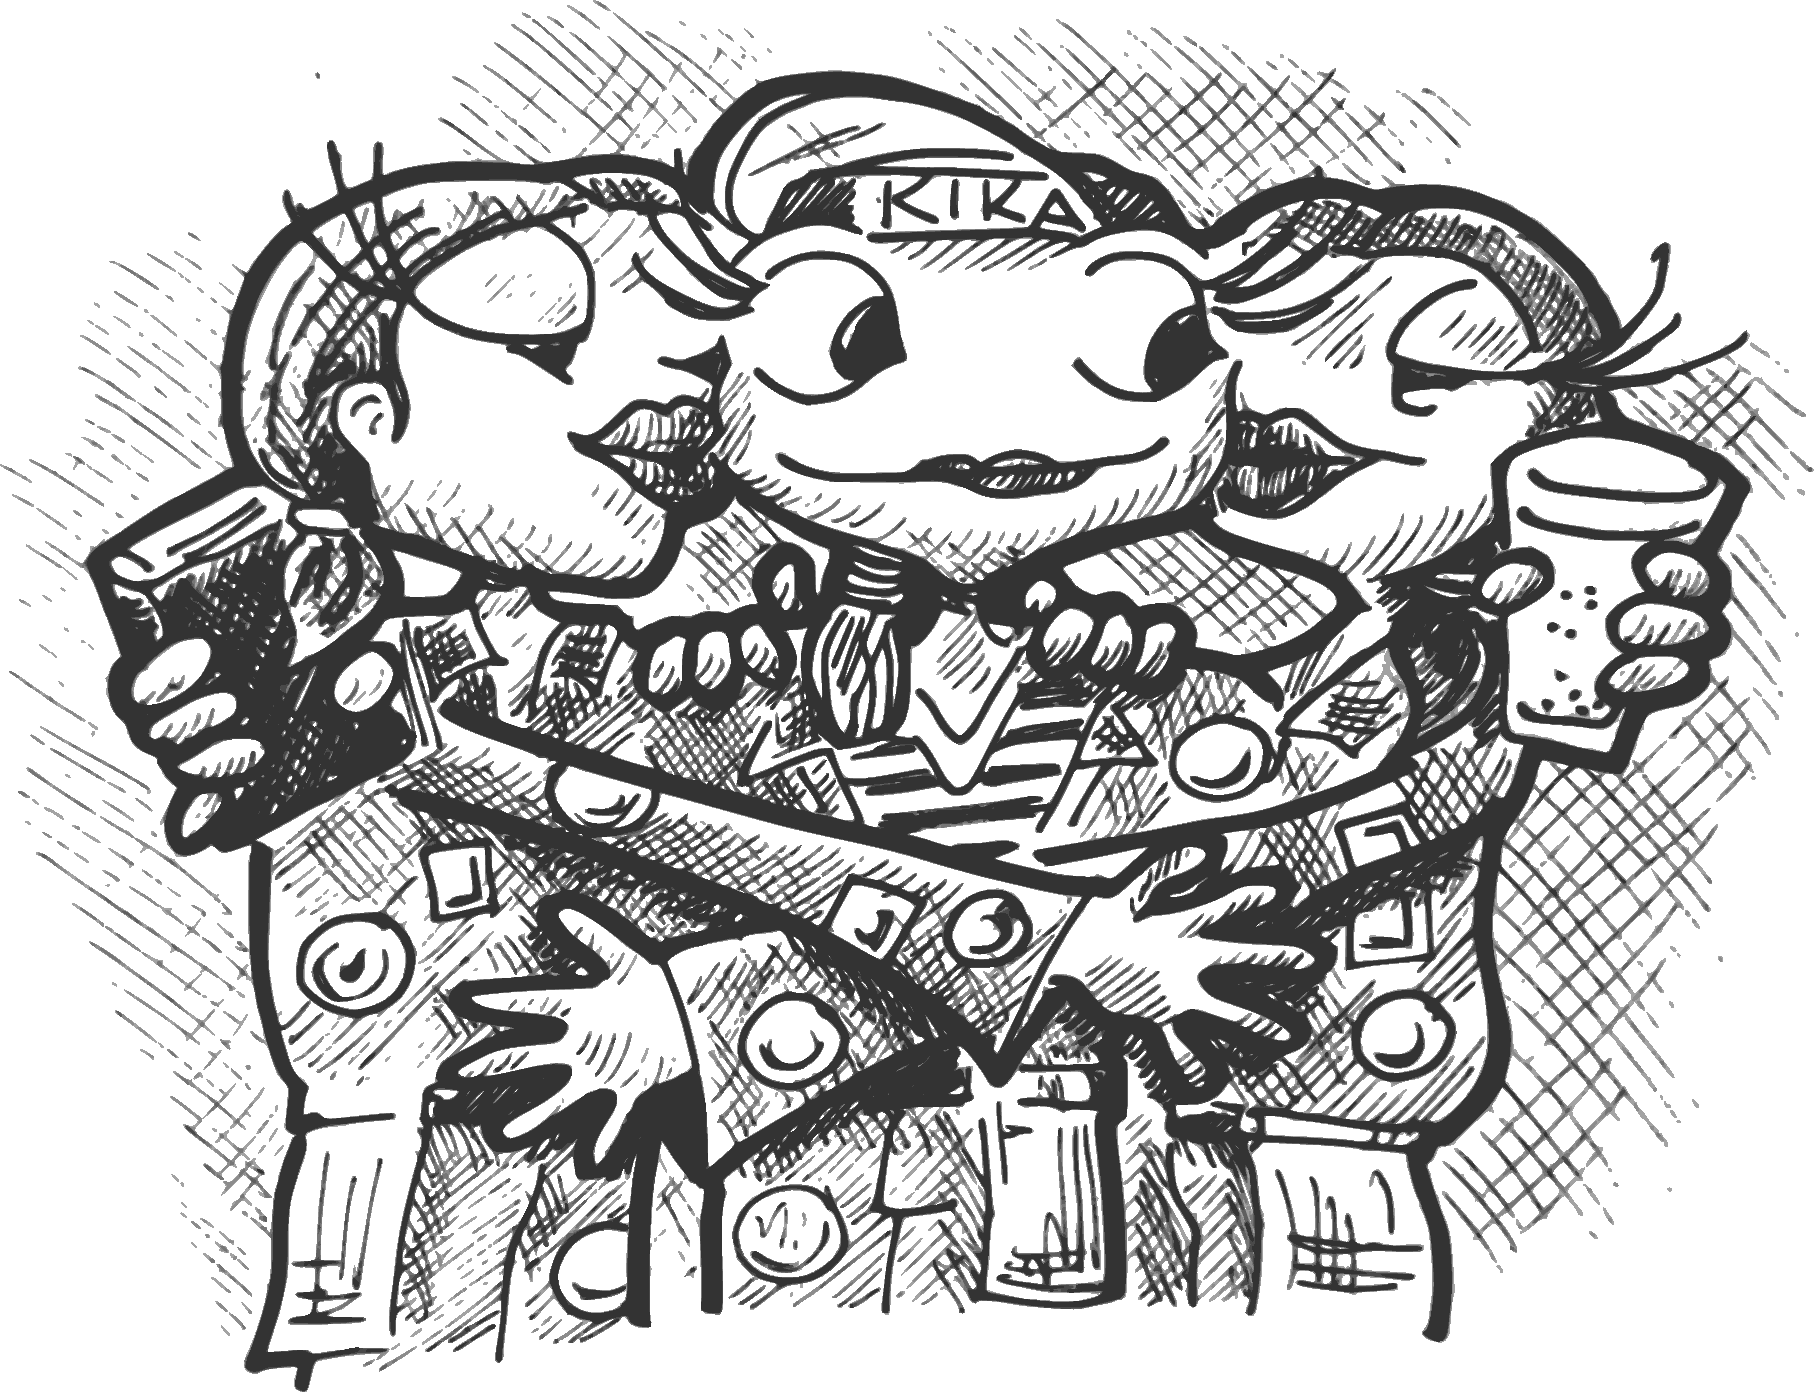
\includegraphics[keepaspectratio,width=\textwidth]{elements/kika.pdf}
\vspace{10pt}\\ Som många andra flyttade jag ifrån min egen familj och
kom ensam till den nya världen på Universitetet.\\\\Denna sida tillägnas
till familjen jag fick första dagen på Pollax - DV familjen.\\\\Tack till
alla ni som är min familj - ni har alltid en plats i mitt
hjärta.\\\\/Erika ``Kika'' Wahlberg (fd Westermark),
DV99\\{\footnotesize\textit{PS blurGel är bäst! DS}} \vfill \null
\newpage
\fvisa{WRITE IN C}{When I find my code in tons of trouble}
{\footnotesize\textit{Melodi: Let it be}}\par
\vspace{10pt}
When I find my code in tons of trouble,\\
friends and colleagues come to me,\\
speaking words of wisdom:\\
``Write in C.''\par
\vspace{10pt}
As the deadline fast approaches,\\
and bugs are all that I can see,\\
somewhere, someone whispers:\\
``Write in C.''\par
\vspace{10pt}
Write in C, write in C,\\
write in C, oh, write in C.\\
LOGO's dead and buried,\\
write in C.\par
\vspace{10pt}
I used to write a lot of FORTRAN,\\
for science it worked flawlessly.\\
try using it for graphics!\\
Write in C.\par
\vspace{10pt}
If you've just spent nearly 30 hours\\
debugging some assembly,\\
soon you will be glad to\\
write in C.\par
\newpage
Write in C, write in C,\\
write in C, yeah, write in C.\\
Only wimps use BASIC.\\
write in C.\par
\vspace{10pt}
Write in C, write in C \\
write in C, oh, write in C.\\
Pascal won't quite cut it.\\
write in C.\par
\vspace{10pt}
Write in C, write in C,\\
write in C, yeah, write in C.\\
Don't even mention COBOL.\\
Write in C.\par
\vspace{10pt}
{\footnotesize\textit{Text: Kriston J. Rehberg}}

\newpage
\fvisa{OM EMACS}{Emacs är en stor koloss}
{\footnotesize\textit{Melodi: Rullan går}}\\
\\
Emacs är en stor koloss.\\
Tugga på, tugga på.\\
Verkar aldrig komma loss.\\
Tugga på, tugga på.\\
För att flytta på ett tecken\\
går två meg i garbage-säcken.\\
Ner i skärmens undre ran’\\
står: garbage collecting, done!\\
\\
Väntar på’n till min pension.\\
Tugga på, tugga på.\\
Emacs gör en Sparcstation\\
Tugga på, tugga på.\\
snabb som en ABC-80.\\
Högprestanda blir så smått i\\
Emacs, den ser säkert till\\
ingen dödtid blir förspilld!\\
\\
Emacs skriven är i Lisp.\\
Tugga på, tugga på.\\
Inget rimmar alls på Lisp.\\
Tugga på, tugga på.\\
Om du in i kärnan trevar\\
finn en gnu som motorn vevar.\\
Den drar Emacs runt för hand!\\
Klart att det går trögt ibland!\\
\\
{\footnotesize\textit{Text: Ingemar Ragnemalm \oldstylenums{1992}}}

\newpage
\fvisa{DET SKA VA' HEMBRÄNT}{Jag har festat mycket, det har inte varit lätt}
{\footnotesize\textit{Melodi: Husvagn}}\par
\vspace{10pt}
Jag har festat mycket, det har inte varit lätt.\\
Blanda vin och whisky, det kan inte vara rätt.\\
Jag har festat på de allra konstigaste sätt,\\
men äntligen jag funnit hur man ska partajja rätt:\par
\vspace{10pt}
Det ska va hembränt, och supa till i några dar.\\
Det ska va hembränt, drick upp det sista ni har kvar.\\
Det ska va hembränt, och svina runt i overall.\\
Det ska va hembränt, drick nu vad ni tål!\par
\vspace{10pt}
I flera år så var vi lite fina där i kanten.\\
Vi smuttade på vinerna men spara aldrig panten.\\
Men sen vi lärde känna våran vackra overall,\\
så super vi nu landet runt på hemgjord alkohol.\par
\vspace{10pt}
Det ska va hembränt ...\par
\vspace{10pt}
Fem små groggar först för att komma igång med festen.\\
Fem små groggar till för att supa ikapp resten.\\
Fem små groggar sen för att kalla det en kväll.\\
Fem små groggar till så sitter vi i fyllecell.\par
\vspace{10pt}
Det ska va hembränt ...\par
\vspace{10pt}
{\footnotesize\textit{Text: Jesper Wilhelmsson, d97}}

\newpage
\fvisa{KOMMANDOTOLKEN}{Far, jag kan inte få upp min kommandotolk}
{\footnotesize\textit{Melodi: Far, jag kan inte få upp min kokosnöt}}\\
\\
Far, jag kan inte få upp min kommandotolk.\\
Alla sätt jag prövat har vart fel;\\
jag har tryckt på knappar, klickat på varje flik,\\
och jag har sagt, “kommandotolk, tack!”,\\
men skärmen är sig lik.\\
\\
Far, jag kan inte få upp min kommandotolk,\\
inte ens med länk till satellit.\\
På varje antenn, har jag satt kopplingssladdar, men,\\
av kommandotolken min syns inte ett skit!\\
\\
Av kommandotolken min syns inte ett ski-i-it!\\
Jag ser bara Emacs, Xfig och Mosaic.\\
Säg, minns du prompten, far?\\
Glöm bort den, är du rar.\\
för av kommandotolken min syns inte ett skit!\\
\\
Far, jag kan inte få upp min kommandotolk,\\
inte ens med nitroglycerin.\\
När jag hade laddat, mycket omsorgsfullt och väl,\\
bortåt jag sprang, sen sa’ det PANG,\\
och Polacksbacken brann ner...\\
\\
Far, jag kan inte få upp min kommandotolk,\\
för jag har ingen hand med dynamit.\\
Av vårt stolta hus, det återstår bara grus,\\
och av kommandotolken min syns inte ett skit!\\
\\
Av kommandotolken min syns inte ett ski-i-it!\\
Allt det andra har blitt lika indefinit (så att säga).\\
Internet står still, vad ska jag ta mig till?\\
Av kommandotolken min syns inte ett skit,\\
ett skit,\\
ett skit,\\
ett skit,\\
Av kommandotolken min syns inte ett ski-i-it!\\
\\
{\footnotesize\textit{Text: Johan Runeson, Nollespexet DVP Uppsala,
    \oldstylenums{1996}\\ \\ (Personligen tycker jag att det ska vara
    ’Fan, jag kan inte...’ /red. anm.)}}

\vspace{15pt}
\visa{MORS LILLA DATOR}
{\footnotesize\textit{Melodi: Mors lilla Olle}}\par
\vspace{10pt}
Mors lilla dator åt skogen gick,\\
mitt i programmet så sade det klick\\
svart bidde skärmen och minnet försvann,\\
den informationen kan ingen få fram.\par
\vspace{10pt}
Brummeli-brum vad brummar där?\\
Det sprakar och gnistrar, ett jordfel det är!\\
Blixtarna blå ifrån burken det slå,\\
synd att jag nu här ensammen stå.\par
\vspace{10pt}
Hyscheli-hysch vad prasslar här?\\
Fram väller pappret ur printern där!\\
Den har fått nippran av tecken så små,\\
jag tror att jag snart hemåt skall gå.

\newpage
\fvisa{ANOTHER GLITCH IN THE CALL}{We don't need no indirection}
{\footnotesize\textit{(sung to the tune of a not so recent Pink Floyd song)}}\par
\vspace{10pt}
We don't need no indirection\\
We don't need no flow control\\
No data typing or declarations\\
Hey! Did you leave the lists alone?\par
\vspace{10pt}
All in all, it's just a pure-LISP\\
function call\par
\vspace{10pt}
We don't need no side effect-ing\\
We don't need no scope control\\
No global variables for execution\\
Hey! Did you leave those args alone?\par
\vspace{10pt}
All in all, it's just a pure-LISP\\
function call\par
\vspace{10pt}
We don't need no allocation\\
We don't need no special nodes\\
No dark bit-flipping in the functions\\
Hey! Did you leave the bits alone?\par
\vspace{10pt}
All in all, it's just a pure-LISP\\
function call
\newpage
We don't need no compilation\\
We don't need no load control\\
No link edit for external bindings\\
Hey! Did you leave that source alone?\par
\vspace{10pt}
All in all, it's just a pure-LISP\\
function call\par
\vspace{10pt}
{\footnotesize\textit{Text: DVLs tidning \#11subscript:8}}

\vspace{15pt}
\fvisa{TUPPENS KLAGOVISA}{Tuppens väckarklocka ringer sex varje morgon}
{\footnotesize\textit{Melodi: Hoppsan vilken dag}}\\
\\
Tuppens väckarklocka ringer sex varje morgon\\
då måste han gå upp till ännu en jävlig dag.\\
Han sätter sig på Teknikum och får genast ångest\\
rysningar i kroppen alla världens obehag.\\
\\
Ännu en föreläsning om fysik och sånt\\
men han tänker på en svettig datasal.\\
Tänk att sitta vid en dator i 1411\\
men miniräknarn är hans enda val.\\
\\
Tuppens verklighet det är ett liv utan glädje\\
gula overaller är ju inget man vill ha.\\
Jag borde ändå gjort som min gamla mamma sa,\\
en DVP:are é va man borde va\\
\revrpt en DVP:are é va man borde va\rpt

\newpage
\fvisa{HALLANDS-SHOT}{Ingen vet det jag vet en hemlighet}
{\footnotesize\textit{Melodi: Margareta}}\par
\vspace{10pt}
Ingen vet det jag vet en hemlighet\\
vad det var i glaset mitt som jag svept\\
kan inte hjälpa att jag känner det så här\par
\vspace{10pt}
Och den kick som jag fick gav mig allt\\
världen börjar snurra runt vad jätteballt\\
tänk att allting känns så härligt när\par
\vspace{10pt}
man dricker Rhoca-Gil ska du veta \\
då blir alla öppningar täta\\
står här bak' en dörr\\
knip' som aldrig förr\\
och kan inte pissa\par
\vspace{10pt}
pulsarna de bränner så heta\\
dricker du som jag ska du veta\\
suparna du tar\\
har du evigt kvar - inom dig\par
\vspace{10pt}
Så jag går ut igen till nästa bar\\
ännu en Hallands-shot jag genast tar\\
tänk att allting känns så härligt när\par
\vspace{10pt}
man dricker Rhoca-Gil ska du veta \\
då blir alla öppningar täta\\
står här bak' en dörr\\
knip' som aldrig förr\\
och kan inte pissa

pulsarna de bränner så heta\\
dricker du som jag ska du veta\\
suparna du tar \\
har du evigt kvar - inom dig\par
\vspace{10pt}
{\footnotesize\textit{Text: Anders Ramsell, Johan Runeson, Henrik Eriksson}}

\vspace{15pt}
\visa{DET VAR FEST NER I FOORUM}
{\footnotesize\textit{Melodi: Det var dans bort i vägen}}\par
\vspace{10pt}
Det var fest ner i FooRum på tisdagsnatten.\\
Upp i trappan gick låten av sången och skratten.\\
Det var tjo! Det var tjim! Det var hej!\\
Där satt dataloger och skåla och söp\\
och skråla och skräna tills hemåt de kröp\\
för dudeli dudeli dej. HEJ!\par
\vspace{10pt}
Där var Starka å Åhus å Renat å Bäsk,\\
där var Herrgårds och Pors som ej luktar av mäsk\\
där var OP och lite Mai Tai.\\
Där var Årsta och Vinbärs och liknande klägg,\\
där var Punsch och likör utav lingon och ägg\\
för dudeli dudeli dej. SKÅL!\par
\vspace{10pt}
{\footnotesize\textit{Text: Andreas Gref, dvl90 Uppsala}}

\newpage
\fvisa{DATAVETARNAS PARADMARCH}{Ja, här kommer datavetare}
{\footnotesize\textit{Melodi: Fritjof Anderssons paradmarch}}\par
\vspace{10pt}
Ja, här kommer datavetare\\
med märken på vår dräkt.\\
Vi knappar kod, \\
vi hackar LISP\\
och surfar runt på nätet.\par
\vspace{10pt}
Vi lämnar pöbeln stående\\
och gapande förskräckt.\\
Det vi inte kan, \\
det kan ingen ann -\\
nu går vi upp i labbet.\par
\vspace{10pt}
Och när vi loggat ut,\\
ja då går vi på någon fest\\
och tar oss några bira,\\
för det gillar vi ju bäst!\par
\vspace{10pt}
För där är där vi inte är\\
och här är där vi är!\\
Vi knappar kod,\\
vi hackar LISP\\
och festar runt Sverige.\par
\vspace{10pt}
{\footnotesize\textit{Text: Selander, C93 \& Daniel ``Holm''
    Holmgren, C96.\\ Skrevs i baksätet på en Toyota Camry, på väg
    till linjekonferensen -97 i Uppsala. Omdöpt av Jubileumsgruppen
    inför 30 år jubiléet i Uppsala}}

\newpage
\fvisa{OH, LJUVA ÖL}{Jag har nu fått en och annan öl}
{\footnotesize\textit{Melodi: Kung Louis sång}}\\
\\
Jag har nu fått en och annan öl,\\
som jag genast druckit har.\\
Ja, jag har druckit mycket jag.\\
Jag ingen droppe spar.\\
För nu vill jag bara festa,\\
tills jag far ikull.\\
Jag vill ej längre nykter va.\\
Jag vill bara vara full.\\
\\
Oh, ljuva öl, vad jag är glad åt öl.\\
För jag vill dricka den, och en till, öl.\\
Det vill jag nu, ett djur som jag,\\
det lär sig bra bli en fyllehund.\\
\\
Försök inte hindra mig gosse,\\
för nu så är det fest.\\
Och då man drycker dricka ska,\\
som gjorda är på jäst.\\
Så ge mig nu inget annat,\\
att hälla i mitt glas.\\
för nu så ska jag dricka ur,\\
och bli full som ett as.

\newpage
\fvisa{IT IS FREE}{When I find myself in front of Windows}
{\footnotesize\textit{Melodi: Let It Be}}\par
\vspace{10pt}
When I find myself in front of Windows,\\
Father Torvalds comes to me,\\
Speaking words of Linux, ``It is free!''.\\
And when hackers crack my system\\
through some strange NT obscurity,\\
he gives me the source-code, ``It is free!''.\par
\vspace{10pt}
It is free, it is free, it is free, it is free.\\
Linux is the answer, and it's free.\par
\vspace{10pt}
When the broken system crashes\\
and blue screens of death I see.\\
There is one true rescue, and it's free.\\
For though there may be doubts first\\
it will sure bring life to your PC\\
`Cause Linux is the answer, and it's free.\par
\vspace{10pt}
It is free, it is free, it is free, it is free,\\
You even get the source-code, it is free.\par
\vspace{10pt}
In the darkest night, when hacking,\\
Xfree stares right back at me,\\
Now I've installed Linux, I feel free.\\
No longer mad with my computer,\\
No more does it crash on me\\
Now I've installed Linux, it is free.
\newpage
It is free, it is free, it is free, it is free,\\
Open-sourced true power, it is free.\par
\vspace{10pt}
{\footnotesize\textit{Text: David Weinehall}}

\chapterpage{Snapsvisor}{Snapsvisor}
\section{SUPARNAS ORDNING}\index{SUPARNAS ORDNING}
\vspace{10pt}
\begin{enumerate}[leftmargin=0.65cm,topsep=0pt,itemsep=0pt,partopsep=0pt,parsep=3pt]
\item Helan
\item Halvan
\item Tersen.
\item Kvarten
\item Kvinten
\item Sexten
\item Septen
\item Rivan
\item Rafflan.
\item Rännan
\item Smuttan
\item Smuttans unge
\item Femton droppar
\item Lilla Manasse
\item Lilla Manasses Broder
\item Klämtaren
\item Kreaturens återuppståndelse
\item Den bleka dödens dryck
\item Krokofanternas intåg
\item Ett evigt liv
\end{enumerate}
\newpage
\section{ANVISNINGAR FÖR SNAPSENS TAGANDE}\index{ANVISNINGAR FÖR SNAPSENS TAGANDE}
\vspace{10pt}
\begin{itemize}[leftmargin=0cm,topsep=0pt,itemsep=2pt,partopsep=0pt,parsep=3pt,label={}]
\item Snapsen tages till fisk.
\item All mat är fisk, förutom ölsupa och pannkaka.
\item Den som äter ölsupa eller pannkaka, sup på grannens fisk.
\item Skulle grannen förtära ölsupa eller pannkaka, må även dessa rätter betraktas som fisk.
\item Desserten ätes med gaffel, så länge det går, därefter med sked.
\item Man må icke dricka ur sköljkopparna.
\item Ty den goda törsten bör släckas med ädlare fludium än tvättvatten.
\item Vatten betraktas aldrig som fisk.
\end{itemize}
\newpage
\visa{2*7 och en halv}
{\footnotesize\textit{Melodi: Lambert Walk}}\\
\\
2 * 7 1/2 = 12\\
Än kan vi skilja på tak och golv!\\
2 * 5 = 7\\
Hur i helvete räknar du?\\

\vspace{15pt}
\fvisa{ATT TA SIG}{Att ta sig en riktig hela}
{\footnotesize\textit{Melodi: Flickan hon går i dansen}}\\
\\
Att ta sig en riktig hela\\
det är ju ett bruk.\\
På den ska man inte dela\\
då kan man bli sjuk.\\
Hormoner och kalk och C-vitamin\\
är ingenting mot kallt brännevin.

\newpage
\fvisa{Alkotest}{Båd' sommar och vinter när snapsen}
{\footnotesize\textit{Melodi: Titta det snöar}}
\begin{center}
  Båd' sommar och vinter när snapsen\\
  den slinter i pojkar och stinter\\
  går bra - går bra. Och nu vi\\
  ej töva vår nykterhet pröva\\
  och sjunga och öva - går\\
  bra - går bra! Ett visst\\
  kvistfritt kvastskaft\\
  och kaffekask dags\\
  strax sex laxar\\
  i laxask går\\
  bra - går\\
  bra! Den\\
  provet\\
  kan\\
  klara\\
  han\\
  kan\\
  utan fara\\
  ta snapsen och svara\\
  MÅR BRA - MÅR BRA!
\end{center}

\chapterpage{Ölvisor}{Ölvisor}

\chapterpage{Vinvisor}{Vinvisor}
\fvisa{GLÖGGVISA}{Vi ser det snöar}
{\footnotesize\textit{Melodi: Vi ser det snöar}}\par
\vspace{10pt}
Vi ser det snöar,\\
vi ser det snöar,\\
och glöggen vi tar.\\
Vi ser det snöar,\\
vi ser det snöar,\\
varmt i magen hurra!\\
Nu tar vi russinen fram\\
att krydda den med.\\
Sedan magen den får,\\
Och hej vad den mår.

\vspace{15pt}
\fvisa{GLÖGGVISAN}{Ack, glöggen den står på bordet}
{\footnotesize\textit{Melodi: Flickan hon går i ringen}}\\
\\
Ack, glöggen den står på bordet\\
och ångar sig varm.\\
Vi häller den ner i halsen \\
och värmer vår tarm.\\
En här, en där, utan minsta besvär,\\
den drycken är vår strupe så innerligt kär!

\newpage
\visa{SUDDA SUDDA}
{\footnotesize\textit{Melodi: Sudda sudda}}\\
\\
Sudda sudda sudda sudda bort din sura min\\
Med fyra jättestora bamseklunkar ädelt vin.\\
Munnen den ska sjunga och va' glad'.\\
För att den ska bli som den ska va'.\\
Vad häller du då bak det dolda flinet?\\
Vinet, som suddar suddar bort din sura min.

\vspace{15pt}
\fvisa{UNDULATEN}{Jag är en liten undulat}
{\footnotesize\textit{Melodi: Med en enkel tulpan}}\\
\\
Jag är en liten undulat\\
som får så dåligt med mat\\
för dom jag bor hos\\
ja dom jag bor hos\\
dom är så snåla.\\
Jag får ju fisk varenda dag\\
men det vill jag inte ha\\
jag vill ha rödvin\\
jag vill ha rödvin och gorgonzola

\newpage
\fvisa{SOLSKEN I BLICK}{Sjungom så glada till glasens klang}\\
{\footnotesize\textit{Melodi: Mors lilla Olle}}\\
\\
Sjungom så glada till glasens klang\\
vinet det har både heder och rang\\
Alla så får vi på ett ögonblick\\
rosor på kinden och solsken i blick.\\
\\
Gudarnas gåva. O, vilken fröjd.\\
Dofterna stiga mot himlens höjd.\\
Noak planterade vin och han fick\\
rosor på kinden och solsken i blick.\\
\\
Trivsamt och festligt det ska det va'\\
vinet gör människan vänlig och glad\\
vinet ger färg åt den blekaste prick\\
rosor på kinden och solsken i blick.\\
\\
Bröder och systrar nu höj ditt glas.\\
Vinet förljuvar vårt glada kalas.\\
Drick ur ditt glas och du får på ett kick\\
rosor på kinden och solsken i blick.\\
\\
Låtom oss glädjas och kasta loss.\\
Festföremålet skall säga om oss:\\
Gästerna hade, då hemåt de gick\\
rosor på kinden och solsken i blick.

\newpage
\fvisa{FRANSK VINVISA}{Feta fransyskor som svettas om fötterna}
{\footnotesize\textit{Melodi: Schuberts militärmarsch (Tomtarnas vaktparad.)}}\par
\vspace{10pt}
Feta fransyskor som svettas om fötterna,\\
de trampa druvor som sedan ska jäsa till vin.\\
Transpirationen viktig é,\\
ty den ger fin bouquet.\\
Vårtor och svampar följer mé\\
men vad gör väl dé?\par
\vspace{10pt}
För vi vill ha vin, vill ha vin, vill ha mera vin\\
även om följderna bli att vi må lida pin\par
\begin{tabular}{@{}m{0.05\linewidth}p{0.7\linewidth}@{}}
  \scalebox{1.5}{\Female} & Flaskan och glaset gått i sin\\
  \scalebox{1.5}{\Male} & Hit med vin, mera vin\\
  \scalebox{1.5}{\Female} & Tror ni att vi är fyllesvin\\
\end{tabular}\par
(\textit{skrik}) Ja, fast större!\par
\vspace{10pt}
{\footnotesize\textit{Text: Helène Derand\\Sångarstriden 1985 av
    K-LTH}}

\vspace{15pt}
\fvisa{VINETS LOV}{Läppar friska, pocka viska. Skål på Er.}
{\footnotesize\textit{Melodi: Punschen kommer}}\\
\\
Läppar friska, pocka viska. Skål på Er.\\
Strupar klara, sjunga svara, skål på Er.\\
Skål för glada minnen, skål för evig vår,\\
Inga sorger finnas mer, när vin vi får.

\chapterpage{Avecvisor}{Avecvisor}
\fvisa{PUNSCHEN DET BÄSTA ÄR}{Glasen nu fyllas}
{\footnotesize\textit{Melodi: Vårvindar friska}}\par
\vspace{10pt}
Glasen nu fyllas. Punschen bör hyllas\\
såsom den är - ett livselexir!\\
Om kraften sinar, kroppen förtvinar,\\
med detta guld så finner man liv.\\
Ja, denna dryck den är vår passion.\\
En äkta vitamininjektion.\\
Man får förmoda; bland livets goda\\
punschen det bästa är!\par
\vspace{10pt}
{\footnotesize\textit{Ur spexet Unionsupplösningen från 1988 Norrlands Nation i Uppsala}}

\vspace{15pt}
\fvisa{LILLA PUNSCHVISAN}{Det var en gång jag tänkte att punschen övergiva}
{\footnotesize\textit{Melodi: Te deum Laudamus}}\par
\vspace{10pt}
Det var en gång jag tänkte att punschen övergiva,\\
men det får inte ske, så länge jag får leva.\\
Och när jag en gång dör, så står det på min grav:\par
\vspace{10pt}
``Här vilar en som svenska punschen älskat har''\\
Jag gillar, jag gillar punschen.\\
Jag gillar den som punschen skapat har.\\
Jag gillar, jag gillar punschen.\\
Jag gillar punschen och dess far.\par
\vspace{10pt}
{\footnotesize\textit{Ur Skogshögskolans sångbok, 1906}}

\newpage
\fvisa{PUNSCH ELLER KONJAK}{Ska det inte bli nån punsch ikväll?}
{\footnotesize\texit{Melodi: Play a Simple Melody}}\\
\\
Ska det inte bli nån punsch ikväll?\\
Jag har väntat middan lång.\\
Punschen, kom och gör mig god och snäll.\\
Punschen kommer du nån gång?\\
\\
Punsch ger själen frid, får hjärtat slå.\\
Bra för ande och för kropp.\\
Hit med Cederlunds och Grönstedts Blå\\
och låt Flaggpunsch gå i topp.\\
\\
Punsch OK, men ingenting för mig.\\
Punschen saknar all bouqet.\\
Är det det som du har tänkt att ge\\
har jag en bättre idé.\\
\\
Ge mig konjak för det gör mig säll.\\
Courvoisier eller Martell.\\
Remy Martin det kan väl gå.\\
Annars får det bli Renault.\\
\\
{\footnotesize\texit{Vers 1 och 2 sjungs av de punsch drickande, 3 och 4 av de konjaks drickande.}}

\newpage
\fvisa{ÄNGLAPUNSCHEN}{Kalla den gudagåva eller himlanektar, vad du vill}
{\footnotesize\textit{Melodi: Änglamark}}\\
\\
Kalla den gudagåva eller himlanektar, vad du vill\\
punschen den gyllne, de gamle oss skänkte.\\
Vet att så länge som punschen nånsin funnits till\\
glädjen den höjde och sorgerna dränkte.\\
\\
Blunda och dröm om en blommande sommarnatt\\
svala bersåer där punschen står immig.\\
Eller en höstdag när Nordan har lekt tafatt\\
varm punsch som ångar och ärtsoppa simmig.\\
\\
Punschen den älskas ju av alla och en var.\\
Låt festen börja - låt punschen flöda!\\
Skål alla vänner som har nå’t i glasen kvar,\\
hedra nu minnet av gamle Kung Oscars da'r!\\
\\
Kalla den gudagåva eller himlanektar, vad du vill\\
punschen den gyllne, som får oss att drömma.\\
Fukta din strupe, låt inte flaskan stå still,\\
skåla för punschen och glasen vi tömma.

\newpage
\fvisa{TVEKAN INFÖR PUNSCHEN}{Jag borde nog inte dricka mer}
{\footnotesize\textit{Melodi: Rosa på bal }}\par
\vspace{10pt}
Jag borde nog inte dricka mer\\
varken öl eller vin eller brännevin.\\
En kaffetår blott, men såvitt jag ser\\
står det punsch brevi'n.\par
\vspace{10pt}
Tänk vilken underbar färg och odör \\
 - nej, det blir bara man bråkar och stör.\\
Men för att inte min kväll skall bli trist,\\
krävs både slughet och list!\par
\vspace{10pt}
Så jag tror nog att jag tar en\\
punsch, kanske två, kanske tre!\\
Sen blir det groggar i baren,\\
jag klarar säkert av det!\par
\vspace{10pt}
Trots att jag egentligen är rätt knall,\\
piggar nog punsch upp mig i alla fall.\\
Jag kvicknar till med en punsch i min bål.\\
Nu har jag bestämt mig, SKÅL!

\newpage
\visa{VI VILL HA PUNSCH}
{\footnotesize\textit{Melodi: tema ur familjen Adams}}\par
\vspace{10pt}
Vi vill ha punsch, (knäpp, knäpp)\\
vi vill ha punsch, (knäpp, knäpp)\\
vi vill ha punsch, vi vill ha punsch,\\
vi vill ha punsch. (knäpp, knäpp)\par
\vspace{10pt}
När man vill festen liva,\\
upp är det bra att kliva,\\
omkring på bordets skiva\\
och klafsa runt i punsch.\par
\vspace{10pt}
Klafsa i punsch, (slurp, slurp)\\
klafsa i punsch, (slurp, slurp)\\
klafsa i punsch, klafsa i punsch,\\
klafsa i punsch. (slurp, slurp)

\vspace{15pt}
\fvisa{FESTU:s PUNSCHVISA}{Punschen, punschen rinner nerför strupen}
{\footnotesize\textit{Melodi: Tomtarnas julnatt}}\par
\vspace{10pt}
Punschen, punschen rinner nerför strupen\\
ner för strupen.\\
Blandas, konfronteras där med supen\\
där med supen\\
Gula droppar stärker våra kroppar\\
punsch, punsch, punsch

\newpage
\fvisa{PUNSCHVISA}{Nu med en ny och stadig krök}
{\footnotesize\textit{Melodi: Med en enkel tulipan}}\\
\\
Nu med en ny och stadig krök\\
med armen gör vi försök\\
att lyfta koppen, att lyfta koppen\\
som står och väntar.\\
\\
Håll blicken fäst vid koppens rand \\
och darra inte på hand.\\
Nu allesammans, nu allesammans\\
på munnen gläntar.\\
\\
En liten punschtår så här placerad\\
i ena handen sig bättre gör\\
än tio liter uppå Systemet\\
och inga pengar att köpa för.\\
\\
Spill inga droppar på ditt bord\\
och spill ej mer några ord.\\
Nu tar vi punschen, nu tar vi punschen\\
som står och väntar

\newpage
\visa{PUNSCHEN KOMMER (KALL)}
{\footnotesize\textit{Melodi: Vals ur Glada Änkan}}\par
\vspace{10pt}
Punschen kommer, punschen kommer\\
ljuv och sval.\\
Glasen imma, röster stimma\\
i vår sal.\\
Skål för glada minnen!\\
Skål för varje vår!\\
Inga sorger finnas mer,\\
när punch vi får.

\vspace{15pt}
\visa{PUNSCHEN KOMMER (VARM)}
{\footnotesize\textit{Melodi: Vals ur Glada Änkan}}\par
\vspace{10pt}
Punschen kommer, punschen kommer\\
god och varm.\\
Vettet svinner, droppen rinner\\
ner i tarm.\\
Skål för alla minnen\\
vi snart mer ej ha,\\
då ett par glas ljuvlig punsch\\
vi hunnit ta.

\newpage
\visa{GOLDEN DROPS}
{\footnotesize\textit{Melodi: Tomtarnas julnatt}}\\
\\
Golden drops are nice, I have reflected,\\
have reflected.\\
But their strength is not to be neglected,\\
be neglected.\\
Both your head and heart will be affected,\\
punsch, punsch, punsch!

\chapterpage{Gasquevisor}{Gasquevisor}
\visa{VÄLKOMMEN HIT}
{\footnotesize\textit{Melodi: Jänta å ja}}\par
\vspace{10pt}
Välkommen hit, tag er en bit\\
njut utav maten vi tagit hit.\\
Skoj ska vi ha, dansa vi ska\\
trivas så där förtroligt.\\
Humöret på alla toppen ska nå\\
skratta och sjunga det ska vi få.\\
Nöjda med festen hemåt vi gå.\\
I kväll ska vi ha det roligt.

\vspace{15pt}
\fvisa{TILL DRYCKERNAS ÄRA}{Vin är gott men öl är ljuvligt}
{\footnotesize\textit{Melodi: Här är gudagott att vara}}\par
\vspace{10pt}
Vin är gott men öl är ljuvligt\\
tänk vad snapsen värmer gott.\\
Kvällen våt och morgonen gruvlig.\\
Tänk att livet ändå är kort.\\
Punschen guldgul, konjak dito.\\
Vatten smakar inte gott.\\
Lär din läxa, drick ej lite.\\
Drick ur varje glas du fått.\par
\vspace{10pt}
{\footnotesize\textit{Text: Ove Andersson\\ \\ Ur spexet Jämmerdal,
    1994, Norrlands Nation i Uppsala}}

\newpage
\fvisa{VÅR UNGDOMS FAGRASTE VÅR}{Det var i vår ungdoms fagraste vår}
\vspace{10pt}
Det var i vår ungdoms fagraste vår,\\
vi drack varandra till,\\
och vi sade gutår!\\
Alla så dricka vi N.N till.\par
\vspace{10pt}
{\textbf N.N han säger inte nej därtill.}\par
\vspace{10pt}
För det var i vår ungdoms fagraste vår,\\
vi drack varandra till,\\
och vi sade gutår! 

\vspace{15pt}
\fvisa{SIFFERVISAN}{1 2 sjuttiofem 6 7}
{\footnotesize\textit{Melodi: Ritsch ratsch...}}\par
\vspace{10pt}
1 2 sjuttiofem 6 7, sjuttiofem 6 7, sjuttiofem 6 7\\
1 2 sjuttiofem 6 7, sjuttiofem 6 73\\
107 103 102\\
107 6 19 27\\
17 18 16 15\\
13 19 14 17\\
19 16 15 11\\
8 42

\newpage
\visa{JAG HAR ALDRIG VART PÅ SNUSEN}
{\footnotesize\textit{Melodi: O hur saligt att få vandra}}\par
\vspace{10pt}
Jag har aldrig vart på snusen,\\
aldrig rökat en cigarr, halleluja!\\
Mina dygder äro tusen,\\
inga syndiga laster jag har.\\
Jag har aldrig sett nåt naket,\\
inte ens ett litet nyfött barn!\\
Mina blickar går mot taket,\\
därmed undgår jag frestarens garn, halleluja!\par
\vspace{10pt}
Halleluja...\par
\vspace{10pt}
Bacchus spelar på gitarren,\\
satan spelar på sitt handklaver!\\
Alla djävlar dansar tango,\\
säg vad kan man väl önska sig mer?\\
Jo, att alla bäckar vore brännvin,\\
Fyrisån var full av bayerskt öl.\\
Konjak i varenda rännsten\\
och punsch i varendaste pöl, mera öl!\par
\vspace{10pt}
Mera öl...\par
\vspace{10pt}

\newpage
\fvisa{KAMELEN PÅ KANELEN}{Om jag vore ett tvåpuckligt djur}
{\footnotesize\textit{Melodi: Old McDonald}}\par
\vspace{10pt}
Om jag vore ett tvåpuckligt djur\\
Eta-eta-nol\\
Kunde jag super i ur och skur\\
Eta-eta nol\\
Fett, fett, fett, bärverfett\\
Bäverfett gör livet lätt\par
\vspace{10pt}
När man går i Kemikums öken\\
Eta-eta-nol\\
Vill man gärna ta till kröken\\
Eta-eta-nol\\
Fett, fett, fett, ...\par
\vspace{10pt}
När jag spriten lagrat upp\\
Eta-eta-nol\\
Klår jag lättans upp en mupp\\
Eta-eta-nol\\
Fett, fett, fett, ...\par
\vspace{10pt}
Nu när nubben slinker ner\\
Eta-eta-nol\\
Jag redan längar efter mer\\
Eta-eta-nol\\
Fett, fett, fett, ...

\newpage
\visa{DOM SOM ÄR NYKTRA}
{\footnotesize\textit{Melodi: Du är den ende}}\par
\vspace{10pt}
Dom som är nyktra har inte så roligt\\
dom har bara ansvar och inte nåt tjolit-\\
an-lej-faderulla, men vi som är fulla\\
vi har bara kul nästan jämt.\par
\vspace{10pt}
Det sägs att en männ'ska kan va' utan brännvin\\
det stämmer kan hända men se blott den min\\
som pryder en absolutist den är djävligt trist\\
därför sjunger vi så:\par
\vspace{10pt}
Dom som är...

\vspace{15pt}
\fvisa{SÅ LÄNGE}{Så länge rösten är mild}
{\footnotesize\textit{Melodi: Så länge skutan kan gå}}\\
\\
Så länge rösten är mild,\\
så länge ingen är vild,\\
så länge spegeln på väggen ger halvskaplig bild.\\
Så länge alla kan stå,\\
så länge alla kan gå,\\
så länge alla kan tralla så fyller vi på.\\
För vem har sagt att just du kom med storken,\\
för att bli glad av att lukta på korken?\\
Men kring vårt bord här nånstans\\
vi höjer bägaren med glans,\\
och låter vinet gå ner med en yrande dans.

\newpage
\visa{VI SOM ÄR NYKTRA}
{\footnotesize\textit{Melodi: Du är den ende}}\par
\vspace{10pt}
Vi som är nyktra vi har faktiskt roligt.\\
Jo visst har vi ansvar, men minst lika tjolitt-\\
anlej faderulla som ni som är fulla\\
som tror ni har kul nästan jämt.\par
\vspace{10pt}
Men tänk då efter uppå dagar efter\\
de dagar med fester, med smärtsamma rester\\
utav eran hjärna, nog tycker ni gärna:\\
``Att va' nykterist är nå't visst.''\par
\vspace{10pt}
Vi som är nyktra, vi har bara roligt.\\
Imorr'n kan vi återigen ha det tjolitt-\\
anlej faderulla, men ni som var fulla\\
aj, aj, aj, det är väl för trist.

\vspace{15pt}
\visa{TAG NU DJUPA KLUNKAR}
{\footnotesize\textit{Melodi: Lili Marlene}}\par
\vspace{10pt}
Tag nu djupa klunkar,\\
sjung och drick, var glad.\\
Innan gänget lunkar\\
på festprisseparad.\\
Vad gör väl det om våra ben\\
då vingla lätt på gatans sten.\\
När vi beger oss hem.\\
Vi undrar blott till vem.

\newpage
\visa{JAG VAR FULL EN GÅNG}
{\footnotesize\textit{Melodi: Flottarkärlek}}\par
\vspace{10pt}
Jag var full en gång för länge sen,\\
på knäna kröp jag hem.\par
\vspace{10pt}
Varje dike var för mig ett vilohem.\\
I varje skåp, i varje vrå\\
hade jag en liten vän,\\
ifrån renat upp till 96 procent, procent.\par
\vspace{10pt}
Jag var full...\\
Och som sällskap hade jag en elefant.\\
Elefanten spruta vatten,\\
men jag trodde det var vin,\\
sedan dess har alla kallat mig för svin, mera vin.\par
\vspace{10pt}
Jag var full...\\
Och som sällskap hade jag en elefant.\\
Elefanten spruta vatten,\\
men jag trodde det var öl,\\
sedan dess har alla kallat mig för knöl, mera öl.\par
\vspace{10pt}
Jag var full...\\
Och som sällskap hade jag en elefant.\\
Elefanten spruta vatten,\\
men jag trodde det var sprit\\
sedan dess har alla kallat mig för skit, mera sprit

\newpage
\fvisa{LAMBO}{Sätt nu glaset till din mun"!}
\vspace{10pt}
Sätt nu glaset till din mun!\\
Tjofaderitan, lambo!\\
Och drick ur din fylle-, fyllehund!\\
Tjofaderitan, lambo!\\
Se hur dropparna i glaset\\
rinner ner i fylleaset.\\
Lambo hej, lambo hej, \\
tjofaderitan lambo!\\
\\
\textbf{Jag nu glaset druckit har!}\\
Tjofaderitan lambo\\
\textbf{Ej en droppe finnes kvar!}\\
Tjofaderitan lambo.\\
\textbf{Som bevis jag nu vill vända\\
glaset på dess ``rätta'' ända.}\\
Lambo hej, lambo hej\\
tjofaderitan lambo.\\
\\
Ja, han kunde konsten,\\
han var en äkta fylle-, fyllehund.\\
Så låt oss gå till nästa man\\
och se vad han förmår\\
\\
(\textit{En liten variant})\\
\textbf{Som bevis jag nu vill föra\\
glaset till min grannes öra}

\newpage
\fvisa{NIKOLAJEV}{Jag heter Nikolajev}
{\footnotesize\textit{Melodi: Sovjetunionens nationalsång}}\par
\vspace{10pt}
Jag heter Nikolajev\\
och kommer från Sovjet.\\
Jag flyger runt jorden\\
i min rymdraket.\\
Och där ska jag stanna i 84 varv\\
för det har Chrustjev sagt\\
men det tycker jag är larv.\par
\vspace{10pt}
Jag längtar hem, hem till min planet.\\
Till fru och barn därhemma i Sovjet.\\
Men mest utav allt längtar jag till ett rum\\
med ett hjärta på dörren.\\
Jag längtar hem till min planet\\
till fru och barn därhemma i Sovjet\par
\vspace{10pt}
Min kapsel innehåller\\
många instrument.\\
Ja, mycket av sådant\\
som ännu ej är känt.\\
Men lika förbannat, vad du än tror:\\
Jag glömde gå på muggen\\
innan jag for.\par
\vspace{10pt}
Jag längtar hem...
\par
\vspace{10pt}
{\footnotesize\textit{Uppsala teknologernas signarturmelodi, datavetare sitter ner när den sjungs.}}

\newpage
\fvisa{MINNE}{Minne"! Jag har tappat mitt minne}
{\footnotesize\textit{Melodi: Memory ur musikalen Cats}}\\
\\
Minne! Jag har tappat mitt minne\\
är jag svensk eller finne?\\
Kommer inte ihåg\\
\\
Inne! Är jag ute eller inne?\\
Jag har luckor i minne\\
såna där små alkohol.\\
\\
Men besinne, man tätar det med brännvin \\
som man får fastän minnet \\
och helan den går.\\
\\
{\footnotesize\textit{Text: Bosse Österberg}}

\vspace{15pt}
\visa{DET VAR LÄNGE SEN}
{\footnotesize\textit{Melodi: Det var länge sin jag plocka några blommor}}\par
\vspace{10pt}
Det var länge sen jag plocka' några blommor.\\
Det var länge sen jag tog några poäng.\\
Det var länge sen jag handla' på systemet.\\
Det var länge sen jag fick en tjej/kille i säng.\par
\vspace{10pt}
Men å andra sidan bränner jag ju hemma,\\
och klarar kärleken alldeles för mig själv.\\
Det var länge sen jag plocka' några tentor\\
men å andra sidan går de om igen.

\newpage
\fvisa{KALMAREVISAN}{För uti Kalmare stad}
\vspace{10pt}
\textbf{För uti Kalmare stad}\\
ja där finns det ingen kvast\\
förrän lördagen.\\
\textbf{Hej dick}\\
Hej dack\\
\textbf{Jag slog i}\\
och vi drack\\
\textbf{Hej dickom dickom dack}\\
hej dickom dickom dack.\\
För uti Kalmare stad\\
ja där finns det ingen kvast\\
förrän lördagen.\\
\\
\revrpt \textbf{När som bonden kommer hem}\\
kommer bondekvinnan ut\rpt\\
och är stor i sin trut\\
\textbf{Hej dick...}\\
\\
\revrpt \textbf{Var är pengarna du fått?}\\
Jo, dom har jag supit opp!\rpt\\
Uppå Kalmare slott.\\
Hej dick...\\
\\
\revrpt \textbf{Jag skall mäla dig an}\\
för vår kronbefallningsman\rpt\\
Och du skall få skam\\
\textbf{Hej dick...}
\newpage
\revrpt \textbf{Kronbefallningsmannen vår}\\
satt på krogen i går\rpt\\
Och var full som ett får.\\
\textbf{Hej dick...}\\
\\
{\footnotesize\textit{Text: G S Kallstenius}}\\
\\
(\textit{Tre små tillägg})\\
\revrpt \textbf{Va' sa' bonnen ha te' mat?}\\
Sura sillar och potat\rpt\\
det blir sillsallat.\\
\textbf{Hej dick...}\\
\\
\revrpt \textbf{Säg var är din lab-rapport}\\
Jo, den har jag supit bort!\rpt\\
För den var så kort!\\
\textbf{Hej dick...}\\
\\
\revrpt\textbf{Ordföranden vår}\\
var på 100-kör igår.\rpt\\
Dom bar ut han på bår!\\
\textbf{Hej dick...}\\
\\
{\footnotesize\textit{I Linköping är det inget ``Hej dick...''-ande på
    första versen, dock reprisande som följande verser.}}

\newpage
\fvisa{VIKINGEN}{En viking älskar livets vann}
{\footnotesize\textit{Melodi: When Johnny comes marching home}}\par
\vspace{10pt}
En viking älskar livets vann\\
Hurra, hurra!\\
Den hastigt i mitt svalg försvann\\
Hurra, hurra!\\
Till kalv, till oxe, till fisk, till fläsk,\\
när kärringar bara dricker läsk.\\
Ja, då vill alla vikingar ha en bäsk.\par
\vspace{10pt}
När bäsken småningom är slut\\
Tragik, tragik\\
Då bäres varje viking ut\\
som lik, sig lik\\
Och sen, om vi vaknar, vi sjunger en bit,\\
sen korkar vi upp Skånes Aquavit\\
Skål för alla vikingar som kom hit!\par
\vspace{10pt}
{\footnotesize\textit{Sångarstriden 1981 av E-LTH}}\par
\vspace{10pt}
Och datavetaren minsann,\\
vill också ha\\
en bäsk till maten då och då\\
det sitter bra\\
När datavetarens väg är klar\\
han lämnat inte en droppe har\\
skål för alla vikingar som finns kvar\par
\vspace{10pt}
{\footnotesize\textit{Text: Carl Leonardsson, Anders Steinrud, Niclas Stensbäck, Samuel Strand}}

\newpage
\visa{WE ARE SAILING}
%% {\footnotesize\textit{Melodi: Sailing}}\\
%% \\
\vspace{10pt}
We are sailing, we are sailing,\\
through the water, across the sea.\\
We are sailing, lugna waters,\\
to be ute, to be free.
\vspace{12pt}\\
\begin{tabular}{@{}m{0.1\textwidth}p{0.9\textwidth}@{}}
  \scalebox{3}{\Male} & \specialcell{I am länsing, I am glänsing,\\
    forsing framåt, mera vind!\\
    Elva meter, fulla segel,\\
    that's my life, my dear wife.}
\end{tabular}
\vspace{10pt}\\
\begin{tabular}{@{}m{0.1\textwidth}p{0.9\textwidth}@{}}
  \scalebox{3}{\Female} & \specialcell{I am freezing, it is gunging,\\
    båten laying, oh my God!\\
    Children crying, starta motor!\\
    Oh, where are we? I'll go home.}
\end{tabular}
\vspace{10pt}\\
\begin{tabular}{@{}m{0.1\textwidth}p{0.9\textwidth}@{}}
  \scalebox{3}{\Male} & \specialcell{Can't you hear me, can't you hear me?\\
    Tyst du stör mig, I am busy.\\
    I'm kappsegling, med en maxi,\\
    to be winner, or to die.}
\end{tabular}
\vspace{10pt}\\
\begin{tabular}{@{}m{0.1\textwidth}p{0.9\textwidth}@{}}
  \scalebox{3}{\Female} & \specialcell{Can't you hear me, can't you hear me?\\
    Reva segel, sun is down.\\
    Går på grundet, båt is läcking.\\
    Jag tar bussen in to town.}
\end{tabular}
\vspace{7pt}\\
We are sailing, we are sailing,\\
home again, across the sea.\\
We are flying, forever trying,\\
to be happy, to be free.

\newpage
\fvisa{HÄRJAREVISAN}{Liksom våra fäder, vikingarna i Norden}
{\footnotesize\textit{Melodi: Gärdebylåten}}\par
\vspace{10pt}
Liksom våra fäder, vikingarna i Norden.\\
Drar vi riket runt och super oss under borden.\\
Brännvinet har blitt ett elixir,\\
för kropp såväl som själ.\\
Känner du dig liten och ynklig på jorden,\\
växer du med supen och blir stor ut i orden.\\
Slå dig för ditt håriga bröst och bli \\
en man från hår till häl.\par
\vspace{10pt}
Ja, nu skall vi ut och härja,\\
supa och slåss och svärja,\\
bränna röda stugor, slå små barn och säga fula ord.\\
Med blod skall vi stäppen färga.\\
Nu äntligen lär ja'\\
kunna dra någon riktig nytta\\
av min Hermodskurs i mord.\par
\vspace{10pt}
Hurra, nu ska man äntligen få röra benen,\\
hela stammen jublar och det spritter i grenen.\\
Tänk att än en gång få spränga fram\\
på Brunte i galopp!\\
Din doft o kära Brunte är trots sin brist i hygienen,\\
för en vild mongol minst lika ljuv som syrenen.\\
Tänk att på din rygg få rida runt\\
i stan och spela topp.\par
\vspace{10pt}
Ja, nu skall vi ut och härja...\par
\vspace{10pt}
Ja, mordbränder är klämmiga ta fram fotogenen\\
och eftersläckningen tillhör just de fenomenen\\
inom brandmansyrket som jag tycker\\
det är nån nytta med.\\
Jag målar för mitt inre upp den härliga scenen;\\
Blodrött mitt i brandgult, ej ens prins Eugen en\\
lika mustig vy kan måla, \\
ens om han målade med sked.\par
\vspace{10pt}
Ja, nu skall vi ut och härja...\par
\vspace{10pt}
{\footnotesize\textit{Text: Hans Alfredsson och Levin\\
Ur Lundaspexet Djingis Kahn 1954, första versen ej ur originalet.}}\par
\vspace{10pt}
\index{DATAVETARNAS HÄRJARVISA}
Nu ska vi kompilera,\\
supa och penetrera\\
söka rekusioner ända in\\
till fixpunktssemantik.\\
Av induktion och basfall\\
blir man med lätthet asknall.\\
Hashtabeller parsas rekursivt\\
ifrån hår till häl\par
\vspace{10pt}
{\footnotesize\textit{Text: Pär Mattsson \& Magnus Ingelbo från DVL
    Uppsala.}}

\newpage
\fvisa{SPRITBOLAGET}{Till spritbolaget ränner jag}
{\footnotesize\textit{Melodi: Emil i Lönneberga}}\\
\\
Till spritbolaget ränner jag,\\
och bankar på dess port.\\
Jag vill ha nå't som bränner bra,\\
och får mig skitfull fort.\\
Expediten sade goda',\\
hur gammal kan min herre va'.\\
Har du nåt leg, ditt fula drägg,\\
kom hit igen när du har fått skägg.\\
\\
Nej, detta var ju inte bra,\\
jag skall bli full ikväll.\\
Då plötsligt en ide jag fick,\\
de har ju sprit på Shell.\\
Många flaskor stod där på ra'.\\
Så nu kan jag bli full och gla'.\\
Den röda drycken åkte ner,\\
nu kan jag inte titta mer.\\
\\
{\footnotesize\textit{Text: Göran Svensson \\ \\ Sångarstriden 1989 av
    E-LTH.}}

\newpage
\visa{SJUNG OM FRU SVENSSONS}
{\footnotesize\textit{Melodi: Studentsången}}\\
\\
Sjung om fru Svenssons lyckliga karl,\\
låt honom plöja i ungdomens fåror.\\
Fem gamla hjärtan i sprit har jag.\\
Å' en ljus elefant i ett snår.\\
Inga stoppar den,\\
i vårat linneskåp.\\
Loppor tär vår vän,\\
som idisslar en sko\\
när vi snyta en rund liten hund.\\
\revrpt Där den här lilla bagaren bor.\rpt\\
Hursa?\\
\\
{\footnotesize\textit{Text: Povel Ramel, 1948}}

\vspace{15pt}
\fvisa{VAR INTE BLYG}{Jag har inte fått nån sup}
{\footnotesize\textit{Melodi: Sov du lilla videung}}\\
\\
Jag har inte fått nån sup,\\
därför är jag blyger.\\
Uti magens trånga djup,\\
hämningarna smyger.\\
Men om blott jag får en tår,\\
hämningen ur kroppen går,\\
rodnar inte mera,\\
väntar blott på flera.

\newpage
\visa{VI KOM' FRÅN NORRLAND}
{\footnotesize\textit{Melodi: Vi bor på landet}}\par
\vspace{10pt}
Vi kom' från Norrland. Vi käkar myggen\\
som vi fångar på kalhyggen.\\
Och vi lägg' dom uppå smörgåsen\\
som vi ät' med:\\
\hspace*{25pt} laxen,\\
\hspace*{25pt} renen,\\
\hspace*{25pt} sillen,\\
\hspace*{25pt} smöre',\\
\hspace*{25pt} nubben,\\
\hspace*{25pt} kåtan,\\
\hspace*{25pt} pölsan,\\
\hspace*{25pt} pären,\\
\hspace*{25pt} fjälle',\\
\hspace*{25pt} filen,\\
\hspace*{25pt} Åkes hammock\\
 och det gör vi varje dag.\par
\vspace{10pt}
Han hette Åke och var från Tåsjö.\\
Han had' en gris som var från Blåsjö.\\
Som han lade uppå smörgåsen\\
som han käkade med laxen...\\
...och det gör han varje dag.
\newpage
Sen har vi Herman, han kom' från Böle.\\
Han hade Norrlands minsta hemman.\\
Han gick och kratte och kärringa skratte\\
så han la'na på smörgåsen\\
och han käka'na med laxen...\\
...och det gör han varje dag.\par
\vspace{10pt}
Sen har vi Göran, han kom' från Pite'\\
Har ingen hjärna men det skit' vi i.\\
För han la den uppå smörgåsen\\
som han åt med laxen...\\
...och det gör han varje dag.\par
\vspace{10pt}
Vi kom från Norrland. Ssss!\\
Vi käkar myggen Ssss!\\
som vi fångar på kalhyggen. Ssss!\\
Och vi lägg' dom Ssss!\\
uppå smörgåsen Ssss!\\
som vi ät' med laxen...\\
...och det gör vi varje daaag!

\newpage
\fvisa{OFVANDAHLS}{Hundra år sen ungefär}
{\footnotesize\textit{Melodi: Ovan där...}}\par
\vspace{10pt}
Hundra år sen ungefär\\
Ofvandahls han sa så här:\\
``Skriva dikter ger mig ingen\\
peng i pung, nej blott misär.\\
Det nåt annat måste bli,\\
varför inte bageri,\\
runda bullar små mig gör till millionär.''\par
\vspace{10pt}
Ofvandahls, kaffe med avec\\
Ofvandahls, Landings stora skräck,\\
Ofvandahls Napoleon canapé\\
ger oss krafter nog att vandra vidare.\par
\vspace{10pt}
Under åren som har gått,\\
många styrketåren fått\\
och en del av dem på Ofvandahls,\\
när det känns trist och grått.\\
Efter nattens hårda slit, \\
när det ej finns mera sprit,\\
då man tar en kaffetår och lever upp.\par
\vspace{10pt}
Ofvandahls, kaffe...

\newpage
\fvisa{VÅRSÅNG}{Glad som en viking i offerlunden}
\vspace{10pt}
Glad som en viking i offerlunden\\
Full som en pumpa på sista april\\
Punschen i magen och lever för stunden\\
Så länge som studiestödsnämnden blott vill\par
\vspace{10pt}
Ta en poäng och sen ta sig en bläcka\\
Röja och ramla på gator och torg\\
Skändligen stans innevånare väcka\\
Slumra dan efter i lärdomens borg\par
\vspace{10pt}
Se hur med fransiga frackarna på\\
gossarna små hoppa och slå\par
\vspace{10pt}
Butter och bakis mot Heimstaden hasta\\
Lever på blodpudding pilsner och pasta\\
Och höja ett glas och sen höja ett glas\\
Som ett glatt och bekymmersfritt as.

\newpage
\fvisa{INTEGRALVISAN}{En liten enkel integral}\\
{\footnotesize\textit{Melodi: Med en enkel tulipan}}\\
\\
En liten enkel integral\\
ett vektoranalystal\\
ni har besväret, ni har besväret\\
att derivera.\\
\\
Men tar man Stokes sats däruppå\\
så blir det så enkelt så\\
att integralen, att integralen\\
evaluera.\\
\\
Och rotationen, den integreras\\
sen över ytan utav en boll,\\
koordinaterna transformeras,\\
så integranden blir bara noll.\\
\\
En liten enkel integral\\
ett vektoranalystal\\
kan va så djävlig att man ej hinner\\
med något mera.

\newpage
\fvisa{LAPPSÅNGEN}{Jag är lapp och jag har lite renat}
{\footnotesize\textit{Melodi: Vid foten av fjället}}\\
\\
Jag är lapp och jag har lite renat\\
det är hemgjort, ja tacka för det,\\
ty att köpat blir dyrt så förbenat\\
för då kommer ju frakterna till.\\
\\
Här vid foten av snöklädda fjället\\
finns en plats dit jag drar varje vår\\
det är faktiskt nåt särskilt med stället\\
det är där apparaten min står.\\
\\
Men en natt var där odjur i trakten\\
där var skära elefanter och möss.\\
Och till trolltrummans ljud upptogs jakten\\
till apparaten så sa jag ajöss.\\
\\
Men när jag kom tillbaka till fjället\\
fanns av apparaten inte ett spår\\
ty se länsman han hittade stället\\
och i finkan så ensam jag går.

\newpage
\fvisa{LINGONBEN}{Bluff och Spark och Tork och Kvark}
\vspace{10pt}
Bluff och Spark och Tork och Kvark\\
voro sex små dvärgar.\\
En var ful och en var glad \\
och en var dum i huv'et.\\
Hej, sa Tork till lille Kvark,\\
känner du igelkotten Pilt?\\
Han som har varit i Paris?\\
Ja, det gjorde Ivar.\\
Hör du hans lilla runda tass\\
när som han trippar på sitt pass:\\
Tripp och trapp och trypa.\\
Se hans lilla piga!\par
\vspace{10pt}
Tomtefar i skogens brus\\
sitter som ett päron.\\
Han har inget eget hus \\
allt i sin stora näsa.\\
Söt och blöt är sagans fé.\\
Trollen är bjudna hit på te.\\
Det lilla trollet! Pass för det!\\
Nu ska mormor bada.\\
Väva och spinna natten lång.\\
Prinsen är här i fjorton språng.\\
Hopp och hipp och huppla.\\
Hästen heter Sverker!\par
\newpage
Stora slottet Drummeldimp\\
ligger bortom fjärran.\\
Dit får ingen komma in\\
som ej kan baka struvor.\\
Gyllenkrull och sockertipp.\\
Kom ska vi dansa häxan våt!\\
Vill du mig här, så har du nåt.\\
Sov du lilla tryne.\\
Kungen är full av stock och sten.\\
Skogen är full av lingonben.\\
Pär är full av tomtar.\\
Hur ska Lillan orka?\par
\vspace{10pt}
{\footnotesize\textit{Text \& Musik: Povel Ramel, 1957\\ En
    ``struva'' är ett flottyrkokt bakverk}}

\newpage
\fvisa{PROVRÖRSBARNET}{Sov du lilla provrörsgull}
{\footnotesize\textit{Melodi: Videvisan}}\\
\\
Sov du lilla provrörsgull.\\
Nu ska Lillan sova.\\
Far din han var en ampull.\\
Vetenskapens gåva.\\
Far han fanns på institut.\\
Ur ett kylskåp togs han ut.\\
Låg där på förvaring.\\
Sov nu lilla raring.\\
\\
Jag har sluppit bli förförd,\\
skämd och chikanerad.\\
Far din, han var stamboksförd,\\
silad och filtrerad.\\
Inga kriminella drag\\
ärvda enligt Mendels lag\\
fanns i genotypen.\\
Vyssja fenotypen.\\
\\
Lugn och lycklig är din mor.\\
Vyssja lilla vännen.\\
Konkurrensen blev för stor\\
utan hjälp av männen.\\
Utan gråt och utan skratt\\
fick jag dig min lilla skatt.\\
Jag har valt tekniken\\
framför erotiken.
\newpage
Sov mitt lilla frökenbarn,\\
skönt att ha varandra.\\
Skönt att slippa dras med karl'n\\
som så många andra.\\
Oanfrätt är min moral.\\
De som sprider lömskt förtal\\
tvangs att sträcka vapen.\\
Leve vetenskapen!\\
\\
{\footnotesize\textit{Ur revyn “Nachtspiel”, 1951}}

\vspace{15pt}
\fvisa{VISA FÖR OMUSIKALISKA}{Det fanns brännvin i flaskan när vi kom}\\
{\footnotesize\textit{Melodi: Ja tack, gärna det!}}\\
\\
Det fanns brännvin i flaskan när vi kom\\
(\textit{Dunk}, \textit{dunk})\\
När vi gick\\
(\textit{Dunk}, \textit{dunk})\\
Var flaskan tom\\
(\textit{Klunk}, \textit{klunk})\\
\\
Vi var klara i knoppen när vi kom\\
(\textit{Dunk}, \textit{dunk})\\
När vi gick\\
(\textit{Dunk}, \textit{dunk})\\
Var det tvärtom\\
(\textit{Klunk}, \textit{klunk})\\
\\
{\footnotesize\textit{Vid varje ``klunk'' tas en ordentlig klunk sprit (eller grogg för de svagare själarna)}}

\newpage
\fvisa{STÖRTHÄRLIGT FULL}{Nu har alla lämnat festen}
{\footnotesize\textit{Melodi: Fat Mammy Brown}}\par
\vspace{10pt}
Nu har alla lämnat festen\\
och jag sitter ensam kvar\\
bland groggar, pilsnerflaskor\\
i en sönderslagen bar.\\
Första pilsnerflaskan tog jag\\
vid min frukost klockan fem\\
och nu sitter jag och väntar\\
på att bli buren hem.\par
\vspace{10pt}
För jag är störthärligt full.\\
Jag ramlar mest omkull.\\
Jag ser skära elefanter \\
som har jättekonstig ull.\\
Ja, jag är störthärligt full\\
och ramlar mest omkull.\\
Det är präktigt, härligt;\\
supa och va' full.\par
\vspace{10pt}
Ifrån festen minns jag inget,\\
men mitt öga blev visst blått.\\
Det måste jag ha fått\\
när någon kastat en karott\\
full med vispgrädde och fimpar\\
och en okammad peruk,\\
eller också när jag stod\\
i moraklockan och var sjuk.
\newpage
För jag är...\par
\vspace{10pt}
Nästa morgon när jag vaknar\\
med en bergsborr i min kropp\\
och sandpapper på tungan.\\
Jag vill ej stiga opp.\\
Mina armar dom känns tunga\\
och min näsa den är sne'.\\
Då raglar jag till köket\\
för en återställare.\par
\vspace{10pt}
För jag är...

\vspace{15pt}
\fvisa{KANTOM STUDIOSIJ}{Kantom studiosij extrabon sjur.}\\
{\footnotesize\textit{Melodi: Studentsången}}\\
\\
Lassom galejan in spring juvenar.\\
Noch funkar kordan kum san bravur\\
Kaj futura blondina est var\\
Nolla furii in va psykosan sit\\
Esperan vmi promissan va kredit\\
Kum voj knopa bandage in plantage\\
Kvo dullkissan diploma florit\\
Kvo dullkissan diploma florit\\
HOJLA!\\
\\
{\footnotesize\textit{In transpiranto par Ludviko Hagbaldo\\ Ur
    Grönköpings veckoblad.}}

\newpage
\fvisa{RECEPTET}{19 hönor, bruna bönor}
{\footnotesize\textit{Melodi: Gubben Noak}}\par
\vspace{10pt}
19 hönor, bruna bönor\\
18 kilogram\\
17 stycken sillar ner i magen trillar\\
16 läckra, spröda, smäckra rostade små lamm\par
\vspace{10pt}
15 bullar sedan rullar ner i halsen lätt\\
14 omeletter\\
13 fläskkotletter\\
Jag bland rätter nästan sätter dem som nummer 1\par
\vspace{10pt}
12 glas dricka kan jag slicka i mig när jag vill\\
11 små potäter jag till middag äter\\
10 gäddor\\
9 skäddor\\
8 kvistar dill\par
\vspace{10pt}
7 små harar jag väl klarar, pannekakor\\
6\\
5 små gäss med krås till\\
4 torskar, sås till\\
3 fasaner\\
2 bananer och till slut\\
1 älg. HEJ!

\newpage
\fvisa{GÄLLIVAREVISAN}{Dänkte på lörda skulle fara}\\
\vspace{10pt}\\ 
Dänkte på lörda skulle fara\\
in i Gällivare på Karakkatorg.\\
Där pjuda dricka brännvinsflaskor\\
gott som sälva satan voj, voj.\\
Det var liga liven, bara slagsmål ma niven\\
åka bolisstationen, vara jävliga fasonen.\\
Ligga inne alva natten, leva limpa å vatten\\
komma ut morrokröken, säja nappast då ajöken.\\
\\
Men dängte perkele anamma\\
ganse vara samma åka Vitafors.\\
Där sänner till en gammal licka\\
som jag prukar likka förståss.\\
De prukar pli ganska sällan, fara hälsa på fjällan\\
å ganse få lite mellan, bara inte vastna fällan.\\
De är glart man riskera, ingentin reflektera\\
bara inte nå mera, då måste gå å operera.\\
\\
Men nu jak sluta erotiken\\
öppna spritfabriken, sälja akvaviten\\
å komma lansfiskalen nära,\\
fråka om jak pära spriten.\\
De vara jävliga token, pliva hånkad av snoken\\
draka satan åt skogen, åka Luleå kroken.\\
Sitta inne halva åren, pliva krå uti håren\\
se av brännvin int spåren,\\
å komma bakas först på våren.

\newpage
\fvisa{EN GLAD CALYPSO OM VÅREN}{Jag dansar runt och jag sjunger strunt}
\vspace{10pt}
Jag dansar runt och jag sjunger strunt\\
och jag är visst lite i hatten.\\
Tralalliralla i månens sken\\
där jag vandrar hemåt i natten.\\
Vart gick dom andra, var blev dom av?\\
Jag är ensam här med min flaska.\\
Tralalliralla, men det är ju kul\\
att i vattenpussarna plaska.\\
\\
Tralla-lalla-lalla-lalla.\\
Lalla-lalla-la-la.\\
Tralla-lalla-lalla-lalla-la.\\
Lalla-lalla-la-la.\\
\\
Så utmed dikena plaskar jag\\
på min stolta väg ifrån festen.\\
Tralalliralla jag trillar visst,\\
men det gör detsamma föresten.\\
Jag dansar långdans med alla trän,\\
så att mossan ryker i snåren.\\
Tralalliralla med rönn och en,\\
i en glad calypso om våren.\\
\\
Tralla...
\newpage
Jag dansa' ut på ett fält förut,\\
fullt av is som låg där och blänkte.\\
Tralalliralla precis som om\\
det var frost och snö, och jag tänkte:\\
Vad tusan frosten är svår i maj.\\
Oh, det lät som glas när jag trampa.\\
Å jädrans anamma vad jag blev skraj\\
för jag runt i drivbänkar trampa.\\
\\
Tralla...\\
\\
Men tjo, vad jag är glad ändå\\
fast jag trampat uti rabatten.\\
För det är härligt när det är vår\\
och jag dansar hemåt i natten.\\
Å, titta snart är det ljusan dag\\
alla fåglar sjunga i snåren.\\
Kom med och dansa med mig ett slag\\
i en glad calypso om våren.\\
\\
Tralla...\\
\\
{\footnotesize\textit{Text och Musik: Olle Adolphson}}


\chapterpage{Säsongsvisor}{Säsongsvisor}
\fvisa{LÄNGTAN TILL LANDET}{Vintern rasat ut bland våra fjällar}
\vspace{10pt}
Vintern rasat ut bland våra fjällar\\
drivans blommor smälta ner och dö.\\
Himlen ler i vårens ljusa kvällar,\\
solen kysser liv i skog och sjö.\\
Snart är sommarn här! I purpurvågor \\
guldbelagda azurskiftande,\\
ligga ängarne i dagens lågor,\\
och i lunden dansa källorne.\\
\\
Ja, jag kommer! Hälsen glada vindar\\
ut till landet, ut till fåglarne,\\
att jag älskar dem, till björk och lindar,\\
sjö och berg, jag vill dem återse,\\
se dem än, som i min barndoms stunder,\\
följa bäckens dans till klarnad sjö,\\
trastens sång i furuskogens lunder,\\
vattenfågelns lek kring fjärd och ö.\\
\\
{\footnotesize\textit{Text: Herman Sätherberg\\ Musik: Otto Lindblad}}

\newpage
\visa{SKÖNA MAJ}
\vspace{10pt}
Sköna maj välkommen till vår bygd igen,\\
sköna maj välkommen våra lekars vän.\\
Känslans gudaflamma väcktes vid din ljusning.\\
Jord och skyar stamma, kärlek och förtjusning,\\
sorgerna flyr för våren, glädje ler ur tåren.\par
\vspace{10pt}
Sköna maj välkommen till vår bygd igen,\\
Sköna maj välkommen våra lekars vän.\\
Känslans gudaflamma väcktes vid din ljusning.\\
Nu ur lundens sköte och ur blommande knopp,\\
stiga dig till möte, glada offerhopp.\par
\vspace{10pt}
Sköna maj välkommen till vår bygd igen,\\
Sköna maj välkommen våra lekars vän.\\
Känslans gudaflamma väcktes vid din ljusning.\\
Hör med tacksam tunga. Tusen fåglar sjunga,\\
liksom vi, liksom vi.\\
Välkommen sköna maj, välkommen sköna maj.\par
\vspace{10pt}
{\footnotesize\textit{Text: J.L. Runeberg}}

\newpage
\visa{SUMMARN KUMMARN}
\vspace{10pt}\\
Summarn kummar me sol,\\
kummar yvar hällmark u stain.\\
Yvar förfädars bain,\\
yvar martall yvar ain.\\
Yvar maurar u mack,\\
leiksum yvar pinnsvein u rack,\\
skeinar soli igen pa ladingen.\\
\\
Summar de jär när soli kummar yvar Austargarn\\
Summar de jär när brimsar brummar u myggar bleir me ban.\\
Summar de jär när lycku bjaudar sorgi upp till dans.\\
Visst skudd de vare trist skudd de var um summarn inte \\
fanns\\
\\
Summarn kummar...\\
\\
Vackat kan vare mosse pa en gammel sprucken stain,\\
Vackat kan var u hald si bei fast bärgningi är klain.\\
Vackat kan vare sånt som kalles fäult nån annenstans\\
Visst skudd de vare trist skudd de var um Gotland inte \\
fanns.\\
\\
Summarn kummar...\\
\\
{\footnotesize\textit{Text: Allan Nilsson\\ Musik: E Bjuresten}}

\newpage
\visa{DET ÄR VÅREN}
\vspace{10pt}
Det är våren, det är våren,\\
som har kommit igen\\
och med den kärleken.\\
Det är våren, ja det är våren,\\
som har kommit tillbaka igen.\\
När vi varann i portarna krama\\
och kattorna på gårdarna jama,\\
så är det våren, ja det är våren,\\
som har kommit tillbaka igen.\par
\vspace{10pt}
{\footnotesize\textit{Text: Jules Sylvain\\ Musik: Sten Hage}}

\vspace{15pt}
\fvisa{AVSLUTNINGSSÅNGEN}{Den studietid nu varit med tentor och projekt}\\
{\footnotesize\textit{Melodi: Den blomstertid nu kommer}}\\
\\
Den studietid nu varit med tentor och projekt\\
Det varit ganska marigt och några har den knäckt.\\
Ni andra har här samlats och nästan allt är klart.\\
Hur kan nu detta kännas om inte underbart.\\
\\
Nu kommer härlig sommar för oss som än är kvar\\
För er som nu skall knega glöm ej bort hur det var\\
med onsdagar på puben och greven som dessert\\
Ni säkert alltid ångrar att inte stanna här.

\chapterpage{Svenska visor}{Svenska visor}

\chapterpage{Osvenska visor}{Osvenska visor}

\chapterpage{Phulavisor}{Phulavisor}
\fvisa{BAKFYLLOSTROFEN}{Eskimåer jagar valross}
{\footnotesize\textit{Melodi: 34:an}}\\
\\
Eskimåer jagar valross.\\
Alla tyskar jagar älg.\\
Pedofiler jagar småglin.\\
Vilken värld, ja skål och svälj.\\
\\
Uti skogen finns det blåbär.\\
På balkongen står en stol.\\
Uti stolen sitter jag.\\
Jag har vatt bakfull sen i fjol.\\
\\
Om du hör nånting som tickar,\\
kan det kanske va en bomb.\\
Om det är en väckarklocka,\\
bara vänd och somna om.\\
Om du har en liten tax\\
och så en fet gul undulat.\\
\revrpt Ja då hopar sig problemen,\\
man kan inte ge dem samma mat.\rpt\\
\\
{\footnotesize\textit{Text: Johan Tigrelius, David Danowsky,\\ Jonas Hörström, Rickard Nilsson, Annika Svensson}}

\visa{BE- BE- VITAMIN}
{\footnotesize\textit{Melodi: Bä bä vita lamm}}\\
\\
Be-Be- vitamin, finns i brännevin.\\
Mången kalori, simmar däruti.\\
Helgdagssup åt far,\\
och söndagskrök åt mor\\
samt tre små huttar\\
åt lille lille bror.

\fvisa{CLAES PALANDER}{Två snoriga konfirmander}
{\footnotesize\textit{Melodi: Och jungfru hon går i ringen}}\\
\\
Två snoriga konfirmander tog med sig bensin,\\
till Sydsvenskans Claes Palander som skrev om vin.\\
”Se upp jävla gubbe nu åker du dit,\\
för vinet du skrev om det smakade skit”\\
\\
{\footnotesize\textit{Lundakarnevalen 1994}}

\fvisa{INGEMAR BERGMANS SNAPSVISA}{Tystnad"!}
\vspace{10pt}
TYSTNAD!\\
TAGNING!

\visa{KÖTTET KOMMER}
{\footnotesize\textit{Melodi: Vals ur Glada Änkan}}\par
\vspace{10pt}
...Köttet kommer, köttet kommer mört och rött.\\
Gnäggar inte springer inte, det är dött.\\
Skål för alla oxar! Skåla för varje säl.\\
Skål för alla hästar som vi slått ihjäl!\\
Raj raj raj raj raj…\par
\vspace{10pt}
{\footnotesize\textit{Text: Johan Tigrelius, Erik Hedlund,\\ David Danowsky, Linus Åkesson}}

\visa{LAPIN KULTA}
{\footnotesize\textit{Melodi: Broder Jakob}}\\
\\
Lapin Kulta, Lapin Kulta\\
Karjala, Karjala\\
Aura sekä Olvi, Aura sekä Olvi\\
Koff, Koff, Koff\\
Koff, Koff, Koff

\fvisa{ÖL-KANON}{Drick, drick, drick din öl}
{\footnotesize\textit{Melodi: Row, row, row your boat}}\\
\\
Drick, drick, drick din öl\\
låt den rinna ner.\\
Kan du sen kraxa\\
"en laxask med slasktratt”\\
så får du dricka fler.

\fvisa{SI}{W kg m Wb s}
{\footnotesize\textit{Melodi: Studentsången}}\par
\vspace{10pt}
W kg m Wb s\\
$\Omega$ m T A rad\\
cd Sv N s\\
$\Omega$  A m lx dB\\
$^{\circ}$C W/$m^{2}$\\
J/kg H V C\\
kg/$m^{3}$ mol\\
m/$s^{2}$\\
m/$s^{2}$\\
F!\par
\vspace{10pt}
{\footnotesize\textit{Text: Anders Skog}}

\newpage
\svisa{ABSOLUTIST? - NEJ DÅ"!}{Att dricka lite bäsk, det skadar knappast, eller hur?}{ABSOLUTIST? - NEJ DÅ!}
{\footnotesize\textit{Melodi: Fritiof Anderssons paradmarsch}}
\vspace{10pt}\\
Att dricka lite bäsk, det skadar knappast, eller hur?\\
Bli lite snygg, känna sig stygg\\
det kan väl aldrig va farligt.\\
Men ändå finns det människor med en med professur\\
dom tycker att sprit\\
bara är skit\\
och knappast är försvarligt.\par
\vspace{10pt}
Men sådan propaganda biter\\
ej ett skvatt på mej\\
Jag dricker bara ändå mer\\
och vrålar glatt - tjohej!\\
Ty det är ju ett faktum, det r världen över känt,\\
spritkonsument, drick konsekvent\\
så blir du mer potent!\par
\vspace{10pt}
Brännvin filibombombom\\
mel. Ritsch, ratsch, filibom.\\
Brännvin, filibombombom\\
är en gudadryck för en törstig gom!\\
Brännvin, filibombombom\\
är vårt livs potatisblom.\par
\vspace{10pt}
Ett litet barn blir ganska snabbt vid flaskan van\\
det sitter i\\
tills dess man gammal bli\\
så lyd de gamla lagarna\\
drick något strakt om dagarna\\
det gör så gott i magarna\\
och stärker din fysik!

\visa{ANSIKTSBURK}
{\footnotesize\textit{Melodi: Am Tekbar el Farha}}\par
\vspace{10pt}
Ansiktsburk, ansiktsburk\\
han fick vad han ville för hatt\\
Han tjalla' på sin lilla tjeeeej\\
tjohofidelittan, hatt\par
\vspace{10pt}
Ansiktsburk, ansiktsburk\\
han fick vad han ville för hatt\\
Han tjalla' på sin lilla tjeeeej\\
tjohofidelittan, hatt\par
\vspace{10pt}
Hammarby-Nisse är haaaarlig\\
Bitter e han ej - ja, jääääävligt\\
Hammarby-Nisse är haaaarlig\\
Bitter e han ej - jaha, jääääävligt\par
\vspace{10pt}
När hatten har blitt färdig\\
rasar han in för en ha-aaaaatt\par
\vspace{10pt}
Ansiktsburk, ansiktsburk\\
han fick vad han ville för hatt\\
Han tjalla' på sin lilla tjeeeej\\
tjohofidelittan, hatt

\fvisa{ANTI-SNAPSVISA}{Huvudet vi lyfter med ett stön ur vår säng}
{\footnotesize\textit{Melodi: Sjösalavals}}\par
\vspace{10pt}
Huvudet vi lyfter med ett stön ur vår säng,\\
tvättmaskin i buken, kanoner i huvudet.\\
Tungan som en plyschsoffa och yrseln i sväng,\\
i ångesten vi svettas - kom sjung din refräng:\par
\vspace{10pt}
Varför finns det aldrig nå'n nykter karneval?\\
O, låt oss somna om så vi slipper våra kval -\\
men se, så många supar vi redan kastat upp i sängen:\\
Renat och Skåne, Svart Vinbär och fager Bäsk!

\fvisa{Atombomben}{Vi går och demonstrerar}
{\footnotesize\textit{Melodi: Atombomben}}\\
\\
Vi går och demonstrerar, vi går och onanerar\\
Vi går mot allt som heter makt och heter lag\\
Det därför är egentligt, vi knulla skall offentligt\\
om inte vi får rätt vi gör det du och jag\\
Du liksom jag i sex är ganska van\\
Vi går igång på varje öppen plan\\
Först går du skönt och strippar\\
och sen vi båda pippar\\
till slut så sjunger mor med oss och hela stan\\
\\
När atombomben kommer låt oss ta en kasse öl\\
och gå ut i skogen med tills det blir fred\\
När atombomben kommer låt oss ta en kasse öl\\
både du och jag går med\\
När atombombens åska mäktigt rullar\\
ligger vi i gräset dricker öl och knullar\\
När atombomben kommer tänk på ditt och tänk på mitt\\
överleva skall vår fitta liksom ävenså vår pitt\\
\\
Vi två på lördagskvällen, ibland går på bordellen\\
Vi har vart gifta några år och vill ha nytt\\
Du tar en stilig sjöman, och jag en tös från Öland\\
Vi provar alla medel, det är ungt och krytt\\
Sen går vi hem och pippar med varann\\
det är så härligt vad vi båda kan\\
Just det, just det gör susen\\
emellan lördagsrusen\\
Vår kuk är en atombomb, fittan vår vulkan\\
\\
När atombomben ...

\fvisa{BALLADEN OM THEOBALD THOR}{En man som hette Theobald Thor}
\vspace{10pt}
En man som hette Theobald Thor\\
han var en skicklig tamburmajor\\
succén han gjorde var alltid stor\\
när han snurra och svängde sin kuk.\par
\vspace{8pt}
Det var en stor kuk\\
lång, kraftig och tung\\
från dess topp till dess rot\\
var den tre, fyra fot\\
och en medelstor ryggsäck till pung.\par
\vspace{8pt}
En dag gick Theobald ut en stund\\
att gå för sig själv i en lummig lund\\
han mötte en söt liten dam med en hund\\
som fick se honom svänga sin kuk.\par
\vspace{8pt}
För de var en...\par
\vspace{8pt}
Och Theobald prova ett trick han lärt,\\
han släppte sin lem med en kraftig snärt\\
i huvet på hunden som avled tvärt\\
när han snurra och svängde sin kuk.\par
\vspace{8pt}
För de var en...\par
\vspace{8pt}
Men damen hon blev helt bestört\\
hon svor och skrek nåt oerhört\\
så det var ingen lyckad flirt\\
att snurra och svänga sin kuk.\par
\vspace{8pt}
För de var en...
\newpage
Till följd av damens arga gnäll\\
han anhölls redan samma kväll\\
och sattes i en ensam cell\\
att snurra och svänga sin kuk.\par
\vspace{8pt}
För de var en...\par
\vspace{8pt}
När målet kom i rätten opp\\
sa åklagarn det får bli stopp\\
man får ej vifta med sin snopp\\
och snurra och svänga sin kuk.\par
\vspace{8pt}
För de var en...\par
\vspace{8pt}
Men domarn' han var tolerant\\
han sa: själv gör jag likadant\\
jag tycker att det är intressant\\
att snurra och svänga min kuk.\par
\vspace{8pt}
För de var en...\par
\vspace{8pt}
Så Theobald han släpptes fri\\
och liksom domarn tycker vi\\
att män'skor de ska skita i\\
om man snurrar och svänger sin kuk.\par
\vspace{10pt}
För jag har en stor kuk\\
lång, kraftig och tung\\
från dess topp till dess rot\\
är den tre, fyra fot\\
och en fjällräven-kånken till pung.\par
\vspace{10pt}
{\footnotesize\textit{Text: Christian Engström}}

\fvisa{Blottarkärlek}{Jag var ung en gång...}
{\footnotesize\textit{Melodi: Flottarkärlek}}\\
\\
Jag var ung en gång för länge sen,\\
en blottare på stan,\\
och dessutom var jag traktens nymfoman.\\
Varje flicka, varje pojk,\\
var för mig ett sexobjekt.\\
Även hästar, kor och får har jag betäckt.\\
Haderian hadera, gnida löken varje dag,\\
om man dricker råa ägg, så går det bra.\\
\\
Jag skall gnida min pillesnopp\\
så länge jag förmår.\\
Jag ska gnida fram och åter tills det går.\\
Och när sädesvätskan sprutar,\\
sjunger jag en liten sång,\\
och jag drömmer om en flicka het och trång.\\
Haderian haderej sätta på varenda tjej.\\
Om du ringer mig så sätter jag på dig

\visa{Rida Get}
\vspace{10pt}
Rida rida Get\\
En glad analfabet\\
Leva leva livet\\
Ute på savannen\\
Skål!\par
\vspace{10pt}
{\footnotesize\textit{Tidigast dokumenterad inom Datalogi Föreningen Västerås i filmen n0llning -99}}

\fvisa{Byssan Full}{Byssan lull utav brännvin blir man full}
{\footnotesize\textit{Melodi: Byssan Lull}}\par
\vspace{10pt}
\revrpt Byssan lull utav brännvin blir man full\\
slipsen man doppar i smöret\rpt\\
Och näsan den blir röd\\
och ögonen får glöd\\
men tusan så glatt blir humöret.

\fvisa{AKADEMIKERUNGAR}{Spritfest hos Bosse varje helg}
{\footnotesize\textit{Melodi: Lambert Walk}}\\
\\
Spritfest hos Bosse varje helg,\\
fyll hela gommen och så svälj.\\
Vi slipper hemmabränt,\\
för pappa han är docent.\\

\visa{Åland}
{\footnotesize\textit{Melodi: Rudolf med röda mulen}} \\
\\
Åland med horn i nacken\\
han är ej som andra han\\
Svansen den går i backen\\
mulen sitter bak och fram\\
På klövarna har han skottsår\\
som hindrar honom i hans trav\\
Han hasar fram på trälår\\
med hjälp utav en gammal stav\\
\\
När älgarna drar ut på stan\\
får Åland ej va' med.\\
Han sitter vid en gammal gran\\
och täljer på sitt knä\\
Men inte har Åland hängläpp\\
Den miste han i unga år\\
Han tar sig en redig färdknäpp\\
och ringer sedan hem till Siv.

\fvisa{ALWAYS LOOK ON THE BRIGHT SIDE SIDE OF LIFE}{Some things in life are bad}
\vspace{10pt}
Some things in life are bad\\
They can really make you mad\\
Other things just make you swear and curse.\\
When you're chewing on life's gristle\\
Don't grumble, give a whistle\\
And this'll help things turn out for the best...\par
\vspace{10pt}
And...always look on the bright side of life...\\
Always look on the light side of life...\par
\vspace{10pt}
If life seems jolly rotten\\
There's something you've forgotten\\
And that's to laugh and smile and dance and sing.\\
When you're feeling in the dumps\\
Don't be silly chumps\\
Just purse your lips and whistle - that's the thing.\par
\vspace{10pt}
And...\par
\vspace{10pt}
For life is quite absurd\\
And death's the final word\\
You must always face the curtain with a bow.\\
Forget about your sin - give the audience a grin\\
Enjoy it - it's your last chance anyhow.\par
\vspace{10pt}
And...\par
\newpage
Life's a piece of shit\\
When you look at it\\
Life's a laugh and death's a joke, it's true.\\
You'll see it's all a show\\
Keep 'em laughing as you go\\
Just remember that the last laugh is on you.\par
\vspace{10pt}
And...\par
\vspace{10pt}
{\footnotesize\textit{Text \& Musik: Eric Idle \\ Ur Life of Brian}}

\visa{ÄRTOR OCH PUNSCH}
{\footnotesize\textit{Melodi: Fritiof och Carmencita}}\par
\vspace{10pt}
Ärtor och punsch,\\
en liten rätt med traditioner.\\
Den smakar bra\\
och väcker många sensationer.\\
Blekgul till färgen,\\
smaken går in i märgen,\\
med en senap som blandas\\
enligt gammal tradition.\\
Så skall den njutas\\
denna svenska folks passion\\
en torsdagskväll i varje månad.\par
\vspace{10pt}
Skål vänner, bort med all tristess.\\
Ärtor och punsch ska vi njuta utan stress.\\
Inga sura miner vill vi se i afton,\\
när doften utav ärtor och punsch\\
sprids i salongen.\\
Tänk på - Grönstedt, Cederlund och Flagg,\\
åh - vilken doft från denna arraksgula tagg.\\
Hela natten ska vi njuta\\
denna underbara brygd,\\
skål för lilla ärtan och punschen.

\tvisa{ATT KRYDDA BRÄNNVIN}
\vspace{10pt}
\setlength{\parindent}{15pt}
När man gör egna kryddningar bör det brännvin 
man använder helst inte vara för starkt om kryddsmaken 
skall komma till sin fulla rätt. Man utgår från okryddat 
brännvin, renat eller vodka.

Oftast går tillverkningen av essens till så att man 
lägger bär eller blommor i en flaska och häller över så 
mycket brännvin att det täcker. Sedan låter man flaskan 
stå i rumstemperatur en vecka och silar därefter bort bär 
eller blommor. Är essensen grumlig ska man låta den stå 
upp till ett halvår. Sedan häller man försiktigt över 
essensen till en annan flaska så att bottensatsen blir kvar.\par
\vspace{10pt}
\noindent\underline{Björkskottens brännvin}\par
\vspace{10pt}
Låter det inte romantiskt? Och björkar har vi ju gott 
om så vi behöver inte vara rädda för att göra någon större 
skada i naturen.

Strax innan björken fått sina första ``musöron'', när 
knopparna fått en liten, liten tipp av grönt, då är den rätta 
tiden att plocka skotten. Stoppa dem i en flaska, häll 
brännvinet över och låt essensen stå och dra i ungefär en 
vecka i rumstemperatur.

Då har ni fått en guldbrun vätska som smakar 
ganska starkt. Blanda ett drygt snapsglas essens med en 
halv flaska brännbin. Ingen kan gissa hur drycken är 
kryddad - men god är den!
\newpage
\noindent\underline{Besk - Malörtsbrännvin}\par
\vspace{10pt}
Besk är en gammal pålitlig snaps där grundkryddan 
är malört. Se bara upp när ni plockar malört så att ni inte 
förväxlar den med den vanliga svinmålan! Malörten har 
silvergrå, lite ludna blad och en hård stam, som är lätt att 
bryta av. Blommorna är små och oansenliga och gula.

Vill man göra ett riktigt fint malörtsbrännvin skall 
man bara använda blommorna. Först ska de hänga och 
torka på sina stjälkar, helst i ett dragigt rum, sedan är det 
lätt att dra av blommorna.

Lägg dem på ett fat, slå över en smula brännvin och 
tänd på. Elden slocknar snart och då stoppas blommorna i 
en flaska som sedan fylls med brännvin. Får stå en vecka, 
varefter essensen silas och lagras.

Det går också att använda både blad och de finare 
stjälkarna till essensen om man så vill.

Många tycker särskilt mycket om att få en ``besk'' 
till julens feta mat. Av gammalt har besken namn om sig 
att hjälpa till med matsmältningen.\par
\setlength{\parindent}{0pt}
\vspace{10pt}
{\footnotesize\textit{Ur boken ``Snapsvisor och brännvinsrecept''.}}

\fvisa{Auld Lang Syne}{Should auld acquaintance be forgot}
{\footnotesize\textit{Melodi: Skotskt Traditionell}}\par
\vspace{10pt}
Should auld acquaintance be forgot,\\
and never brought to mind?\\
Should auld acquaintance be forgot,\\
and auld lang syne?\par
\vspace{10pt}
For auld lang syne, my jo,\\
for auld lang syne,\\
we'll tak' a cup o' kindness yet,\\
for auld lang syne.\par
\vspace{10pt}
And surely ye'll be your pint-stoup!\\
and surely I'll be mine!\\
And we'll tak' a cup o' kindness yet,\\
for auld lang syne.\par
\vspace{10pt}
For auld lang syne, my jo...\par
\vspace{10pt}
We twa hae run about the braes,\\
and pou'd the gowans fine;\\
But we've wander'd mony a weary fit,\\
sin' auld lang syne.\par
\vspace{10pt}
For auld lang syne, my jo...\par
\vspace{10pt}
We twa hae paidl'd in the burn,\\
frae morning sun till dine;\\
But seas between us braid hae roar'd\\
sin' auld lang syne.\par
\newpage
For auld lang syne, my jo...\par
\vspace{10pt}
And there's a hand, my trusty fiere!\\
and gie's a hand o' thine!\\
And we'll tak' a right gude-willie waught,\\
for auld lang syne.\par
\vspace{10pt}
For auld lang syne, my jo...\par
\vspace{15pt}
{\footnotesize\textit{``Scots pronunciation guide'' finnes på nästa uppslag. $\rightarrow$}}\par
\newpage
\svisa{Auld Lang Syne - Scots pronunciation guide}{Shid ald akwentans bee firgot}{Auld Lang Syne - \\Scots pronunciation guide}
{\footnotesize\textit{Melodi: Skotskt Traditionell}}\par
\vspace{10pt}
Shid ald akwentans bee firgot,\\
an nivir brocht ti mynd?\\
Shid ald akwentans bee firgot,\\
an ald lang syn?\par
\vspace{9pt}
Fir ald lang syn, ma jo,\\
fir ald lang syn,\\
wil tak a cup o kyndnes yet,\\
fir ald lang syn.\par
\vspace{9pt}
An sheerly yil bee yur pynt-staup!\\
an sheerly al bee myn!\\
An will tak a cup o kyndnes yet,\\
fir ald lang syn.\par
\vspace{9pt}
Fir ald lang syn, ma jo...\par
\vspace{9pt}
We twa hay rin aboot the braes,\\
an pood the gowans fyn;\\
Bit weev wandert monae a weery fet,\\
sin ald lang syn.\par
\vspace{9pt}
Fir ald lang syn, ma jo...\par
\vspace{9pt}
We twa hay pedilt in the burn,\\
fray mornin sun til dyn;\\
But seas between us bred hay roard\\
sin ald lang syn.\par
\newpage
Fir ald lang syn, ma jo...\par
\vspace{10pt}
An thers a han, my trustee feer!\\
an gees a han o thyn!\\
And we'll tak a richt gude-willie-waucht,\\
fir ald lang syn.\par
\vspace{10pt}
Fir ald lang syn, ma jo...

\message{FEEEEEEEEEEEEEEEEEEEEEEEEEEEEEEEEEEEEEEEEEEEEEEEEEEEEEEEEEEEEK}
\fvisa{BACON I MITT HJÄRTA}{Fettoset kommer från köket}
{\footnotesize\textit{Melodi: Stockholm i mitt hjärta}}\par
\vspace{10pt}
Fettoset kommer från köket,\\
jag oljar min panna med smör.\\
Jag lägger en skiva däröver.\\
Det skapar en ljuvlig odör.\\
Med gaffeln min skiva jag vänder,\\
en gyllenbrun yta jag ser.\\
Och när det så äntligen händer:\\
i magen mitt kött slinker ner.\par
\vspace{10pt}
Bacon i mitt hjärta,\\
låt mig förtära dig nu.\\
Oljad i gudomlig sälta.\\
Änglarnas kött, det är du.\\
Av fläsk som jag känner i världen,\\
är du det kött som fått allt.\\
En tia paketet på Konsum,\\
en blandning av kött och salt.\par
\vspace{10pt}
Saften som sipprar ut köttet,\\
på smaklökar spelar den nu.\\
Bacon som kommer från grisen,\\
knaprigt och skuret itu.\\
Med fettrand som smälter i pannan,\\
och värmer mig med välbehag.\\
En skönhet från grisarnas bakdel,\\
som lär ge mig hjärtfel en dag.\par
\vspace{10pt}
Bacon i mitt hjärta...\par
\vspace{10pt}
Mättnaden fyller min mage.\\
Tomhet nu utgör mitt liv.\\
Ingen mer bacon på spisen.\\
Jag slickar min gaffel och kniv.\\
Det bränner av saknad till köttet:\\
Jag vill ha mitt bacon igen!\\
Jag kravlar mig fram, öppnar frysen,\\
smockfull med bacon är den.\par
\vspace{10pt}
Bacon i mitt hjärta...\par
\vspace{10pt}
{\footnotesize\textit{Text: Daniel Ahls´{e}n \& Jonne Mickelin}}

\fvisa{BAILEYSVISAN}{Jag vill ej ha punsch till gasque}
{\footnotesize\texit{Melodi: Flickan i Havanna}}\\
\\
Jag vill ej ha punsch till gasque,\\
den är gul och smakar blask,\\
hellre något med choklad,\\
så kan jag bli glad.\\
\\
När jag dricker på kalas,\\
vill jag ej ha lowballglas,\\
whiskey luktar bara rök,\\
smakar gammalt ök.\\
\\
Konjak anses vara fin,\\
men är bara gammalt vin,\\
hellre då en mjölkprodukt,\\
med dess fräscha lunkt.\\
\\
Baileys är en gudadryck,\\
sjunger vi med eftertryck,\\
mjölkchoklad med sprit är bäst,\\
avrunda vår fest.

\fvisa{BAKFYLLOSTROFEN}{Eskimåer jagar valross}
{\footnotesize\textit{Melodi: 34:an}}\\
\\
Eskimåer jagar valross.\\
Alla tyskar jagar älg.\\
Pedofiler jagar småglin.\\
Vilken värld, ja skål och svälj.\\
\\
Uti skogen finns det blåbär.\\
På balkongen står en stol.\\
Uti stolen sitter jag.\\
Jag har vatt bakfull sen i fjol.\\
\\
Om du hör nånting som tickar,\\
kan det kanske va en bomb.\\
Om det är en väckarklocka,\\
bara vänd och somna om.\\
Om du har en liten tax\\
och så en fet gul undulat.\\
\revrpt Ja då hopar sig problemen,\\
man kan inte ge dem samma mat.\rpt\\
\\
{\footnotesize\textit{Text: Johan Tigrelius, David Danowsky,\\ Jonas Hörström, Rickard Nilsson, Annika Svensson}}

\fvisa{BALLADEN DAGEN EFTER}{Han vaknade så fyllsjuk i ett främmande rum}
\vspace{10pt}
Han vaknade så fyllsjuk i ett främmande rum.\\
Aldrig hade Fredrik Åkare känt sig så dum.\\
Ty i slafen strax berdvid,\\
låg en jäntunge på glid.\\
Fröken Lind den stackars flickan\\
både barnslig och stupid.\par
\vspace{10pt}
Månens sken och dragspelstoner kan lura en man.\\
För igår när han var full var Cecilia grann.\\
Men idag i solens glans\\
ser hon ut som en schimpans.\\
Och mot kudden har hon gnidit av\\
sin forna elegans.\par
\vspace{10pt}
Vår Fredrik han är gammal men tjejen är ung.\\
Han ångrar vad han gjorde och skammen känns tung.\\
Den blir inte mindre svår\\
när han straff för otukt får.\\
För Cecilia har ljugit\\
hon är bara fjorton år.\par
\vspace{10pt}
{\footnotesize\textit{Text: Bengt Sändh}}

\fvisa{BALLADEN OM BRIGGEN BLUE BIRD AV HULL}{Det var Blue Bird av Hull}
\vspace{10pt}
Det var Blue Bird av Hull\\
Det var Blue Bird en brigg\\
Som med sviktande stumpar stod på\\
Över soten i snöstorm med nerisad rigg\\
Själva julafton sjuttiotvå\\
- Surra svensken till rors! han kan dreja en spak,\\
Ropa skepparn\\
- Allright boys, lös av!\\
Och Karl Stranne från Smögen\\
Blev surrad till rors\\
På Blue Bird som var dömd att bli vrak\\
\\
Han fick Hållö-fyrs blänk\\
Fast av snöglopp och stänk\\
Han stod halvblind\\
Han fick den i lov\\
Och i lä där låg Smögen\\
Hans hem där hans mor\\
Just fått brevet från Middelsborough\\
- Nå vad säger du Karl,\\
går hon klar?\\
- Nej, kapten!\\
Vi får blossa för här är det slut.\\
Vi har Hållö om styrbord och brott strax i lä.\\
- Ut med ankarna! Båtarna ut!\\
Men hon red inte opp\\
Och hon fick ett par brott\\
Som tog båten dom hade gjort klart\\
- Jag tror nog, sa Karl Stranne,\\
att far min gått ut emot oss,\\
jag litar på far!\\
Båt i lä! Båt i lä!\\
Det är far, det är vi!\\
Det är far min från Smögen. Hallå!\\
Båt i lä! sjöng han ut,\\
Dom är här jumpa i, alle man vi blir bärgade då.\\
\\
Det var Stranne den äldre\\
En viking, en örn\\
Som julafton sjuttiotvå\\
Tog sitt renade brännvin\\
Ur vinskåpets hörn\\
Till att bjuda dom skeppsbrutna på\\
- Hur var namnet på skutan?
han sporde och slog\\
Nio supar i spetsiga glas\\
- Briggen Blue bird!
Det tionde glaset han tog\\
Och han slog det mot golvet i kras!\\
- Sa ni Blue Bird kapten? Briggen Blue Bird av Hull?"\\
- Gud i himlen! Var är då min son?\\
Var är pojken, kapten? För vår frälsares skull!\\
Det blev dödstyst bland männen i vrån.\\
\\
Gubben Stranne tog sakta sydvästen utav\\
- Spara modern kapten, denna kväll.\\
Nämn ej namnet på briggen som har gått i kvav.\\
Nämn ej Blue Bird av Hull är ni snäll.\\
Och kaptenen steg opp\\
Han var grå, han var tärd\\
Stormen tjöt, knappt man hörde hans ord\\
När han sa med självande röst till sin värd:\\
- Karl stod surrad och glömdes ombord.\\
\\
{\footnotesize\textit{Text \& Melodi: Evert Taube}}

\svisa{BALLADEN OM HERR FREDRIK ÅKARE OCH DEN SÖTA\\ FRÖKEN CECILIA LIND}{Från Öckerö loge hörs dragspel och bas}{BALLADEN OM HERR FREDRIK ÅKARE OCH DEN SÖTA FRÖKEN CECILIA LIND}
\vspace{10pt}
Från Öckerö loge hörs dragspel och bas\\
och fullmånen lyser som var den av glas.\\
Där dansar Fredrik Åkare kind emot kind\\
med lilla fröken Cecilia Lind.\\
\\
Hon dansar och blundar så nära intill,\\
hon följer i dansen precis vart han vill.\\
Han för och hon följer så lätt som en vind,\\
Men säg varför rodnar Cecilia Lind?\\
\\
Säg var det för det Fredrik Åkare sa:\\
Du doftar så gott och du dansar så bra.\\
Din midja är smal och barmen är trind.\\
Vad du är vacker, Cecilia Lind.\\
\\
Men dansen tog slut och vart skulle dom gå?\\
Dom bodde så nära varandra ändå.\\
Till slut kom dom fram till Cecilias grind.\\
Nu vill jag bli kysst, sa Cecilia Lind.\\
\\
Vet hut, Fredrik Åkare, skäms gamla karln!\\
Cecilia Lind är ju bara ett barn.\\
Ren som en blomma, skygg som en hind.\\
Jag fyller snart sjutton, sa Cecilia Lind.\\
\\
Och stjärnorna vandra och timmarna fly\\
och Fredrik är gammal men månen är ny.\\
Ja, Fredrik är gammal men kärlek är blind.\\
Åh, kyss mig igen, sa Cecilia Lind.\\
\\
{\footnotesize\textit{Text: Cornelis Vreeswijk}}

\fvisa{BAMSE}{Bamse knullar lille skutt i baken}
{\footnotesize\textit{Melodi: Bamse}}\par
\vspace{10pt}
Bamse knullar lille skutt i baken\\
Svansen kittlar så skönt när man är naken.\\
Skalman runkar, Farmor kokar honung,\\
så att Bamse kan få stånd igen.\par
\vspace{10pt}
Gangbang uti alla hål\\
är mer än Michelina tål.\\
För det är svårt att säga stopp\\
med munnen full av snopp.

\fvisa{Båtlåt}{Det var en båt som sa till en annan}
\vspace{10pt}
Det var en båt som sa till en annan;\\
``va du va stilig. Vi borde borda varann,\\
gjorda för varann och köla lite grann,\\
som bara båtar kan.''\\
Badda bam bam bam bam\\
Badda bam bam bam.\par
\vspace{10pt}
Andra båten sa;\\
``klart att jag vill va\\
med och kryssa.\\
Kyssa din stiliga för,\\
i en stillsam slör,\\
vi varann förför.\\
som bara båtar gör.''\\
Badda bam ...\par
\vspace{10pt}
``Och när det blir lä\\
ja, då kan vi klä av oss seglen.\\
Ligga en stund vid en boj,\\
skepp o'hoj.\\
Gnida vår fernissa lite grann och fnissa,\\
kasta (t)ankar.\\
Bli lite vågade, ha lite skoj,\\
oj, oj, oj!''\par
\newpage
``Och hur vi sedan få\\
en och kanske två egna små jollar,\\
jollrande efter på släp\\
i ett navelrep,\\
e en hemlighet,\\
som bara båtar vet.''\\
Badda bam bam bam\\
Badda bam bam bam.\par
\vspace{10pt}
``Vi kan lägga till i äktenskapets hamn,\\
vid en brygga,\\
bygga ett båthus som vi kunde ligga i,\\
och tjära ner varann'\\
som bara båtar kan.''\\
Badda bam bam bam\\
som bara båtar kan\\
badda bam dam bam bam

\visa{BELLMAN VINGLAR}
{\footnotesize\textit{Melodi: Fjäriln vingad...}}
\vspace{10pt}
Bellman vinglar full på haga,\\
mot en kantsten vacklar han till.\\
Alla skrattar, skrålar glada,\\
höra honnom sjunga alla vill.\\
Minsta kräk uti sin spya,\\
nyss av fylleskrålen väckt.\\
Till en ny högaktig yra,\\
stackars djävel om han flaskan spräckt.\\
\\
Uti brännvinsflaskan röjes,\\
sångarglädje, inspiration.\\
Med en djup klunk han sig nöjes,\\
rapar högt, och sedan tar han ton.\\
I en sång så glad och nöjder,\\
under bifall från sitt gäng.\\
Han besjunger flaskans fröjder,\\
alla skrålar med i hans refräng.\\
\\
Mellan päronträd och apel,\\
flåsar fram en rödsprängd snut.\\
En ilsk och tvär konstapel,\\
ordningsmakten kräver sin tribut.\\
Med en röst så sträv och sprucken,\\
Bellman ryter med ett skall:\\
``Inte fan är jag väll drucken,\\
för en sup till skulle jag stå pall.''\\
\\
Bellman släpas upp mot söder,\\
genom trånga gränder och prång.\\
Där han återser de bröder,\\
som på T-sprit håller sig i gång.\\
När han sitter på kliniken,\\
full av kryp och feta löss.\\
Han på staten är besviken:\\
``Vem har släppt in alla dessa skära möss?''

\visa{BITTAR OCH BAJTAR}
{\footnotesize\textit{Melodi: Diggiloo Diggiley}}\par
\vspace{10pt}
Bittar och bajtar,\\
magiska sajter!\\
Plötsligt en dag har det hänt -\\
å vilken tur,\\
jag är en ljusbblå figur!\par
\vspace{10pt}
En da i labbet,\\
jag satt där och hacka.\\
Sprang i väg till fiket\\
och köpte mig en macka\\
Väl tillbaka i labbet,\\
fann jag en underbar länk!\par
\vspace{10pt}
Http, www, cs, umu, se -\\
ja det är den adressen man ska ha\\
när man surfar runt på nätet,\\
det gör jag varje dag.\par
\vspace{10pt}
Http, www, cs, umu, se -\\
det är bara hänga med, ta ton!\\
Å jag börjar nästan sväva\\
vid min Sparc-station.\par
\vspace{10pt}
{\footnotesize\textit{Text: Mest Holm, C96, och Nico, C95,\\
under en overallspåtarkväll hos dåvarande ordförande Vickan, C95, inför linjekonferensen -97 i Uppsala}}

\fvisa{BLOWIN' IN THE WIND}{How many roads must a man walk down}
\vspace{10pt}
How many roads must a man walk down\\
Before you call him a man?\\
How many seas must a white dove sail\\
Before she sleeps in the sand?\\
Yes, how many times must the cannon balls fly\\
Before they're forever banned?\\
The answer my friend is blowin' in the wind\\
The answer is blowin' in the wind.\par
\vspace{10pt}
Yes, how many years can a mountain exist\\
Before it's washed to the sea?\\
Yes, how many years can some people exist\\
Before they're allowed to be free?\\
Yes, how many times can a man turn his head\\
Pretending he just doesn't see?\\
The answer my friend is blowin' in the wind\\
The answer is blowin' in the wind.\par
\vspace{10pt}
Yes, how many times must a man look up\\
Before he can see the sky?\\
Yes, how many ears must one man have\\
Before he can hear people cry?\\
Yes, how many deaths will it take till he knows\\
That too many people have died?\\
The answer my friend is blowin' in the wind\\
The answer is blowin' in the wind.\par
\vspace{10pt}
{\footnotesize\textit{Text: Bob Dylan}}

\fvisa{BORDEAUX}{Jag minns än idag hur min fader}
{\footnotesize\textit{Melodi: I sommarens soliga dagar}}\par
\vspace{10pt}
Jag minns än idag hur min fader\\
kom hem ifrån staden så glader\\
och ställde upp flaskor i rader\\
och sade nöjd som så:\\
Bordeaux, Bordeaux!\par
\vspace{10pt}
Han drack ett glas, kom i extas\\
och sedan blev det stort kalas.\\
Vi små glin, ja vi drack vin\\
som första klassens fyllesvin\\
och dansade runt där på bordet\\
och skrek så vi blev blå:\\
Bordeaux, Bordeaux!

\visa{BORDET FULLT MED GO'ER MAT}
{\footnotesize\textit{Melodi: Fredmans Epistel 48}}
\vspace{10pt}
Bordet fullt med go'er mat.\\
Se där kommer redan spriten!\\
Svep nu snapsen så kavat\\
eller, om du vill så bit den.\\
Skål du granne och kamrat.\\
Fort, nu kommer mera mat\\
och så flaskan hit igen.\\
Snapsen blev visst aldrig biten.

\visa{Bort alt hvad oro gör}
\vspace{10pt}
Bort alt hvad oro gör,\\
bort alt hvad hjertat qväljer!\\
Bäst at man väljer\\
Bland desse Bouteiller\\
Sin mag-ligueur.\\
\revrpt Granne! gör du just som jag gör,\\
Vet denna oljan ger humeur.\\
Hvad det var läckert!\\
Hvad var det? Renskt Bläckert?\\
	Oui Monseigneur.\rpt\\
\\
Bort alt hvad oro gör,\\
Alt är ju stoft och aska,\\
Lät oss bli raska,\\
Och tömma vår flaska\\
Bland Bröderna.\\
\revrpt Granne! gör du just som jag gör,\\
Vet denna oljan ger humeur.\\
Hvad det var mägtigt!\\
Hva var det? ... Jo präktigt,\\
	Mallaga - ja.\rpt

\visa{BOTTEN UPP}
{\footnotesize\textit{Melodi: Å jänta och jag}}\par
\vspace{10pt}
Det klingade till, i glaset intill\\
och Bacchus vår vän har ordet.\\
Han åter nu vill att vi tar en drill,\\
ty vinet det står på bordet.\\
Med tanken vi glädjen gör till beslut,\\
ty supa den kan vi alla förlut\\
och därför skall botten upp absolut,\\
sa Bacchus och tack för ordet!

\fvisa{BOTVISA}{Igår så drack jag punsch hela dagen}
{\footnotesize\textit{Melodi: Herrarna i hagen}}
\vspace{10pt}
Igår så drack jag punsch hela dagen\\
aj, aj, punsch hela dagen\\
ja, punsch hela dagen\par
\vspace{10pt}
Idag har jag huvudvärk och ont i magen\\
aj, aj, ont uti magen\\
ja, ont uti magen\par
\vspace{10pt}
Igår var jag glad som en kalv ut på ängen\\
aj, aj, kalv ut på ängen\\
ja, kalv ut på ängen\par
\vspace{10pt}
Idag har jag svårt att komma ur sängen\\
aj, aj, komma ur sängen\\
ja, komma ur sängen\par
\vspace{10pt}
Men nu ska jag ta mig en ny liten pärla\\
aj, aj, ny liten pärla\\
ja, ny liten pärla\par
\vspace{10pt}
Det lättar humöret, man blir fri som en ärla\\
aj, aj, fri som en ärla\\
ja, fri som en ärla

\visa{BREV FRÅN KOLONIEN}
\vspace{10pt}
Hejsan morsan, hejsan stabben!\\
Här e' brev från älsklingsgrabben.\\
Vi har kul på kolonien,\\
vi bor 28 gangstergrabbar i en...\\
\\
...stor barack med massa sängar.\\
Kan ni skicka mera pengar?\\
För det vore en god gärning\\
jag har spelat bort vartenda dugg på tärning.\\
\\
Här e' roligt vill jag lova\\
fastän lite svårt att sova.\\
Killen som har sängen över mig\\
han vaknar inte han, när han behöver, nej!\\
\\
Jag har tappat två framtänder\\
för jag skulle gå på händer\\
när vi lattjade charader\\
så när morsan nu får se mig får hon spader.\\
\\
Uti skogen finns baciller\\
men min kompis han har piller\\
som han köpt utav en ful typ\\
och om man äter dom blir man en jättekul typ.\\
\\
Jag är inte rädd för spöken\\
för min kompis, han har kröken\\
som han gjort utav potatis\\
och den säljer han i baracken nästan gratis.\\
Våran fröken är försvunnen\\
hon har dränkt sig uti brunnen\\
för en morgon blev hon galen\\
för vi släppte ut en huggorm i matsalen.\\
\\
Föreståndaren han har farit\\
han blir aldrig va' han varit\\
för polisen kom och tog hand\\
om honom för en vecka sedan när vi lekte skogsbrand.\\
\\
Uti skogen finns det rådjur,\\
i baracken finns det smådjur\\
och min bästa kompis Tage\\
han har en liten fickkniv inuti sin mage.\\
\\
Honom ska dom operera.\\
Ja, nu vet jag inge mera.\\
Kram och kyss och hjärtligt tack sen\\
men nu ska vi ut och bränna grannbaracken!\\
\\
{\footnotesize\textit{Bearbetning \and Text Cornelis Vreeswijk \\ Fritt efter Ponchielli}}

\fvisa{BRIGHT EYES}{Is it a kind of dream}
\vspace{10pt}
Is it a kind of dream,\\
Floating out on the tide,\\
Following the river of death downstream?\\
Oh, is it a dream?\\
\\
There's a fog along the horizon,\\
A strange glow in the sky,\\
And nobody seems to know where you go,\\
And what does it mean?\\
Oh, is it a dream?\\
\\
Bright eyes,\\
Burning like fire.\\
Bright eyes,\\
How can you close and fail?\\
How can the light that burned so brightly\\
Suddenly burn so pale?\\
Bright eyes.\\
\\
Is it a kind of shadow,\\
Reaching into the night,\\
Wandering over the hills unseen,\\
Or is it a dream?\\
\\
There's a high wind in the trees,\\
A cold sound in the air,\\
And nobody ever knows when you go,\\
And where do you start,\\
Oh, into the dark.\\
\\
Bright eyes,\\
burning like fire.\\
Bright eyes,\\
how can you close and fail?\\
How can the light that burned so brightly\\
Suddenly burn so pale?\\
Bright eyes.\\
\\
Bright eyes,\\
burning like fire.\\
Bright eyes,\\
how can you close and fail?\\
How can the light that burned so brightly\\
Suddenly burn so pale?\\
Bright eyes.
\vspace{10pt}
{\footnotesize\textit{Text: Simon and Garfunkel}}

\fvisa{BUSSLÅT}{Det var en buss som sa till en annan}
{\footnotesize\textit{Melodi: Båtlåt}}
\vspace{10pt}
Det var en buss som sa till en annan:\\
Va' du var stilig. Din lack é alld'less för grann.\\
Vi prejas lite grann och repar ned varann.\\
Som bara bussar kan.\\
Badda bam bam bam bam\\
Badda bam bam bam\par
\vspace{10pt}
Andra bussen sa: Klart att jag vill va'\\
med och krocka. Krossa din stiliga för.\\
Vi varann förstör. Busschauffören dör.\\
Av vägen sen vi kör.\\
Badda bam bam bam bam\\
Badda bam bam bam\par
\vspace{10pt}
Sedan kan vi slå en och kanske två\\
våldsamma volter. Landa nånstans vid en bäck.\\
Rulla lite däck. Bensintanken är läck.\\
Och elden är ej släckt.\\
Badda bam bam bam bam\\
Badda bam bam bam boom!

\fvisa{CRASSUS VINSÅNG}{Kom alla vänner, drick ur ert glas}
{\footnotesize\textit{Melodi: Mors lilla Olle}}\par
\vspace{10pt}
Kom alla vänner, drick ur ert glas.\\
Ni vet väl alla, hur vinet skall tas?\\
Först med din näsa du känner bouquén,\\
då kan du skilja det röda från rosén.\par
\vspace{10pt}
Sen med din tunga du läppjar ditt vin.\\
Vad sägs om aromen, nog är den väl fin?\\
Sedan du munnen med saften har blött,\\
då kan du svälja det vin som är rött.\par
\vspace{10pt}
Efter ett glas eller två mår du bra.\\
Du sjunger och skrålar, att mer vill du ha.\\
Alla kan se, att du börjar bli sne'.\\
Synd att du dricker en billig Chatelet.\par
\vspace{10pt}
Så lyften nu glasen upp till en skål.\\
För resten i kupan nog säkert du tål.\\
Det är vad vi kallar dryckeskultur:\\
Seså, krök nu armen, ja drickom, drick ur!

\fvisa{CYKELHANDLARENS VISA}{Hoj}
\vspace{10pt}
Hoj!

\fvisa{D6 90:s PUNSCHVISA}{En liten punsch helg och vardag}
{\footnotesize\textit{Melodi: Hevenu Shalom}}\par
\vspace{10pt}
En liten punsch helg och vardag.\\
En liten punsch kan ej skada.\\
En liten punsch som gör oss glada.\\
En liten punsch nån gång så där\\
emellanåt, SKÅL!!

\visa{DEN BLOMSTERTID NU KOMMER}
\vspace{10pt}
Den blomstertid nu kommer\\
med lust och fägring stor.\\
Du nalkas, ljuva sommar,\\
då gräs och gröda gror.\\
Med blid och livlig värma\\
till allt som varit dött,\\
sig solens strålar närma,\\
och allt blir återfött.
\vspace{10pt}
{\footnotesize\textit{Text: Israel Kolmodin \and Johan Olof Wallin}}


\fvisa{DEN GAMLA APPARATEN}{Där som sädesbrännvin rann igenom strupen}
{\footnotesize\textit{Melodi: När som sädesfälten...}}\\
\\
Där som sädesbrännvin rann igenom strupen\\
och en flaska dunder vänta bakom den.\\
Stod den gamla apparaten uppå spisen\\
som i forna dagar var min bästa vän.\\
Så kom länsman, tog det käraste jag ägde.\\
Tog den gamla apparaten med sig hem.\\
Så nu står alla glasen tomma uppå bordet,\\
och han bränner själv, den gamle djävulen.

\visa{DENNA THAFT}
{\footnotesize\textit{Melodi: Helan går}}\\
\\
Denna thaft,\\
är den bätha thaft thythemet haft.\\
Denna thaft,\\
är den bätha thaft dom haft.\\
Och den thom inte har nån kraft\\
han dricka thkall av denna thaft.\\
Denna thaft,\\
till landth, till sjöth, till havth.

\fvisa{DJUNGELPUNSCH}{Jag gillar alla tiders punsch}
{\footnotesize\textit{Melodi: Var nöjd med allt var livet ger.}}\\
\\
Jag gillar alla tiders punsch.\\
Punsch till frukost, punsch till lunch,\\
en punsch till förrätt, varmrätt och dessert.\\
Jag gillar punsch för vet du vad,\\
rent kaffe gör ju ingen glad.\\
Så punsch för fulla muggar vill jag ha.\\
\\
Med konjak du lockar.\\
Den bästa Renault.\\
Förlåt om jag chockar\\
och tar punsch ändå.\\
Och bjuder du på fin likör\\
får du ursäkta om det stör.\\
Jag väljer hellre Grönsteds Blå,\\
en Cederlunds eller Flaggpunsch å\\
 - kanske har du ren Platin?\\
\\
Jag gillar punsch.\\
Ger du mig punsch så är jag din.\\
För evigt din.

\visa{}
\vspace{10pt}
Du käre lille snickerbo'\\
här kommer jag igen.\\
Nu är det bråttom, kan du tro,\\
nu är det klippt igen.\\
\\
Snickerboa hopp fallera\\
å snickerboa hopp fallerej\\
är bra att ha hopp fallera\\
för stackars mig -\\
hopp fallerej\\
\\
Till snickerboa ränner jag,\\
när det är nåt jag gjort.\\
Men farsan löper också bra\\
fast inte lika fort.\\
\\
Snickerboa hopp fallera...\\
\\
Det får bli slut med mine hyss\\
har farsan sagt i från.\\
Jag gjorde ett alldeles nyss\\
som visst tog knäcken på'n.\\
\\
Snickerboa hopp fallera...
\\
Du käre lille snickerbo'\\
va jag är glad åt dej !\\
Här sitter jag i lugn å ro\\
å bare viler mej.\\
\\
Snickerboa hopp fallera...
\vspace{10pt}
{\footnotesize\textit{Text: Astrid Lindgren \and Musik: Georg Riedel}}

\visa{EN GÅNG I MÅNAN}
{\footnotesize\textit{Melodi: Mors lilla Olle}}\\
\\
En gång i månan är månen full,\\
men aldrig jag sett honom ramla omkull.\\
Stum av beundran hur mycket han tål,\\
höjer jag glaset och säger nu skål!\\
\\
Höjer nu glasen och dricker ur.\\
Nu kära bröder, står helan (halvan) i tur.\\
Nubben den giver oss ny energi,\\
säkert den minskar vårt livs entropi.

\fvisa{Flottarkärlek}{Jag var ung en gång för länge sen}
\vspace{10pt}
Jag var ung en gång för länge sen,\\
en flottare med färg.\\
Alla jäntor var som vax uti min famn.\\
I alla tork, i alla byar hade jag en liten vän\\
ifrån Norderås till skiljet ner vid Berg.\\
Haderian hadera, haderian hadera,\\
ifrån Norderås till skiljet ner vid Berg.\par
\vspace{10pt}
Jag har spelat på mitt handklaver\\
för flottare vid ån,\\
jag har spelat för små kullorna på Näs.\\
Jag har dansat över forsarna\\
med älvor och med rån,\\
medan dagen gått till ro på ängens gräs.\\
Haderian hadera, haderian hadera,\\
medan dagen gått till ro på ängens gräs.\par
\newpage
Jag har spelat sommarnätterna\\
till dans vid Rimo bro.\\
Jag har dansat med den vackra Maj i Nås.\\
Jag har svurit blonda Anna\\
evig kärlek, evig tro,\\
medan lägerelden falnat invid Ås.\\
Haderian hadera, haderian hadera,\\
medan lägerelden falnat invid Ås.\par
\vspace{10pt}
Jag ska spela på mitt bälgaspel\\
så länge jag finns till\\
i min koja invid Rekaforsens fall.\\
Jag ska drömma, jag ska älska,\\
jag ska sjunga om jag vill,\\
medan månen över moarna går vall.\\
Haderian hadera, haderian hadera,\\
medan månen över moarna går vall.

\fvisa{Fredmans Epistel N:o 2 - Til Fader Berg, rörande Fiolen}{Nå Skruvfa Fiolen}
\\
Nå skrufva Fiolen,\\
Hej! Spelman skynda dej.\\
Kära Syster, hej!\\
Svara inte nej,\\
Svara Ja så bli Vi glada.\\
Sätt dej du på stolen,\\
Och stryk din Silfversträng;\\
Röda stråken släng,\\
Och med armen sväng;\\
Gör ej fiolen skada.\\
Du svettas, stor sak,\\
I Bränvin skall du bada;\\
Ty under detta Tak\\
Är Bacchi Lada.\\
-  -  Ganska rigtigt,\\
Ditt kall är vigtigt\\
Båd för Öra, Syn och Smak.\\
\\
Bland Nymphernas skara\\
Är du omistlig man;\\
Du båd vill och kan\\
Mer än någon ann\\
De unga hjertan binda,\\
Och kärlekens snara\\
På dina strängar står;\\
Hvarje Ton du slår,\\
Du et hjerta får,\\
At konstigt sammanlinda.\\
Just på en minut,\\
Små ögon blifva blinda,\\
Och flickorna til slut\\
De bli så trinda.\\
-  -  Hur du bullrar!\\
Men Nymphen kullrar,\\
Och du skrattar med din trut.\\
\\
Jag älskar de sköna,\\
Men Vinet ändå mer;\\
Jag på båda ser,\\
Och åt båda ler\\
Men skiljer ändå båda.\\
En Nymph i det gröna,\\
Och Vin i gröna glas:\\
Lika godt Calas,\\
Båda om mig dras.\\
Ge stråken mera kåda;\\
Confonium tag där\\
Uti min gröna Låda;\\
Och Vinet står ju här.\\
Jag är i våda.\\
-  -  Supa, dricka,\\
Och ha sin flicka,\\
Är hvad Sancte Fredman lär.

\fvisa{Fredmans Epistel N:\lowercase{o} 81}{Märk, hur' vår skugga, märk, Movitz mon Frère}
{\footnotesize\textit{Till grälmakar Löfberg i stärbhuset vid Dantobommen, diktad vid graven.}}\par
\vspace{10pt}
Märk, hur' vår skugga, märk, Movitz mon Frère,\\
inom ett mörker sig slutar,\\
hur guld och purpur i skoveln, den där,\\
byts till grus och klutar.\\
Vinkar Charon från sin brusande älv,\\
och tre gånger sen dödgrävaren själv,\\
mer du din druva ej kryster.\\
Därföre Movitz kom hjälp mig och välv\\
gravsten över vår syster!\par
\vspace{10pt}
Ack längtansvärda och bortskymda skjul\\
under de susande grenar,\\
där tid och döden en skönhet och ful\\
till ett stoft förenar!\\
Till dig aldrig avund sökt någon stig;\\
lyckan, eljest uti flykten så vig,\\
aldrig kring grifterna ilar.\\
Ovän där väpnad, vad synes väl dig?\\
bryter fromt sina pilar.\par
\newpage
Lillklockan klämtar till storklockans dön,\\
lövad står kantorn i porten\\
och vid de skrålande gossarnas bön\\
helgar denna orten.\\
Vägen opp till templets griftprydda stad\\
trampas mellan rosors gulnade blad,\\
multnade plankor och bårar;\\
till dess den långa och svartklädda rad,\\
djupt sig buga med tårar.\par
\vspace{10pt}
Så gick till vila, från slagsmål och bal,\\
grälmakar Löfberg, din maka,\\
där, dit åt gräset långhalsig och smal\\
du än glor tilbaka.\\
Hon från Dantobommen skildes i dag,\\
och med henne alla lustiga lag.\\
vem skall nu fl askan befalla?\\
Torstig var hon och uttorstig är jag;\\
vi ä torstiga alla.\par
\vspace{10pt}
{\footnotesize\textit{Text \& Musik: Carl Michael Bellman}}

\fvisa{Fredmans Epistel N:o 82}{Vila vid denna källa}
{\footnotesize\textit{eller Oförmodade avsked, förkunnat uid Ulla Winblads 
frukost en\\sommarmorgon i det gröna}}\par
\vspace{10pt}
Vila vid denna källa,\\ 
Vår lilla Frukost vi framställa:\\ 
Rödt Vin med Pimpinella\\ 
Och en nyss skuten Beccasin.\\ 
Klang hvad Buteljer, Ulla! \\ 
I våra Korgar öfverstfulla,\\ 
Tömda i gräset rulla,\\ 
Och känn hvad ångan dunstar fin,\\ 
Ditt middags Vin\\ 
Sku vi ur krusen hälla,\\ 
Med glättig min.\\ 
Hvila vid denna källa,\\ 
Hör våra Valdthorns klang Cousine.\\ 
Valdthornens klang Cousine.\par
\vspace{10pt}
Prägtigt på fältet pråla,\\ 
Än Hingsten med sitt Sto och Fåla,\\ 
Än Tjurn han höres vråla,\\ 
Och stundom Lammet bräka tör;\\ 
Tuppen på taket hoppar,\\ 
Och liksom Hönan vingen loppar,\\ 
Svalan sitt hufvud doppar,\\ 
Och Skatan skrattar på sin stör.\\ 
Lyft Kitteln; hör.\\ 
Lät Caffe-glöden kola,\\ 
Där nedanför.\\ 
Prägtigt på fältet pråla\\  
De ämnen som mest ögat rör.\\ 
Som mest vårt öga rör.\par
\vspace{10pt}
Himmel! hvad denna Runden,\\ 
Af friska Löfträn sammanbunden,\\ 
Vidgar en plan i Lunden,\\ 
Med strödda gångar och behag.\\ 
Ljufligt där löfven susa,\\ 
I svarta hvirflar grå och ljusa,\\ 
Träden en skugga krusa,\\ 
Inunder skyars fläkt och drag.\\ 
Tag, Ulla tag,\\ 
Vid denna måltids stunden,\\ 
Ditt glas som jag.\\ 
Himmel! hvad denna Runden,\\ 
Bepryds af blommor tusen slag!\\ 
Af blommor tusen slag.\par
\vspace{10pt}
Nymphen, se hvar hon klifver,\\ 
Och så beställsam i sin ifver,\\ 
Än Ägg och än Oliver,\\ 
Uppå en rosig tallrik bär.\\ 
Stundom en sked hon öser,\\ 
Och öfver Bunken gräddan slöser;\\ 
Floret i barmen pöser,\\ 
Då hon den Mandeltårtan skär.\\ 
En Kyckling där,\\ 
Af den hon vingen rifver,\\ 
Nyss kallnad är.\\ 
Nymphen se hvar hon klifver,\\ 
Och svettas i et kärt besvär.\\ 
Och svettas i besvär.\par
\vspace{10pt}
Blåsen J Musikanter,\\ 
Vid Eols blåst från berg och branter;\\ 
Sjungen små Kärleks-Panter,\\ 
Bland gamla Mostrars kält och gnag.\\ 
Syskon! en sup vid disken,\\ 
Och pro secundo en på Fisken;\\ 
Krögarn, den Basilisken,\\ 
Summerar Taflan full i dag.\\ 
Klang Du och Jag!\\ 
Klang Ullas amaranther,\\ 
Af alla slag!\\ 
Blåsen J Musicanter,\\ 
Och hvar och en sin kallsup tag.\\ 
Hvar en sin kallsup tag.\par
\vspace{10pt}
Ändtlig i detta gröna,\\ 
Får du mitt sista afsked röna;\\ 
Ulla! farväl min Sköna,\\ 
Vid alla Instrumenters ljud.\\ 
Fredman ser i minuten\\ 
Sig til Naturens skuld förbruten,\\ 
Clotho ren ur Surtouten,\\ 
Afklipt en knapp vid Charons bud.\\ 
Kom hjertats Gud!\\ 
At Fröjas ätt belöna\\ 
Med Bacchi skrud.\\ 
Ändtlig i detta gröna,\\ 
Stod Ulla sista gången Brud.\\ 
Den sista gången Brud.\par
\vspace{10pt}
{\footnotesize\textit{Text \& Musik: Carl Michael Bellman}}

\fvisa{Fredmans Epistel N:o 9}{Käraste bröder, systrar och vänner}
{\footnotesize\textit{Till Gumman på Thermopilum Boreale och hennes jungfrur.}}\par
\vspace{10pt}
Käraste bröder, systrar och vänner,\\
Si fader Berg han skruvar och spänner\\
Strängarna på fiolen och stråken han tar i hand.\\
Ögat är borta, näsan är kluven;\\
Si hur han står och spottar på skruven;\\
Ölkannan står på stolen;\\
Nu knäpper han litet grand;\\
- Grinar mot solen,\\
- Pinar fiolen,\\
Han sig förvillar, drillar ibland.\\
Käraste bröder, dansa på tå,\\
Handskar i hand och hattarna på.\\
Si på jungfru Lona, röda band i skona,\\
Nya strumpor himmelsblå.\par
\vspace{10pt}
Si Jergen Puckel fläktar med hatten,\\
Pipan i mun, och brännvin som vatten\\
Dricker han och gör fukter med huvud och hand och fot;\\
Guldguler rock med styva ducriner;\\
Tätt uti nacken hårpiskan hänger;\\
Ryggen i hundra bukter och kindbenen stå som klot;\\
- Gapar på noten,\\
- Skrapar med foten,\\
Pipan han stoppar, hoppar emot.\\
Käraste systrar, alltid honnett;\\
Bröderna dansa jämt menuett, hela natten fulla.\\
Rak i livet, Ulla,\\
Ge nu hand, håll takten rätt!\par
\vspace{10pt}
Si vem är det i nattrock så nätter,\\
Med gula böxor, vita stövletter,\\
Som dansar där med Lotta,\\
Den där som har röd peruk?\\
Ta mej sju tusen, se två i flocken,\\
Sydda manschetter, snören på rocken.\\
Drick, fader Berg, och spotta!\\
Tvi, svagdricka gör mig sjuk.\\
- Kruset ska rinna;\\
- Huset ska brinna,\\
Ingen ska klämta. Flämta, min buk!\\
Käraste systrar, tagen i ring,\\
Dansa och fläkta, tumla och spring!\\
Var nu blind och döver!\\
Spelman ger nu över, raglar med fiolen kring.\par
\vspace{10pt}
Hej, mina flickor lyfta på kjolen,\\
Dansa och skratta! Hör basfiolen!\\
Ge fader Berg konfonium\\
Och hoglands med gröna blan!\\
Hör, fader Berg säg du, vad hon heter,\\
Hon där vid skänken vindögd och feter!\\
Gumman på Thermopolium, hon är det, ja ta mig fan.\\
- Trumpen och blinder,\\
- Gumpen är trinder,\\
Halsfräs, min gumma! Brumma, dulcian!\\
Käraste bröder, här är behag,\\
Här är musik och flickor var dag,\\
Här är Bacchus buden, här är kärleksguden,\\
Här är allting, här är jag.\par
\vspace{10pt}
{\footnotesize\textit{Text \& Musik: Carl Michael Bellman}}

\fvisa{Fredmans Sång N:o 10}{Supa klockan öfver tolf}
\vspace{10pt}
Supa klockan öfver tolf,\\
Lefva bland förryckta!\\
Jorden är mitt kammargolf,\\
Solen är min lyckta!\\
Jag bryr mig om ingenting,\\
Blott at hjernen löper kring \\
	Löper kring\\
	Löper kring\\
	Löper kring\\
	Löper kring,\\
Intil dess hon domnar,\\
Och jag fattig somnar.\\
	 \\
I min Farfars gamla rock,\\
Hål uppå armbågen,\\
Står jag bland en lustig flock,\\
Super bara rågen,\\
Tar mig ur de vackra krus\\
Morgon-, middags-, afton-rus\\
	 Afton-rus\\
	 Afton-rus\\
	 Afton-rus\\
	 Afton-rus,\\
Och så blir jag röder\\
Som de ägta bröder.\\

Stode salig Far min opp,\\
Och mig hörde hicka,\\
Sade han: min gosse, topp!\\
Vi sku brorskål dricka.\\
Ja min Bror, så svarte jag:\\
Drick med mig til ljusan dag\\
	 Ljusan dag\\
	 Ljusan dag\\
	 Ljusan dag\\
	 Ljusan dag,\\
Sedan må du ila\\
Åter til din hvila.\\
\\

Blefve jag en riker man,\\
Finge mynt i pungen,\\
Skulle jag til Jul min sann,\\
Klä mig grann som Kungen,\\
Köpa mig förr'n någon tror,\\
Rock och väst och nya skor,\\
	 Nya skor\\
	 Nya skor\\
	 Nya skor\\
	 Nya skor,\\
Och så pung i håret,\\
Och så ur på låret.\\
	 \\

Men min strupe vil bli full,\\
Tål ej denna torken;\\
Guld ej annat är än mull,\\
Gubbar ta ur korken;\\
Låtom oss i ro och fred\\
Svälja sista klunken ned,\\
	Klunken ned\\
	Klunken ned\\
	Klunken ned\\
	Klunken ned,\\
Och oss sedan döda\\
I det våta röda.

\fvisa{Fredmans Sång N:o 21}{Så lunka vi så småningom}
{\footnotesize\textit{Måltidssång}}\par
\vspace{10pt}
Så lunka vi så småningom\\
Från Bacchi buller och tumult,\\
När döden ropar, Granne kom,\\
Ditt timglas är nu fullt.\\
Du Gubbe fäll din krycka ner,\\
Och du, du Yngling, lyd min lag,\\
Den skönsta Nymph som åt dig ler\\
Inunder armen tag.\\
Tycker du at grafven är för djup,\\
Nå välan så tag dig då en sup,\\
Tag dig sen dito en, dito två, dito tre,\\
Så dör du nöjdare.\par
\vspace{10pt}
Du vid din remmare och präss,\\
Rödbrusig och med hatt på sned,\\
Snart skrider fram din likprocess\\
I några svarta led;\\
Och du som pratar där så stort,\\
Med band och stjernor på din rock,\\
Ren snickarn kistan färdig gjort,\\
Och hyflar på des lock.\\
Tycker du...\par
\newpage
Men du som med en trumpen min,\\
Bland riglar, galler, järn och lås,\\
Dig hvilar på ditt penningskrin,\\
Innom din stängda bås;\\
Och du som svartsjuk slår i kras\\
Buteljer, speglar och pocal;\\
Bjud nu god natt, drick ut dit glas,\\
Och helsa din rival;\\
Tycker du...\par
\vspace{10pt}
Och du som under titlars klang\\
Din tiggarstaf förgylt hvart år,\\
Som knappast har, med all din rang,\\
En skilling til din bår;\\
Och du som ilsken, feg och lat,\\
Fördömmer vaggan som dig hvälft,\\
Och ändå dagligt är placat\\
Til glasets sista hälft;\\
Tycker du...\par
\vspace{10pt}		  
Du som vid Martis fältbasun\\
I blodig skjorta sträckt ditt steg;\\
Och du som tumlar i paulun,\\
I Chloris armar feg;\\
Och du som med din gyldne bok\\
Vid templets genljud reser dig,\\
Som rister hufvud lärd och klok,\\
Och för mot afgrund krig;\\
Tycker du...\par
\vfill
\hfill {\footnotesize\textit{forts. $\rightarrow$}}
\newpage
Men du som med en ärlig min\\
Plär dina vänner häda jämt,\\
Och dem förtalar vid dit vin,\\
Och det liksom på skämt;\\
Och du som ej försvarar dem,\\
Fastän ur deras flaskor du,\\
Du väl kan slicka dina fem,\\
Hvad svarar du väl nu?\\
Tycker du...\par
\vspace{10pt}
Men du som til din återfärd,\\
Ifrån det du til bordet gick,\\
Ej klingat för din raska värd,\\
Fastän han ropar: Drick!\\
Drif sådan gäst från mat och vin,\\
Kör honom med sitt anhang ut,\\
Och sen med en ovänlig min,\\
Ryck remmarn ur hans trut.\\
Tycker du...\par
\vspace{10pt}				   
Säg är du nöjd? min granne säg,\\
Så prisa värden nu til slut;\\
Om vi ha en och samma väg,\\
Så följoms åt; drick ut.\\
Men först med vinet rödt och hvitt\\
För vår Värdinna bugom oss,\\
Och halkom sen i grafven fritt,\\
Vid aftonstjernans bloss.\\
Tycker du...\par
\vspace{10pt}
{\footnotesize\textit{Text \& Musik: Carl Michael Bellman}} 

\fvisa{Fredmans Sång N:o 28}{Movitz skulle bli Student}
\vspace{10pt}
Movitz skulle bli Student;\\
Han Upsala betrakta,\\
Börja mumla excellent\\
Grammatica contracta;\par
\hspace{20pt}Dum och tjock,\par
\hspace{20pt}Hic hæc hoc\par
\hspace{20pt}Han sig genast lärde,\\
Hyrde sig en svarter rock,\\
Kyronii öl förtärde.\par
\vspace{10pt}
Där satt han som misanthrop,\\
Men röder som en vallmo,\\
Vid sin stånka och sit stop,\\
Och conjugera Amo;\par
\hspace{20pt}Hur han drack,\par
\hspace{20pt}Ölet stack,\par
\hspace{20pt}Kärlek hjärnen brydde;\\
Movitz tog sitt pick och pack,\\
Och lärdoms sätet flydde.\par
\vspace{10pt}
Med en vredgad min han tog\\
Båd Puffendorff och Grotius,\\
Och dem bus i väggen slog,\\
Så bister som Stygotius,\par
\hspace{20pt}Sjöng hurra,\par
\hspace{20pt}Skrek Verda,\par
\hspace{20pt}Och åt Krögarn panta\\
Lexicon, Colloquia,\\
Och Zopfens varianta.\par
\vspace{10pt}
Tre Studenter, certim tre,\\
Til Stockholm sig utstyra,\\
Stadna på Tre Remmare,\\
I Skrubben Numro Fyra;\par
\hspace{20pt}Movitz stolt,\par
\hspace{20pt}I sin kolt,\par
\hspace{20pt}Satt sig där som Præses,\\
Drack så bålt, så det var bålt,\\
Och utgaf nya Theses.\par
\vspace{10pt}
Första Thesis blef nu den:\\
Om med moraliteten\\
Enligt är för Bacchi män\\
At ändra om dieten.\par
\hspace{20pt}Pro och Pro,\par
\hspace{20pt}Contra, jo,\par
\hspace{20pt}Nej och Ja nu skalla;\\
Movitz ropte Posito,\\
Och Posito skrek alla.\par
\vspace{10pt}
Andra Thesis blef den här:\\
Hvad skilnad sig besticker\\
Mellan Öl pluraliter\\
Och en Person som dricker;\par
\hspace{20pt}Ratio? jo,\par
\hspace{20pt}Dubito,\par
\hspace{20pt}Skrek en och orera.\\
Movitz ropte Habeo,\\
Och Kyparn slog i mera.\par
\vspace{10pt}
Tredje Thesis skulle ges,\\
Men Præses damp af stolen,\\
Och en Opponent så hes\\
Damp med i Capriolen.\par
\hspace{20pt}Fredman kom,\par
\hspace{20pt}Filibom!\par
\hspace{20pt}Med musik och flickor;\\
Och de lärde vände om\\
Som åsnor och borickor.

\fvisa{Fredmans Sång N:\lowercase{o} 35}{Gubben Noach, Gubben Noach}
\vspace{10pt}
\revrpt Gubben Noach, Gubben Noach\\ 
Var en hedersman,\rpt \\ 
När han gick ur arken\\ 
Plantera han på marken\\ 
Mycket vin, ja mycket vin, ja\\ 
Detta gjorde han.\par
\vspace{10pt}
\revrpt Noach rodde, Noach rodde\\ 
Ur sin gamla ark,\rpt \\ 
Köpte sig buteljer,\\ 
Sådana man sälljer,\\ 
För at dricka, för at dricka\\ 
På vår nya park.\par
\vspace{10pt}
\revrpt Han väl visste, han väl visste\\ 
At en mänska var\rpt \\ 
Torstig af naturen\\ 
Som de andra djuren,\\ 
Därför han ock, därför han ock\\ 
Vin planterat har.\par
\vspace{10pt}
\revrpt Inga skålar, inga skålar\\ 
Gjorde då besvär,\rpt \\ 
Då var ej den läran:\\ 
Jag skal ha den äran;\\ 
Nej i botten, nej i botten\\ 
Drack man ur så här.\par
\vspace{10pt}
{\footnotesize\textit{Text \& Musik: Carl Michael Bellman}} 

\fvisa{Fredmans Sång N:\lowercase{o} 64}{Fjäriln vingad syns på Haga}
{\footnotesize\textit{Haga}}\par
\vspace{10pt}
Fjäriln vingad syns på Haga\\
mellan dimmors frost och dun\\
sig sitt gröna skjul tillaga\\
och i blomman sin paulun.\\
Minsta kräk i kärr och syra,\\
nyss av solens värma väckt,\\
till en ny högtidlig yra\\
eldas vid zefirens fläkt.\par
\vspace{10pt}
Haga, i ditt sköte röjes\\
gräsets brodd och gula plan.\\
Stolt i dina rännlar höjes\\
gungande den vita svan.\\
Längst ur skogens glesa kamrar\\
höres täta återskall,\\
än från den graniten hamrar,\\
än från yx i björk och tall.\par
\vspace{10pt}
Se, Brunnsvikens små najader\\
höja sina gyllne horn,\\
och de frusande kaskader\\
sprutas över Solna torn.\\
Under skygd av välvda stammar\\
på den väg, man städad ser,\\
fålen yvs och hjulet dammar,\\
bonden milt åt Haga ler.\par
\vspace{10pt}
Vad gudomlig lust att röna\\
inom en så ljuvlig park,\\
då man, hälsad av sin sköna,\\
ögnas av en mild monark!\\
Varje blick, hans öga skickar,\\
lockar tacksamhetens tår.\\
Rörd och tjust av dessa blickar,\\
själv den trumpne glättig går.\par
\vspace{10pt}
{\footnotesize\textit{Text \& Musik: Carl Michael Bellman}}

\fvisa{THE FREE SOFTWARE SONG}{Join us now and share the software}
{\footnotesize\textit{Melodi: Sadi moma bela loza}}\par
\vspace{10pt}
Join us now and share the software;\\
You'll be free, hackers, you'll be free.\\
Join us now and share the software;\\
You'll be free, hackers, you'll be free.\par
\vspace{10pt}
Hoarders can get piles of money,\\
That is true, hackers, that is true.\\
But they cannot help their neighbors;\\
That's not good, hackers, that's not good.\par
\vspace{10pt}
When we have enough free software\\
At our call, hackers, at our call,\\
We'll kick out those dirty licenses\\
Ever more, hackers, ever more.\par
\vspace{10pt}
Join us now and share the software;\\
You'll be free, hackers, you'll be free.\\
Join us now and share the software;\\
You'll be free, hackers, you'll be free.

\visa{HANDEN ÄR VILLIG}
{\footnotesize\textit{Melodi: When I'm sixty-four}}
\vspace{10pt}
Handen är villig, glaset är höjt,\\
armen har man böjt.\\
Tittar man sig kring och ser högtidlig ut,\\
minns att två man tagit förut.\\
Bägge besjungits och vägen röjt,\\
för en tredje vers.\\
Helan oss väckte.\\
Halvan ej räckte.\\
Nu tar vi en ters!

\visa{Här är gudagott att vara}
\vspace{10pt}
Här är gudagott att vara.\\
O, vad livet dock är skönt!\\
Hör, vad fröjd från fåglars skara.\\
Se, vad gräset lyser grönt!\\
Humlan surrar,\\
fjäriln prålar,\\
lärkan slår i skyn sin drill.\\
Och ur nektarfyllda skålar\\
dricka oss små blommor till.\\
\\
  {\footnotesize\textit{Text & Musik: Gunnar Wennerberg\\
      \\
      Examenssexan på Eklundshof}}

\fvisa{HÄRJAREVISAN}{Liksom våra fäder, vikingarna i Norden}
{\footnotesize\textit{Melodi: Gärdebylåten}}\par
\vspace{10pt}
Liksom våra fäder, vikingarna i Norden.\\
Drar vi riket runt och super oss under borden.\\
Brännvinet har blitt ett elixir,\\
för kropp såväl som själ.\\
Känner du dig liten och ynklig på jorden,\\
växer du med supen och blir stor ut i orden.\\
Slå dig för ditt håriga bröst och bli \\
en man från hår till häl.\par
\vspace{10pt}
Ja, nu skall vi ut och härja,\\
supa och slåss och svärja,\\
bränna röda stugor, slå små barn och säga fula ord.\\
Med blod skall vi stäppen färga.\\
Nu äntligen lär ja'\\
kunna dra någon riktig nytta\\
av min Hermodskurs i mord.\par
\vspace{10pt}
Hurra, nu ska man äntligen få röra benen,\\
hela stammen jublar och det spritter i grenen.\\
Tänk att än en gång få spränga fram\\
på Brunte i galopp!\\
Din doft o kära Brunte är trots sin brist i hygienen,\\
för en vild mongol minst lika ljuv som syrenen.\\
Tänk att på din rygg få rida runt\\
i stan och spela topp.\par
\vspace{10pt}
Ja, nu skall vi ut och härja...\par
\vspace{10pt}
Ja, mordbränder är klämmiga ta fram fotogenen\\
och eftersläckningen tillhör just de fenomenen\\
inom brandmansyrket som jag tycker\\
det är nån nytta med.\\
Jag målar för mitt inre upp den härliga scenen;\\
Blodrött mitt i brandgult, ej ens prins Eugen en\\
lika mustig vy kan måla, \\
ens om han målade med sked.\par
\vspace{10pt}
Ja, nu skall vi ut och härja...\par
\vspace{10pt}
{\footnotesize\textit{Text: Hans Alfredsson och Levin\\ Ur Lundaspexet
    Djingis Kahn 1954, första versen ej ur originalet.}}\\
\index{DATAVETARNAS HÄRJARVISA}\\
Nu ska vi kompilera,\\
supa och penetrera\\
söka rekusioner ända in\\
till fixpunktssemantik.\\
Av induktion och basfall\\
blir man med lätthet asknall.\\
Hashtabeller parsas rekursivt\\
ifrån hår till häl\par
\vspace{10pt}
{\footnotesize\textit{Text: Pär Mattsson och Magnus Ingelbo från DVL
    Uppsala.}}

\visa{HÄRLIG ÄR PUNSCHEN}
{\footnotesize\textit{Melodi: Härlig är jorden}}\par
\vspace{10pt}
Härlig är punschen,\\
härlig är dess konsistens.\\
Skönt är att taga den än en gång.\\
Genom att taga punschen av daga\\
gå vi till paradis med sång.\par
\vspace{10pt}
{\footnotesize\textit{Punschrecept\\
Ett recept för tillverkning av ca 300 liter
von Bergens Carlshamnspunsch kan ha haft följande utseende:
55 liter arrak 60\%\\
46 liter sprit 96\%\\
78 kg socker\\
157 liter vatten\\
4 liter rhenvin
kulör}}

\visa{HELA GÅR}
\vspace{10pt}
Helan går,\\
sjung hopp, fallerallanrallanlej\\
Helan går,\\
sjung hopp, fallerallanlej\\
Och den som inte helan tar,\\
han heller inte halvan får\\
Hela går! \textit{(Varvid snapsen drickes)}\\
Sjung hopp, fallerallanlej

\visa{HELAN RASAT}
{\footnotesize\textit{Melodi: Längtan till landet}}\\
\\
Helan rasat ner i våra magar\\
skvalpar nu på botten mol allen.\\
I sin ensamhet den bittert klagar:\\
Det är inte lätt att va' allen.\\
Snart är halvan här, den härliga supen\\
alkoholiskt ren och silverklar\\
dansar som en vårbäck genom strupen\\
Hamnar? Plask! I helans boudoir.

\kvisa{Inga Blommor Växer På En Sjömansgrav}{Inga Blommor Växer På En\\Sjömansgrav}
\vspace{10pt}
Inga blommor växer på en sjömans grav\\
för där svallar vågor fram och där saknas kors och namn.\\ 
Inga blommor växer på en sjömans grav \\
och ingen känner vägen till hans vilorum.\par
\vspace{10pt}
Alla älskar doften av en Wunderbaum.\\
Ty den luktar ju så gott.\\
Den är billig dryg och flott\\
Alla älskar doften av en Wunderbaum\\
Den för hygienproblemen sätter stopp\par
\vspace{10pt}
Inga vårtor växer på mitt könsorgan\\
Varken herpes eller HIV\\
Växer i mitt underliv\\
Inga vårtor växer på mitt könsorgan\\
Det har redan torkat bort och ramlat av.

\fvisa{KYPAREN}{Kypar'n springer efter isen}
{\footnotesize\textit{Melodi: Räven raskar över isen}}\par
\vspace{10pt}
\revrpt Kypar'n springer efter isen.\rpt\\
\revrpt Och får han lov\rpt\\
Så tar han punschflaskan med sig.\par
\vspace{10pt}
{\footnotesize\textit{Ur sångboken från Lundakarnevalen 1990.}}

\fvisa{LÄNGTAN TILL PUNSCHEN}{Nubben har vi tömt för länge sedan}
{\footnotesize\textit{Melodi: Längtan till landet}}\\
\\
Nubben har vi tömt för länge sedan.\\
Punschen äntligen står på tur.\\
Alla sorger har nu vikit hädan.\\
Tag en klunk och lyss till Bacchi lur.\\
Känn hur härligt allting är här i livet,\\
lundens höjder tanken närmar sig.\\
Tänk att komma bort från människolivet\\
ack, låt känslan bli evinnerlig.

\fvisa{ODE TILL ÖLET}{Tu tu tu Tuborg}
{\footnotesize\textit{Melodi: Trampa på gasen}}
\vspace{10pt}

Tu tu tu Tuborg\\
och ca ca ca Carlsberg\\
det är den bästa\\
$pi$ $pi$ $pi$ pilsnern som jag vet.\\
\\
Tu tu tu Carlsberg\\
och ca ca ca Tuborg\\
det är det bästa\\
$pi$ $pi$ $pi$ ölet som jag vet.\\
\\
Tu tu tu Ölberg\\
och ca ca ca Pilsborg\\
det är den bästa\\
$pi$ $pi$ $pi$ biran som jag vet.\\
\\
Tu ca $pi$ Ölsner\\
och $pi$ tu ca bira\\
det är den bästa\\
ca $pi$ tu lering som jag gjort!

\tvisa{OM BELLMAN}
\vspace{10pt}
{\setstretch{0.89}\hspace{10pt} I Maria församling föddes Carl Michael
Bellman (1740-1795).  Under barndomen och ungdomens strövtåg blev Carl
Michael förtrogen med det brokiga livet på Ulla Winblads och korpral
Mollbergs söder, men hans egen barndomsmiljö var inte deras.  Bellman
gick bara en kort tid i Maria skola och undervisades sedan av
informatorer i hemmet. Familjen var inte utan lärdomstradition; Carl
Michaels farfar hade varit professor i Uppsala och hans far hade valt
ämbetsmannavägen först efter fl era utländska studieår.\par
\hspace{10pt} Att Bellman själv inte kom att leva ett vanligt borgerligt liv 
berodde på hans nöjeslystnad och ovanliga sällskapstalanger.
1760-talets Stockholm hemsöktes av en svårartad ekonomisk kris med
hastigt sjunkande penningvärde. De unga sekreterarna i ämbetsverken
roade sig på rent trots mot inf l ationen - vad tjänade det till att
spara på slantarna som för var dag blev allt mindre värda?\par
\hspace{10pt} Hemifrån hade Bellman inte heller någon hjälp att vänta. 
Familjens ekonomi undergrävdes ungefär samtidigt som sonen 1763 fl
ydde till Norge från efterhängsna fordringsägare. Från och med detta
år började hans visor spridas i huvudstaden.\par
\hspace{10pt} Snart var han åter bosatt på Söder, och i goda vänners hem 
träf f ade han stadens unga skalder som han underhöll med sin egen
märkliga talang. Och det var inte till krogar och kåkar hans talang
öppnade dörrarna, utan till grevars, riksråd och diplomaters palats -
och från och med 1772 även till kungens. 1776 fi ck han titeln
hovsekreterare och uppbar en liten ``pension'' ur kungens egen
handkassa. Samma år tillträdde han en någorlunda väl avlönad tjänst
vid Nummerlotteriet.\par}
\vspace{10pt}
{\footnotesize\textit{Ur ``Litteraturorientering för gymnasieskolan''.}}

\fvisa{ÖPPNA LANDSKAP}{Jag trivs bäst i öppna landskap}
\vspace{10pt}
Jag trivs bäst i öppna landskap\\
nära havet vill jag bo\\
några månader om året\\
så att själen kan få ro.\\
Jag trivs bäst i öppna landskap\\
där vindarna får fart.\\
Där lärkorna slår högt i skyn\\
och sjunger underbart.\\
Där bränner jag mitt brännvin själv\\
och kryddar med Johannesört\\
och dricker det med välbehag\\
till sill och hembakt vört.\\
Jag trivs bäst i öppna landskap\\
nära havet vill jag bo.\\
\\
Jag trivs bäst i fred och frihet\\
för både kropp och själ\\
ingen kommer in i min närhet\\
som stänger in och stjäl.\\
Jag trivs bäst när dagen bräcker\\
d'r fälten fylls av ljus\\
när tuppar gal på avstånd\\
när det är långt till närmsta hus.\\
Men ändå så pass nära\\
att en tyst och stilla natt\\
när man sitter under stjärnorna\\
kan höra festens skratt.\\
Jag trivs bäst i fred och frihet\\
för både kropp och själ.\\
\\
Jag trivs bäst när havet svallar\\
och måsarna ger skri\\
när stranden fylls med snäckskal\\
med havsmusik uti.\\
När det klara och det enkla\\
får råda som det vill\\
när ja är ja och nej är nej\\
och tvivlet tiger still.\\
Då binder jag en krans av löv\\
och lägger den vid närmasta sten\\
där runor ristats för vår skull\\
nån gång för länge sen.\\
Jag trivs bäst när havet svallar\\
och måsarna ger skri.\\
\vspace{10pt}
{\footnotesize\textit{Text \& Musik: Ulf Lundell}}

\fvisa{Pärleporten}{Som en härlig gudomskälla}
{\footnotesize\textit{Melodi: Pärleporten}}\\
\\
Som en härlig gudomskälla,\\
rik och mäktig, djup och stor\\
är den kärlek, nåd och sanning\\
som i Jesus hjärta bor.\\
\\
Han har öppnat pärleporten\\
så att jag kan komma in.\\
Genom blodet har han frälser mig\\
och bevarat mig som sin.\\
\\
Under över alla under,\\
allt förlat han mig en gång.\\
Om hans underbara godhet\\
glad jag sjunger nu min sång.\\
\\
Han har öppnat pärleporten...\\
\\
När en gång i livets morgon\\
till den gyline port jag når,\\
då för Jesus stora kärlek\\
ock för mig den öppen står.\\
\\
Han har öppnat pärleporten...


\fvisa{PUMPA PUNSCH}{Det bryggdes en dryck uti Norden}
{\footnotesize\textit{Melodi: Albertina}}\par
\vspace{10pt}
Det bryggdes en dryck uti Norden\\
Svenska punschen så är den dryckens namn\\
BRYGGA PUNSCH!\\
Ner i vatten socker röres\\
arrak, brännvin sen tillföres\\
Svenska punschen så är den dryckens namn\\
BRYGGA PUNSCH!\par
\vspace{10pt}
Och sedan så måste drycken kylas\\
till en friskhet som nordanvind vid jul\\
KYLA PUNSCH!\\
Det skall bildas iskristaller\\
innan punschen riktigt kall är\\
med en friskhet som nordanvind vid jul\\
KYLA PUNSCH!\par
\vspace{10pt}
Lyft bägaren högt för att klinga\\
Gud bevare den gula nektars kraft\\
SKÅLA PUNSCH!\\
Den gav mod åt våra fäder\\
som bröt mark och byggde städer\\
Gud bevare den gula nektars kraft\\
SKÅLA PUNSCH!\par
\vspace{10pt}
{\footnotesize\textit{Visan härstammar från Linköpingspexet ``Darwin'', 1983.}}

\visa{PUNSCHEN GUL}
{\footnotesize\textit{Melodi: Vem kan segla}}\\
\\
Punschen gul uppå bordet står.\\
Punschen snällt på dig vänta.\\
Om din längtan till punschen går,\\
ta den utan att flämta.

\fvisa{PUNSCHENS LOV}{Ja, punschen är och punschen var}
{\footnotesize\textit{Melodi: Rövarnas visan}}\par
\vspace{10pt}
Ja, punschen är och punschen var\\
och punschen skall förbliva.\\
En lidelse vi alla har\\
som inget kan fördriva.\\
Ja, punschen tinar opp, såväl\\
som svalkar både kropp och själ\\
Den botar begären och lindrar besvären\\
Ja, punschen den gör både gott och väl!\par
\vspace{10pt}
{\footnotesize\textit{Text: Lars-Göran\\
Från KTHs kårspex 1987, ``Sven Hedin eller en enkel tur och retur''}}

\visa{PUNSCHEN VI RADAT}
{\footnotesize\textit{Melodi: Hemåt det bär}}\par
\vspace{10pt}
Punschen vi radat upp på vårt bord\\
Ädlare dryck ej finns på vår jord.\\
Hur härligt härlig du står och väntar på mig\\
Oh, vad jag älskar dig.\par
\vspace{10pt}
{\textbf Oh ljuva punsch}\\
Oh ljuva punsch\\
{\textbf Uti min hand}\\
Uti min hand\\
{\textbf Nu tar du plats}\\
Nu tar du plats\\
{\textbf I magens famn}\\
I magens famn\\
{\textbf Jag drack dig upp}\\
Jag drack dig upp\\
{\textbf Och du rann ner}\\
Och du rann ner\\
Snart får du sällskap utav fler.\par
\vspace{10pt}
Punschen vi radat...\\
... Oh, vad du längtar ned.\par
\vspace{10pt}
{\footnotesize\textit{Sångarstriden 1978}}

\visa{Rida Get}
\vspace{10pt}
Rida rida Get\\
En glad analfabet\\
Leva leva livet\\
Ute på savannen\\
Skål!\par
\vspace{10pt}
{\footnotesize\textit{Tidigast dokumenterad inom Datalogi Föreningen Västerås i filmen n0llning -99}}

\fvisa{SISTA PUNSCHVISAN}{När punschen småningom är slut}
{\footnotesize\textit{Melodi: Auld lange syne}}\par
\vspace{10pt}
När punschen småningom är slut\\
och vår flaska blivit tom.\\
Då vänder vi den upp och ner\\
till dess inget rinner ut.\\
\revrpt Så slickar vi så slickar vi\\
båd utanpå och i\\
och finns det ändå något kvar\\
får det va' till sämre dar.\rpt\par
\vspace{10pt}
{\footnotesize\textit{``Så slickar vi...'' kan man sjunga om och om igen tills all punsch är slut.}}

%% Ska ligga tillsammand med skummande öl
\fvisa{SKUMMANDE CIDER}{När skummande cider har hällts upp i var glas}
{\footnotesize\textit{Melodi: The Wild Rover}}\par
\vspace{10pt}
När skummande cider har hällts upp i var glas\\
Leenden tänds för nu vankas kalas\\
Du ser på din granne och glädjen får svar\\
Det är dukat för båda, ni har en cider var\par
\vspace{10pt}
\revrpt För av alla drycker (- - - -)\\
Som vi har på vår jord\\
Är det alltid en cider\\
Jag vill ha på mitt bord\rpt\par
\vspace{10pt}
Med saftiga frukter från gungande träd\\
Ger det smaker långt bättre än humle och säd\\
Ett gyllene skimmer som sol över hav\\
Ett framgångsrecept ifrån vagga till grav\par
\vspace{10pt}
{\footnotesize\textit{Text tillägnad Uplands av: Hörn, Dannfors, Ingo \& Elias}}

%% Ska ligga tillsammand med skummande cider
\fvisa{SKUMMANDE ÖL}{När skummande öl har hällts upp i var glas}
{\footnotesize\textit{Melodi: The Wild Rover}}\par
\vspace{10pt}
När skummande öl har hällts upp i var glas\\
Leenden tänds för nu vankas kalas\\
Du ser på din granne och glädjen får svar\\
Det är dukat för båda, ni har en öl var\par
\vspace{10pt}
\revrpt För av alla drycker (- - - -)\\
Som vi har på vår jord\\
Är det alltid en öl\\
Jag vill ha på mitt bord\rpt\par
\vspace{10pt}
Med smak utav korn ifrån böljande fält\\
Ger det livslust i festsalar, pubar och tält\\
Ett gyllene skimmer som sol över hav\\
Ett framgångsrecept ifrån vagga till grav\par
\vspace{10pt}
{\footnotesize\textit{Text tillägnad Uplands av: Hörn, Dannfors, Ingo och Elias}}

\fvisa{Smedsvisa}{En gång i min ungdom älskade jag}
\vspace{10pt}
En gång i min ungdom älskade jag\\
en flicka med rena och sköna behag.\\
Hon lovfte mig tro, i lust och i nöd\\
allt in till sin blekaste död.\\
Hej hopp faderi faderalladerej\\
Hej hopp faderi faderalladerej\\
Hon lovfte mig tro, i lust och i nöd\\
allt in i sin blekaste död.\\
\\
Hon var som en lilja vit uti hyn\\
den vackraste kvinna man skådat i byn,\\
ett smittande skratt, en lustiger sång\\
vi älskade sommaren lång.\\
Hej hopp faderi faderalladerej\\
Hej hopp faderi faderalladerej\\
ett smittande skratt, en lustiger sång\\
vi älskade sommaren lång\\
\\
Men kärleken vissna', kärleken dog\\
vid Mikaels mässa den flickan fått nog.\\
Hon fann sig en riker och högfärdig man\\
sa ``Tack och adjö'' och försvann.\\
Hej hopp faderi faderalladerej\\
Hej hopp faderi faderalladerej\\
Hon fann sig en riker högfärdig man\\
sa ``Tack och adjö'' och försvann.\\
\\
Nu står jag vid städet sliten och grå\\
och hammaren bultar och hjärtat likså.\\
Den flickan hon kommer aldrig igen,\\
hon är hos sin nyfunne vän.\\
Hej hopp faderi faderalladerej\\
Hej hopp faderi faderalladerej\\
Den flickan hon kommer aldrig igen\\
men sången den trallar jag än.\\
Tra raj . . .
\vspace{15pt}
\fvisa{Smedsvisa den korta}{En gång i min ungdom älskade jag}
\vspace{10pt}
En gång i min ungdom älskade jag\\
sa ``Tack och adjö'' och försvann.

\fvisa{SODAVATTENPUNSCH}{Punsch punsch filibom bom bom}
{\footnotesize\textit{Melodi: Ritsch, ratsch filibom...}}\par
\vspace{10pt}
Punsch punsch filibom bom bom,\\
filibom bom bom, filibom bom bom. \\
Punsch punsch filibom bom bom,\\
filibom bom bom filibom.\\
Vi har ju både Cederlunds \\
och Carlshamns flagg\\
och Grönstedts blå och lilla Caloric\\
Det blir för tunt med sodavatten, sodavatten\\
sodavatten, blir för tunt med sodavatten\\
Ge oss mera punsch

\fvisa{Star Gin}{Det strålar en stjärna...}
{\footnotesize\textit{Melodi: Det strålar en stjärna}}\\
\\
Det strålar en stjärna förunderligt blid\\
från ginflaskans flasketikett\\
hon lyst över Sverige i oro och strid\\
och frälst oss ifrån sans och vett\\
för där spriten går in rinner snart hjärnan ut\\
och hängig och slängig det blir man till slut\\
och då vet man att då är man full\\
raj, raj, raj, raj, raj, raj, raj, raj

\fvisa{Storswänsken}{Nu är det tid att vi alla tar strid}
{\footnotesize\textit{Melodi: Traditionell}}\par
\vspace{10pt}
Nu är det tid att vi alla tar strid\\
o förvaltar det vikingaarv som vi fått\\
o gör oss av med varenda jugoslav\\
o skickar hem varenda slem hotten-tott.\\
Kom, låt oss jaga dom, dit därifrån dom kom\\
o sen aldrig släppa nån jävul över bron.\\
Ner med det utländska.\\
Fram för det storsvenska.\\
Fram för det svenska i vår svenska nation. \par
\vspace{10pt}
Bort med Bernadotte från vårt kungliga slott\\
o bort med hans invandrarkärring, och sen\\
sätter vi Reefat-Al Sayed på en kamel\\
o så skickar vi den hem till öknen igen.\\
O Miro Zalar, honom förklarar\\
vi som en icke längre önskvärd person.\\
Ner med det utländska.\\
Fram för det storsvenska.\\
Fram för det svenska i vår svenska nation. \par
\vspace{10pt}
Bort ävenledes med Ford o Mercedes,\\
kamera o klocka, telefon o kompass.\\
Bort med Jonnie Walker, bingo o poker,\\
fotboll o glass o Dallas o negerjazz.\\
Ner med bananerna o utländska ``vanerna''.\\
Ut med Pekingesern, av med joggingskon.\\
Ner med det utländska.\\
Fram för det storsvenska.\\
Fram för det svenska i vår svenska nation. \par
\vspace{10pt}
Bort med alfabete o sifferhelvete.\\
Bort med alla utländska ord likaså.\\
Tro inte en sekund på att jorden är rund\\
det är det nån svartskalle som har hittat på.\\
Ner med vetenskaperna. Länge leve aperna\\
ty vi är storsvenskar, saliga i tron\\
Ner med det utländska.\\
Fram för det storsvenska.\\
Fram för det svenska i vår svenska nation. 

\fvisa{TAFFELBRYTARVISA}{Till bordets fröjder och överflöd}
{\footnotesize\textit{Melodi: Nu grönskar det}}\par
\vspace{10pt}
Till bordets fröjder och överflöd\\
vi säger till sist farväl.\\
Av inre lycka och rosig glöd\\
helt stilla fylls vår själ.\\
Så lämna vi tillfälligtvis\\
det festliga bordets rund.\\
Men samlas åter glada igen efter punschen om en stund.

\fvisa{VÄDJAN TILL PUNSCHEN}{Kom nu lilla punschen min}
{\footnotesize\textit{Melodi: Sov du lilla videung}}\\
\\
Kom nu lilla punschen min.\\
Följ nu efter supen. \\
Snart skall du åka in\\
ner igenom strupen,\\
till mitt stora magpalats,\\
där det finns så mycket plats.\\
Kom nu lilla punschen.\\
Följ nu efter supen.

\fvisa{VÄRMLANDSVISAN}{Ack värmeland, du sköna}
\vspace{10pt}
Ack, Värmeland, du sköna, du härliga land!\\
Du krona för Svea rikes länder!\\
Ja, om jag komme mitt i det förlovade land,\\
till Värmland jag ändå återvänder.\\
Ja, där vill jag leva, ja, där vill jag dö.\\
Om en gång ifrån Värmland jag tager mig en mö,\\
så vet jag att aldrig jag mig ångrar.\par
\vspace{10pt}
I Värmeland är lustigt att leva och bo;\\
det landet jag prisar så gärna.\\
Där klappar det hjärtan med heder och tro\\
så fasta som bergenas kärna.\\
Och var och en svensk uti Svea rikes land,\\
som kommer att gästa vid Klarälvens strand,\\
han finner blott bröder och systrar.\par
\vspace{10pt}
I Värmeland - ja där vill jag bygga och bo,\\
med enklaste lycka förnöjder.\\
Dess dalar och skog ge mig tystnadens ro,\\
och luften är frisk på dess höjder.\\
Och forsarna sjunga sin ljuvliga sång -\\
vid den vill jag somna så stilla en gång\\
och vila i värmländska jorden.\par
\vspace{10pt}
{\footnotesize\textit{Text: A. Fryxell}}

\visa{VOMMAR, VOMMAR, VOMMAR}
{\footnotesize\textit{Melodi: Sommar, sommar, sommar}}\\
\\
Vommar, vommar, vommar,\\
fyra magar har en ko.\\
Vommar, vommar, vommar,\\
kon är lycklig, må ni tro\\
För i fyra stora magar,\\
ryms all punch man behagar.\\
Vommar, vommar, vommar,\\
men så klok är ej en ko,\\
hon vill helst ha $H_2O$.

\chapterpage{Register}{Register}
\cfoot{}
%\newgeometry{top=1cm,bottom=1.2cm,left=1cm,right=1cm,footskip=0pt,headsep=0.2cm}
\small
\printindex
\hiddenchapterpage{$\emptyset$}
\ohead{}
\newpage
\null
\newpage
\null
\newpage
\null
\newpage
\null
\newpage
\null
\newpage
\null
\newpage
\null
\newpage
\null
\end{document}
